\documentclass[10pt]{beamer}


% colors
\usepackage{xcolor}
\definecolor{mydarkgray}{gray}{0.33}
\definecolor{myred}{rgb}{0.85, 0.30, 0.0}
\definecolor{myblue}{rgb}{0.01, 0.45, 0.70}
\definecolor{mylightgray}{gray}{0.5}
\definecolor{mylightestgray}{gray}{0.9}


% beamer options
\setbeamertemplate{caption}[numbered]
\setbeamertemplate{frametitle}[default][center]
\setbeamertemplate{itemize items}[circle]
\setbeamertemplate{itemize subitem}{$\circ$}

\setbeamercolor{title}{fg=myblue}
\setbeamercolor{titlelike}{fg=mydarkgray}
\setbeamercolor{frametitle}{fg=mydarkgray, bg=mylightestgray}
\setbeamercolor{framesubtitle}{fg=mylightgray}
\setbeamercolor{itemize item}{fg=mydarkgray}
\setbeamercolor{itemize subitem}{fg=mydarkgray}


% figures
\usepackage{graphicx}


% language
\usepackage[english]{babel}
\usepackage[utf8]{inputenc}
\usepackage[T1]{fontenc}

% titlepage
\author{Xiao Chen, Bosko Todorovic, Yannic Laube, Zhi Wang}

\title{Which of the G10 Currencies is the Riskiest to Hold for a Swiss Resident?}

\institute{University of Zurich}
\date{\today}

\begin{document}
% ---------------------------------------------------------------------------
\begin{frame}
\titlepage
\end{frame}
% ---------------------------------------------------------------------------
\begin{frame}
\frametitle{Table of Contents}
\tableofcontents
\end{frame}
% ---------------------------------------------------------------------------
\begin{frame}
\section{Introduction}
\frametitle{Introduction}
\framesubtitle{G10 currencies}
G10 currencies refer to the ten most heavily traded and liquid currencies in the world: 

United States Dollar (USD), Euro (EUR), British Pound (GBP), Japanese Yen (JPY), Australian Dollar (AUD), New Zealand Dollar (NZD), Canadian Dollar (CAD), Swiss Franc (CHF), Norwegian Krone (NOK), and Swedish Krona (SEK).

\end{frame}
% ---------------------------------------------------------------------------
\begin{frame}
\frametitle{Introduction}
\framesubtitle{Characteristics}
\textbf{Liquidity}
\begin{itemize}
    \item High foreign exchange trading volume
    \item Active derivatives trading
    \item Core position in foreign exchange reserves
\end{itemize}
\textbf{Stability}
\begin{itemize}
    \item Strong economic foundations
    \item Sophisticated monetary policy frameworks
    \item Safe-haven attributes
\end{itemize}
\end{frame}

\begin{frame}
\frametitle{Introduction}
\framesubtitle{Why Are G10 Currencies Important to Swiss Residents?}
\textbf{Trading and Investment}
\begin{itemize}
    \item Ease of Cross-Border Investment: High-liquidity G10 currencies, such as the US dollar (USD), euro (EUR), and Japanese yen (JPY), make it easier for Swiss residents to participate in global investment opportunities, including equities, bonds, and real estate.
    \item Predictable Investment Returns: Stable G10 currencies reduce exchange rate risks, making investment returns more predictable and reducing the risk of extreme losses.
\end{itemize}
\end{frame}
% ---------------------------------------------------------------------------
\begin{frame}
\frametitle{Introduction}
\framesubtitle{Why Are G10 Currencies Important to Swiss Residents?}
\textbf{Saving and Payments}
\begin{itemize}
    \item Euro as a Key Currency: Switzerland is near the Euro Area, so the euro (EUR) becomes the main currency for Swiss residents in addition to the Swiss Franc. It is widely used for cross-border shopping, travel, and international payments.
\end{itemize}
\end{frame}
% ---------------------------------------------------------------------------
\begin{frame}
\frametitle{Introduction}
\framesubtitle{Why Are G10 Currencies Important to Swiss Residents?}
\textbf{Asset Diversification and Safe-Haven Properties}   
\begin{itemize}
    \item Asset Diversification: The stability and liquidity of G10 currencies allow Swiss residents to diversify their assets beyond the Swiss franc. This is particularly relevant for mitigating risks in times of economic uncertainty.
    \item Safe-Haven Currencies: Stable currencies show strong safe haven characteristics during periods of global financial turbulence or geopolitical instability. Swiss residents can leverage these currencies to preserve wealth in uncertain times.
\end{itemize}
\end{frame}
% ---------------------------------------------------------------------------
\begin{frame}
\frametitle{Research Objective}
Compare and analyze: "Which of the G10 currencies is the riskiest to hold for a Swiss resident?"
\end{frame}
% ---------------------------------------------------------------------------
\begin{frame}
\section{Literature Review}
\frametitle{Literature Review}

\end{frame}
% ---------------------------------------------------------------------------
\begin{frame}
\section{Methodology}
\frametitle{Methodology}
Risk and relevant metrics (in code): VaR, Monte Carlo, Depreciation Risk, Volatility Risk, Exchange Rate Risk, Interest Rate, etc.
\end{frame}
% ---------------------------------------------------------------------------
\begin{frame}
\section{Main Findings}
\frametitle{Main Findings}
\begin{figure}
    \centering
    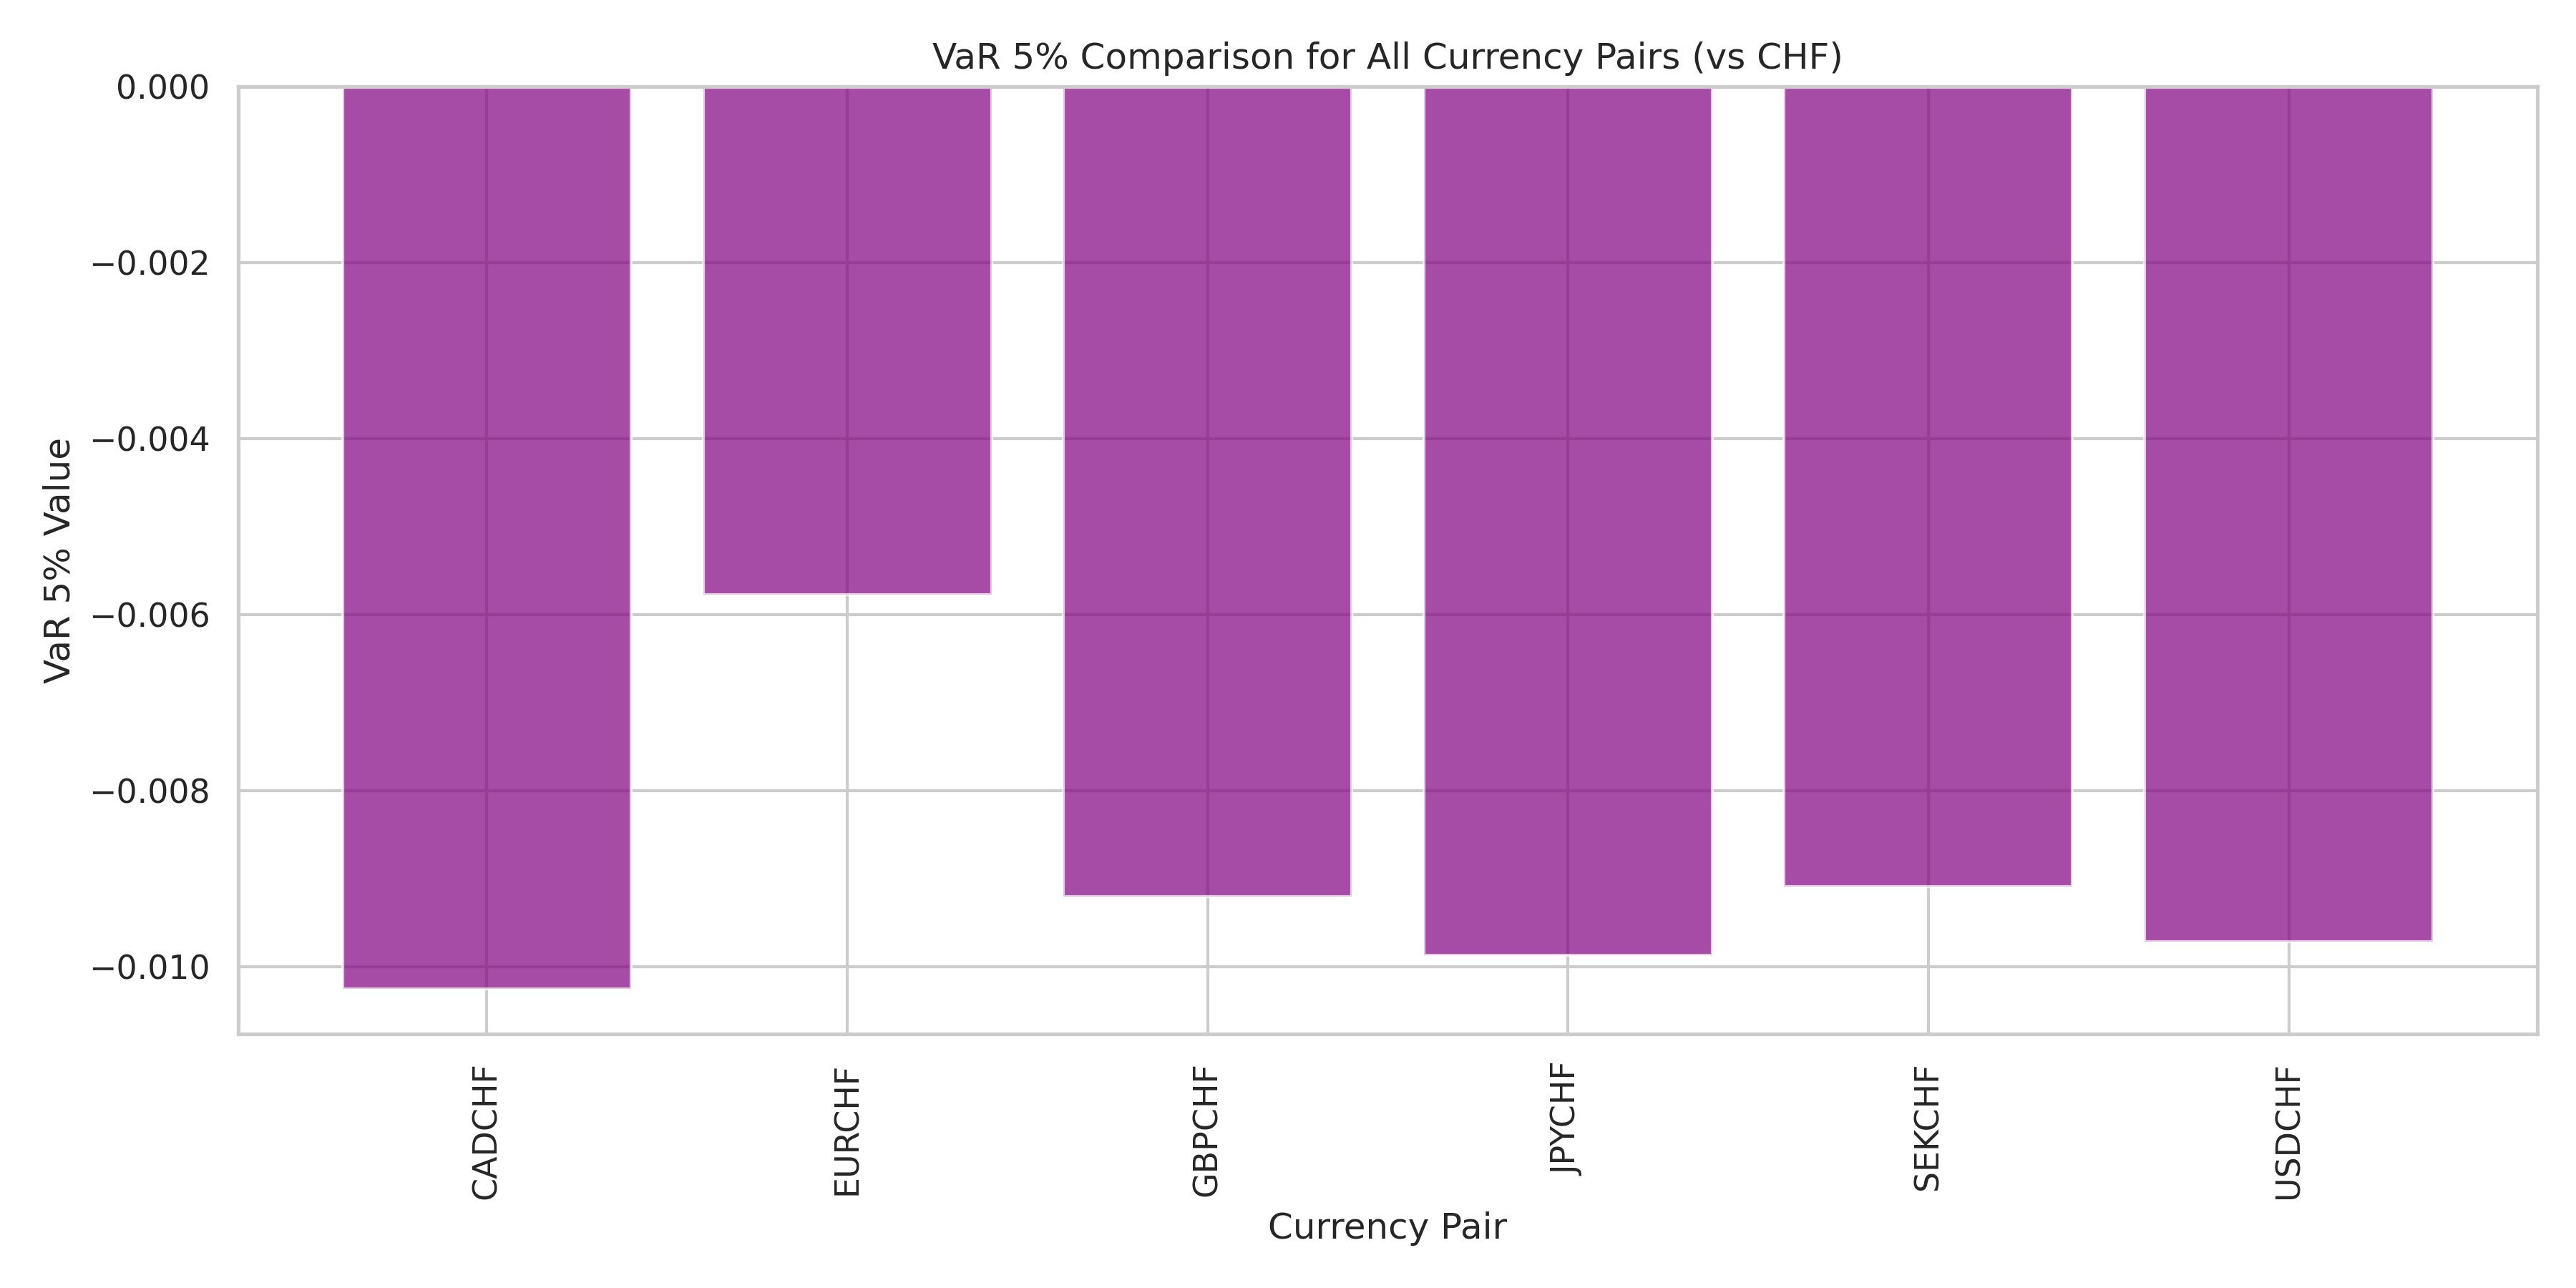
\includegraphics[width=0.5\linewidth]{reports/figures/var_5_percent_comparison_plot.png}
    \caption{5\% VaR Comparison Plot.}
    \label{fig:var_5_percent_comparison_plot}
\end{figure}
\end{frame}
% ---------------------------------------------------------------------------
\begin{frame}
\frametitle{Main Findings}
\begin{figure}
    \centering  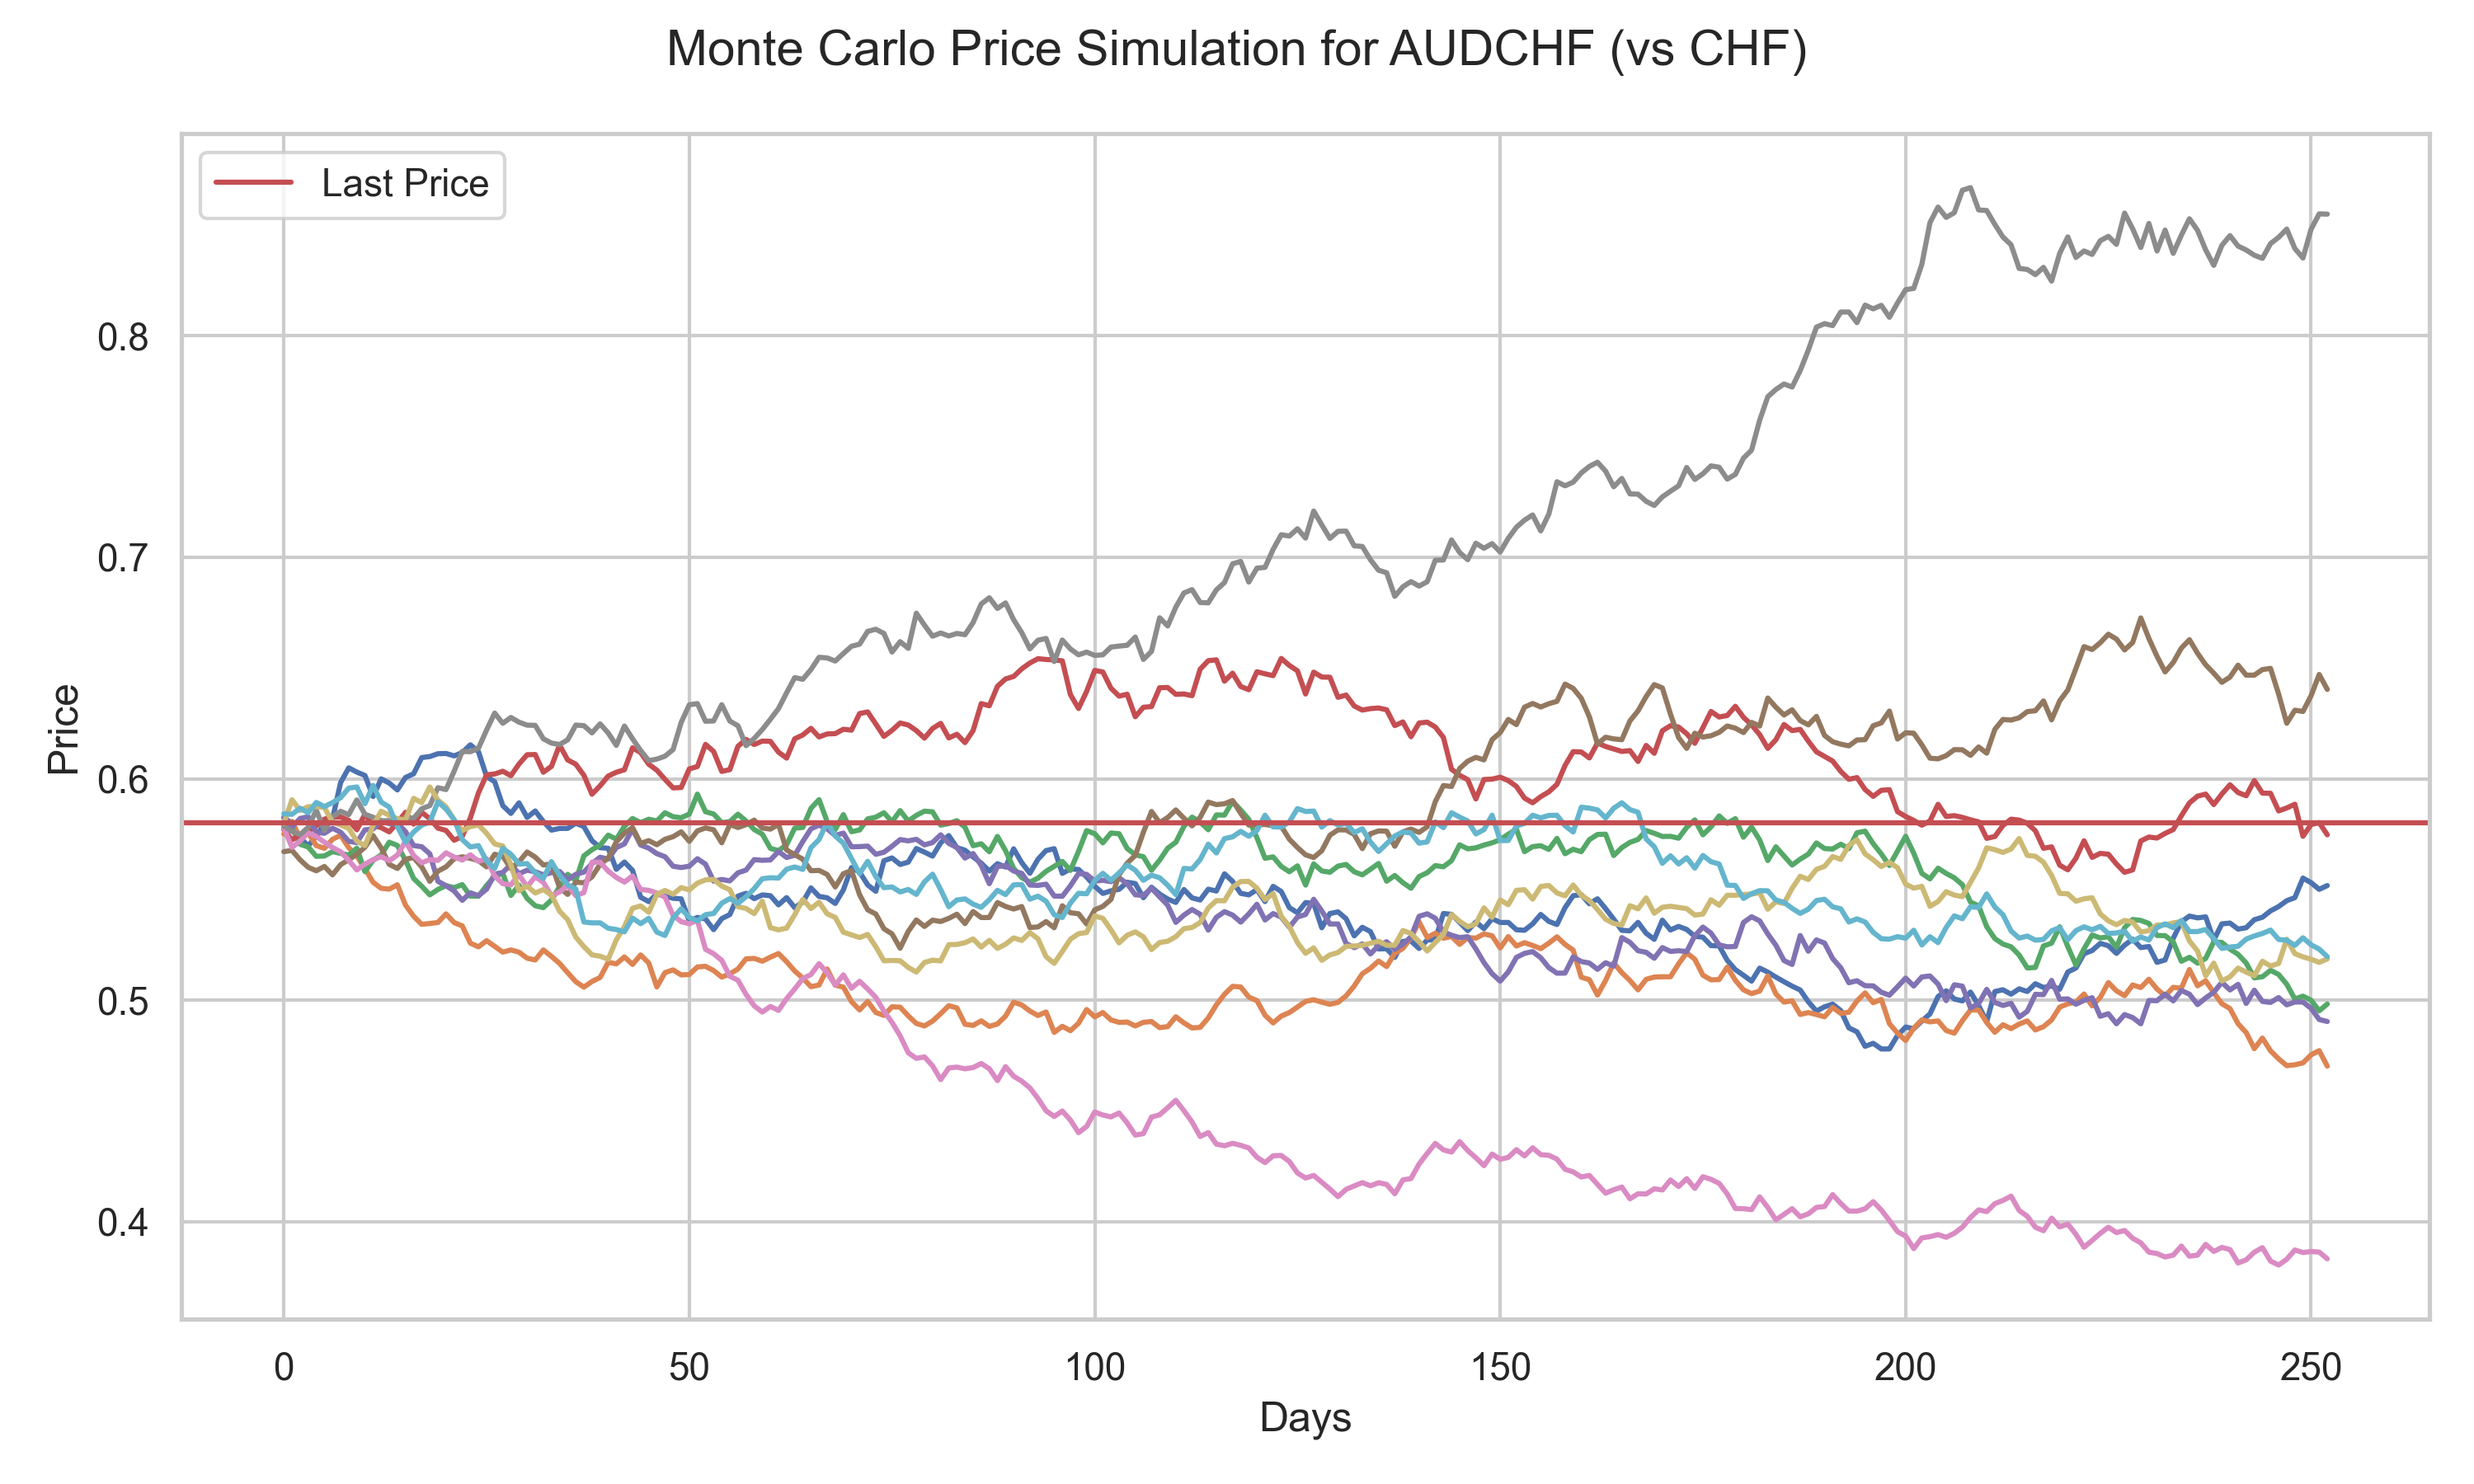
\includegraphics[width=0.48\linewidth]{reports/figures/monte_carlo_price_simulation_AUDCHF_vs_CHF.png}  \label{fig:monte_carlo_price_simulation_AUDCHF_vs_CHF}
    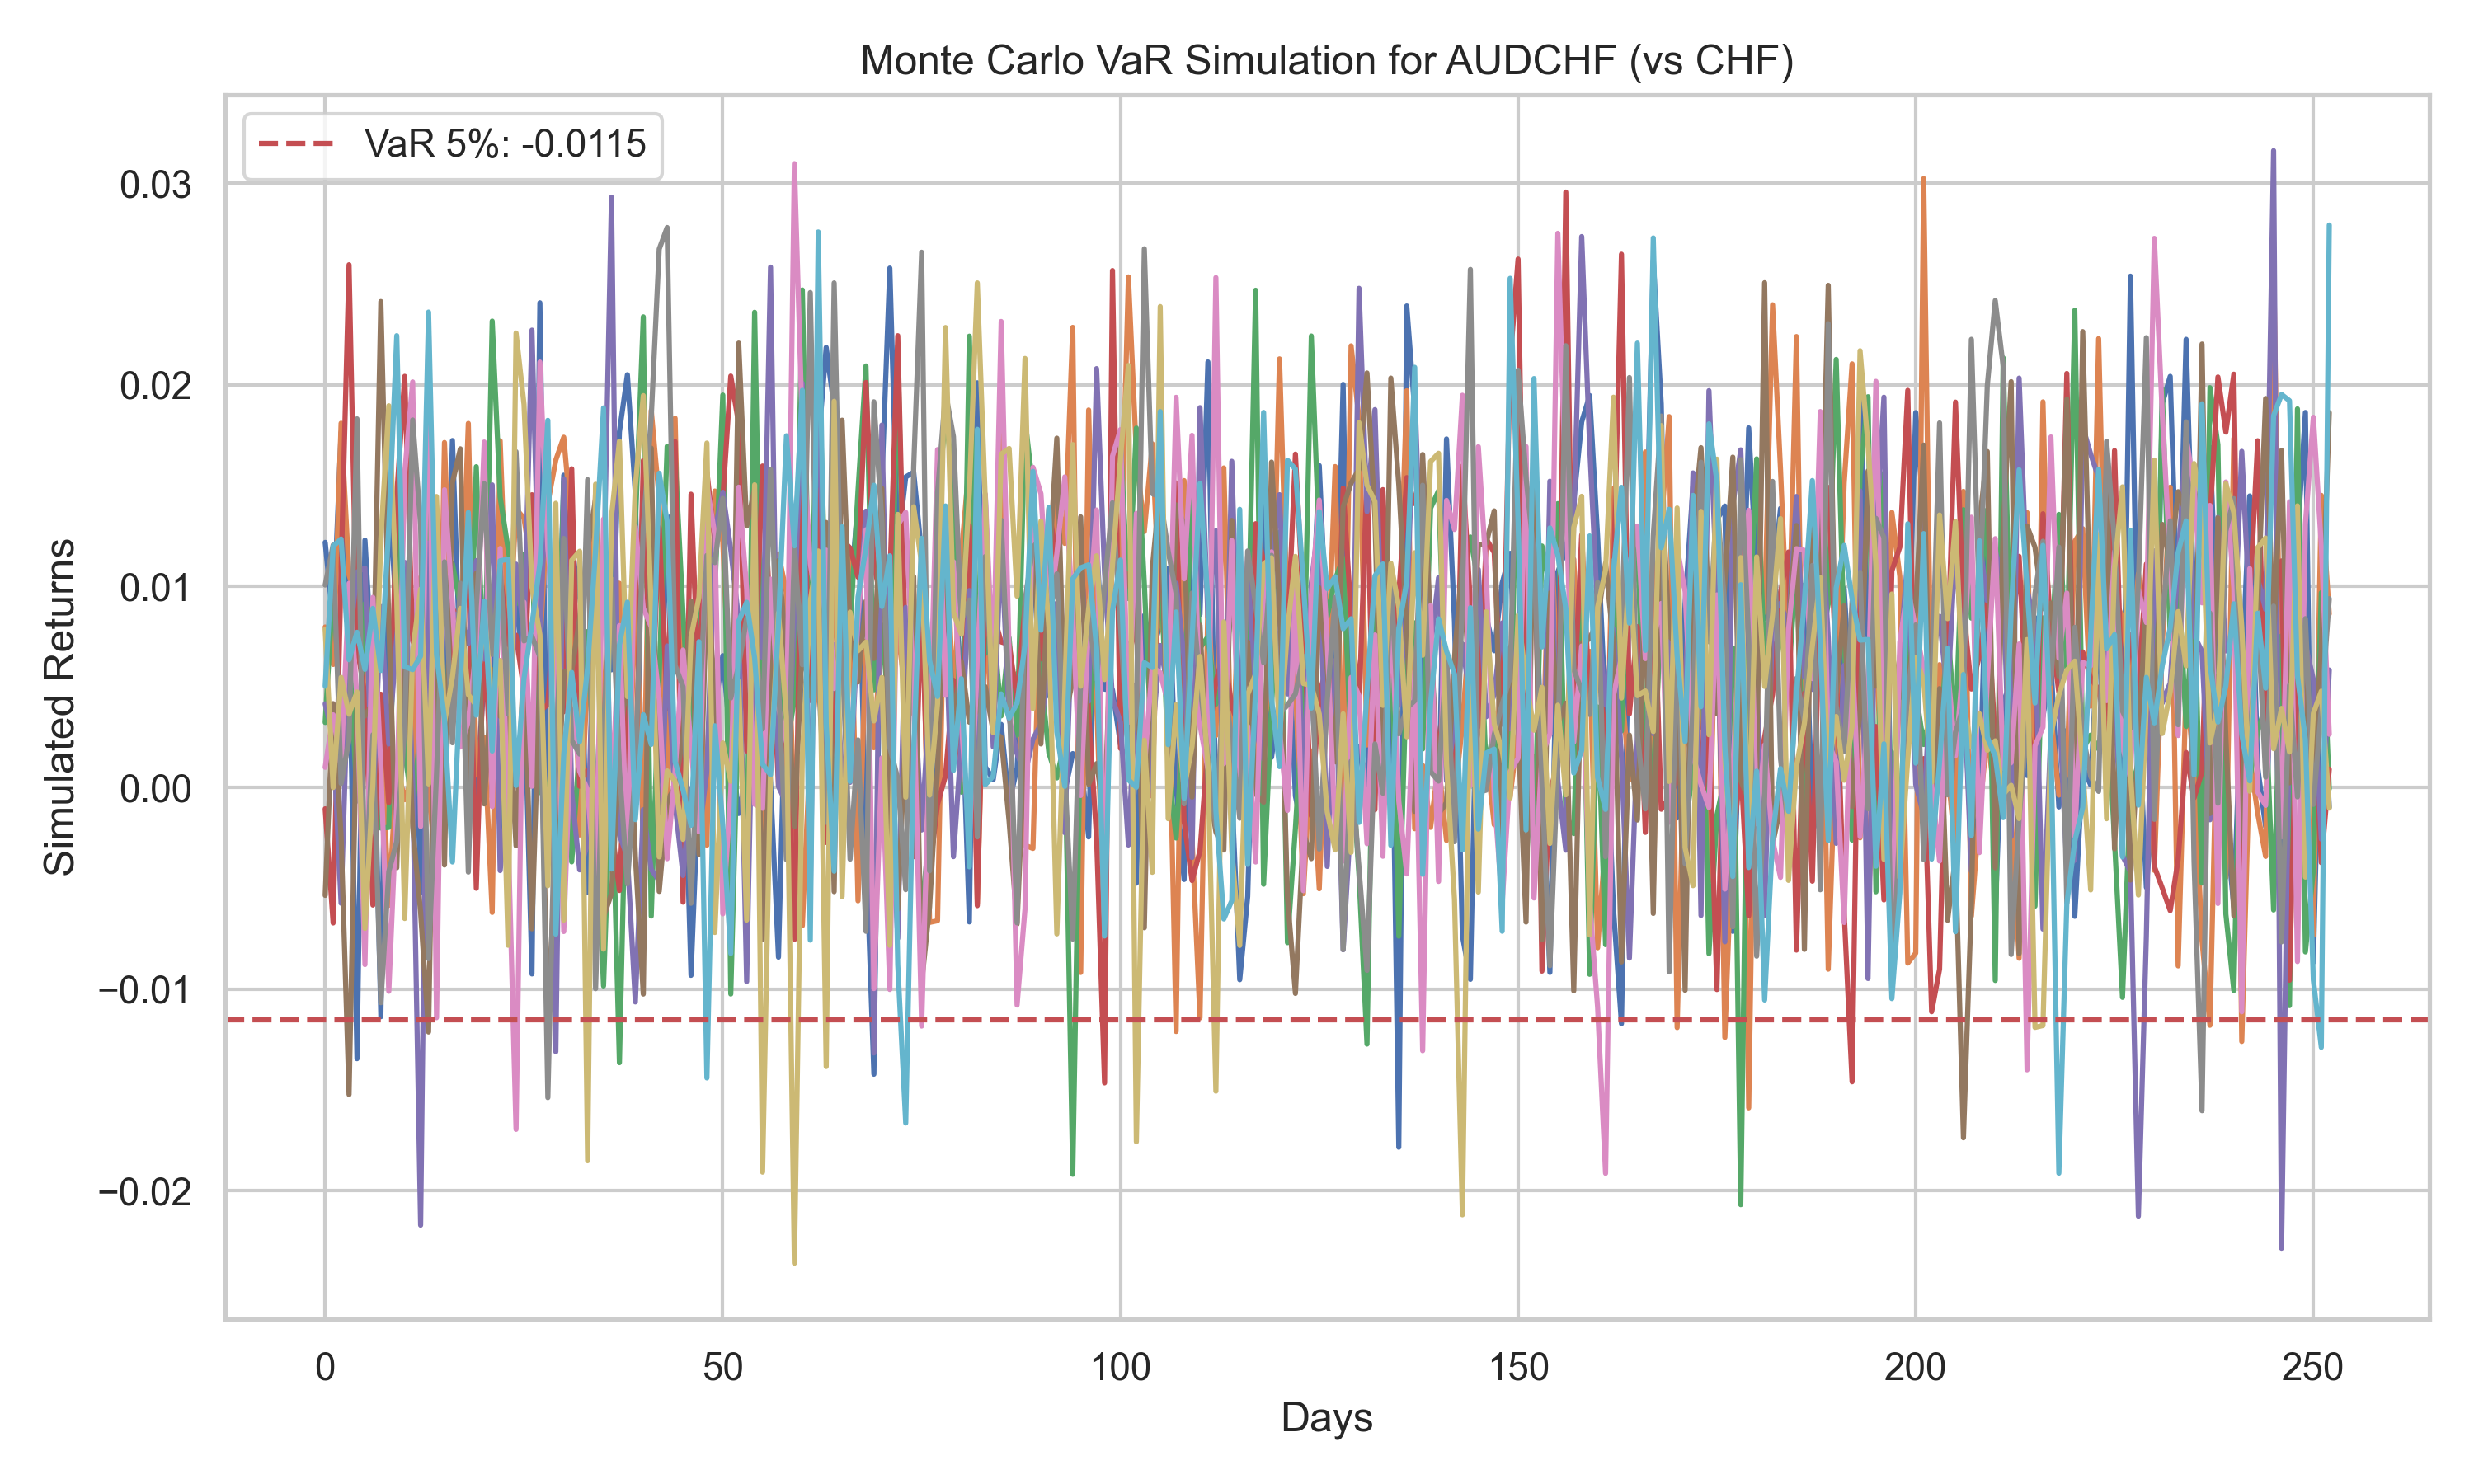
\includegraphics[width=0.48\linewidth]{reports/figures/monte_carlo_var_simulation_AUDCHF_vs_CHF.png}  \label{fig:monte_carlo_var_simulation_AUDCHF_vs_CHF}
    \caption{\footnotesize Monte Carlo price siulation (left) and VaR simulation (right) for AUD-CHF.}
\end{figure}
\begin{figure}
    \centering  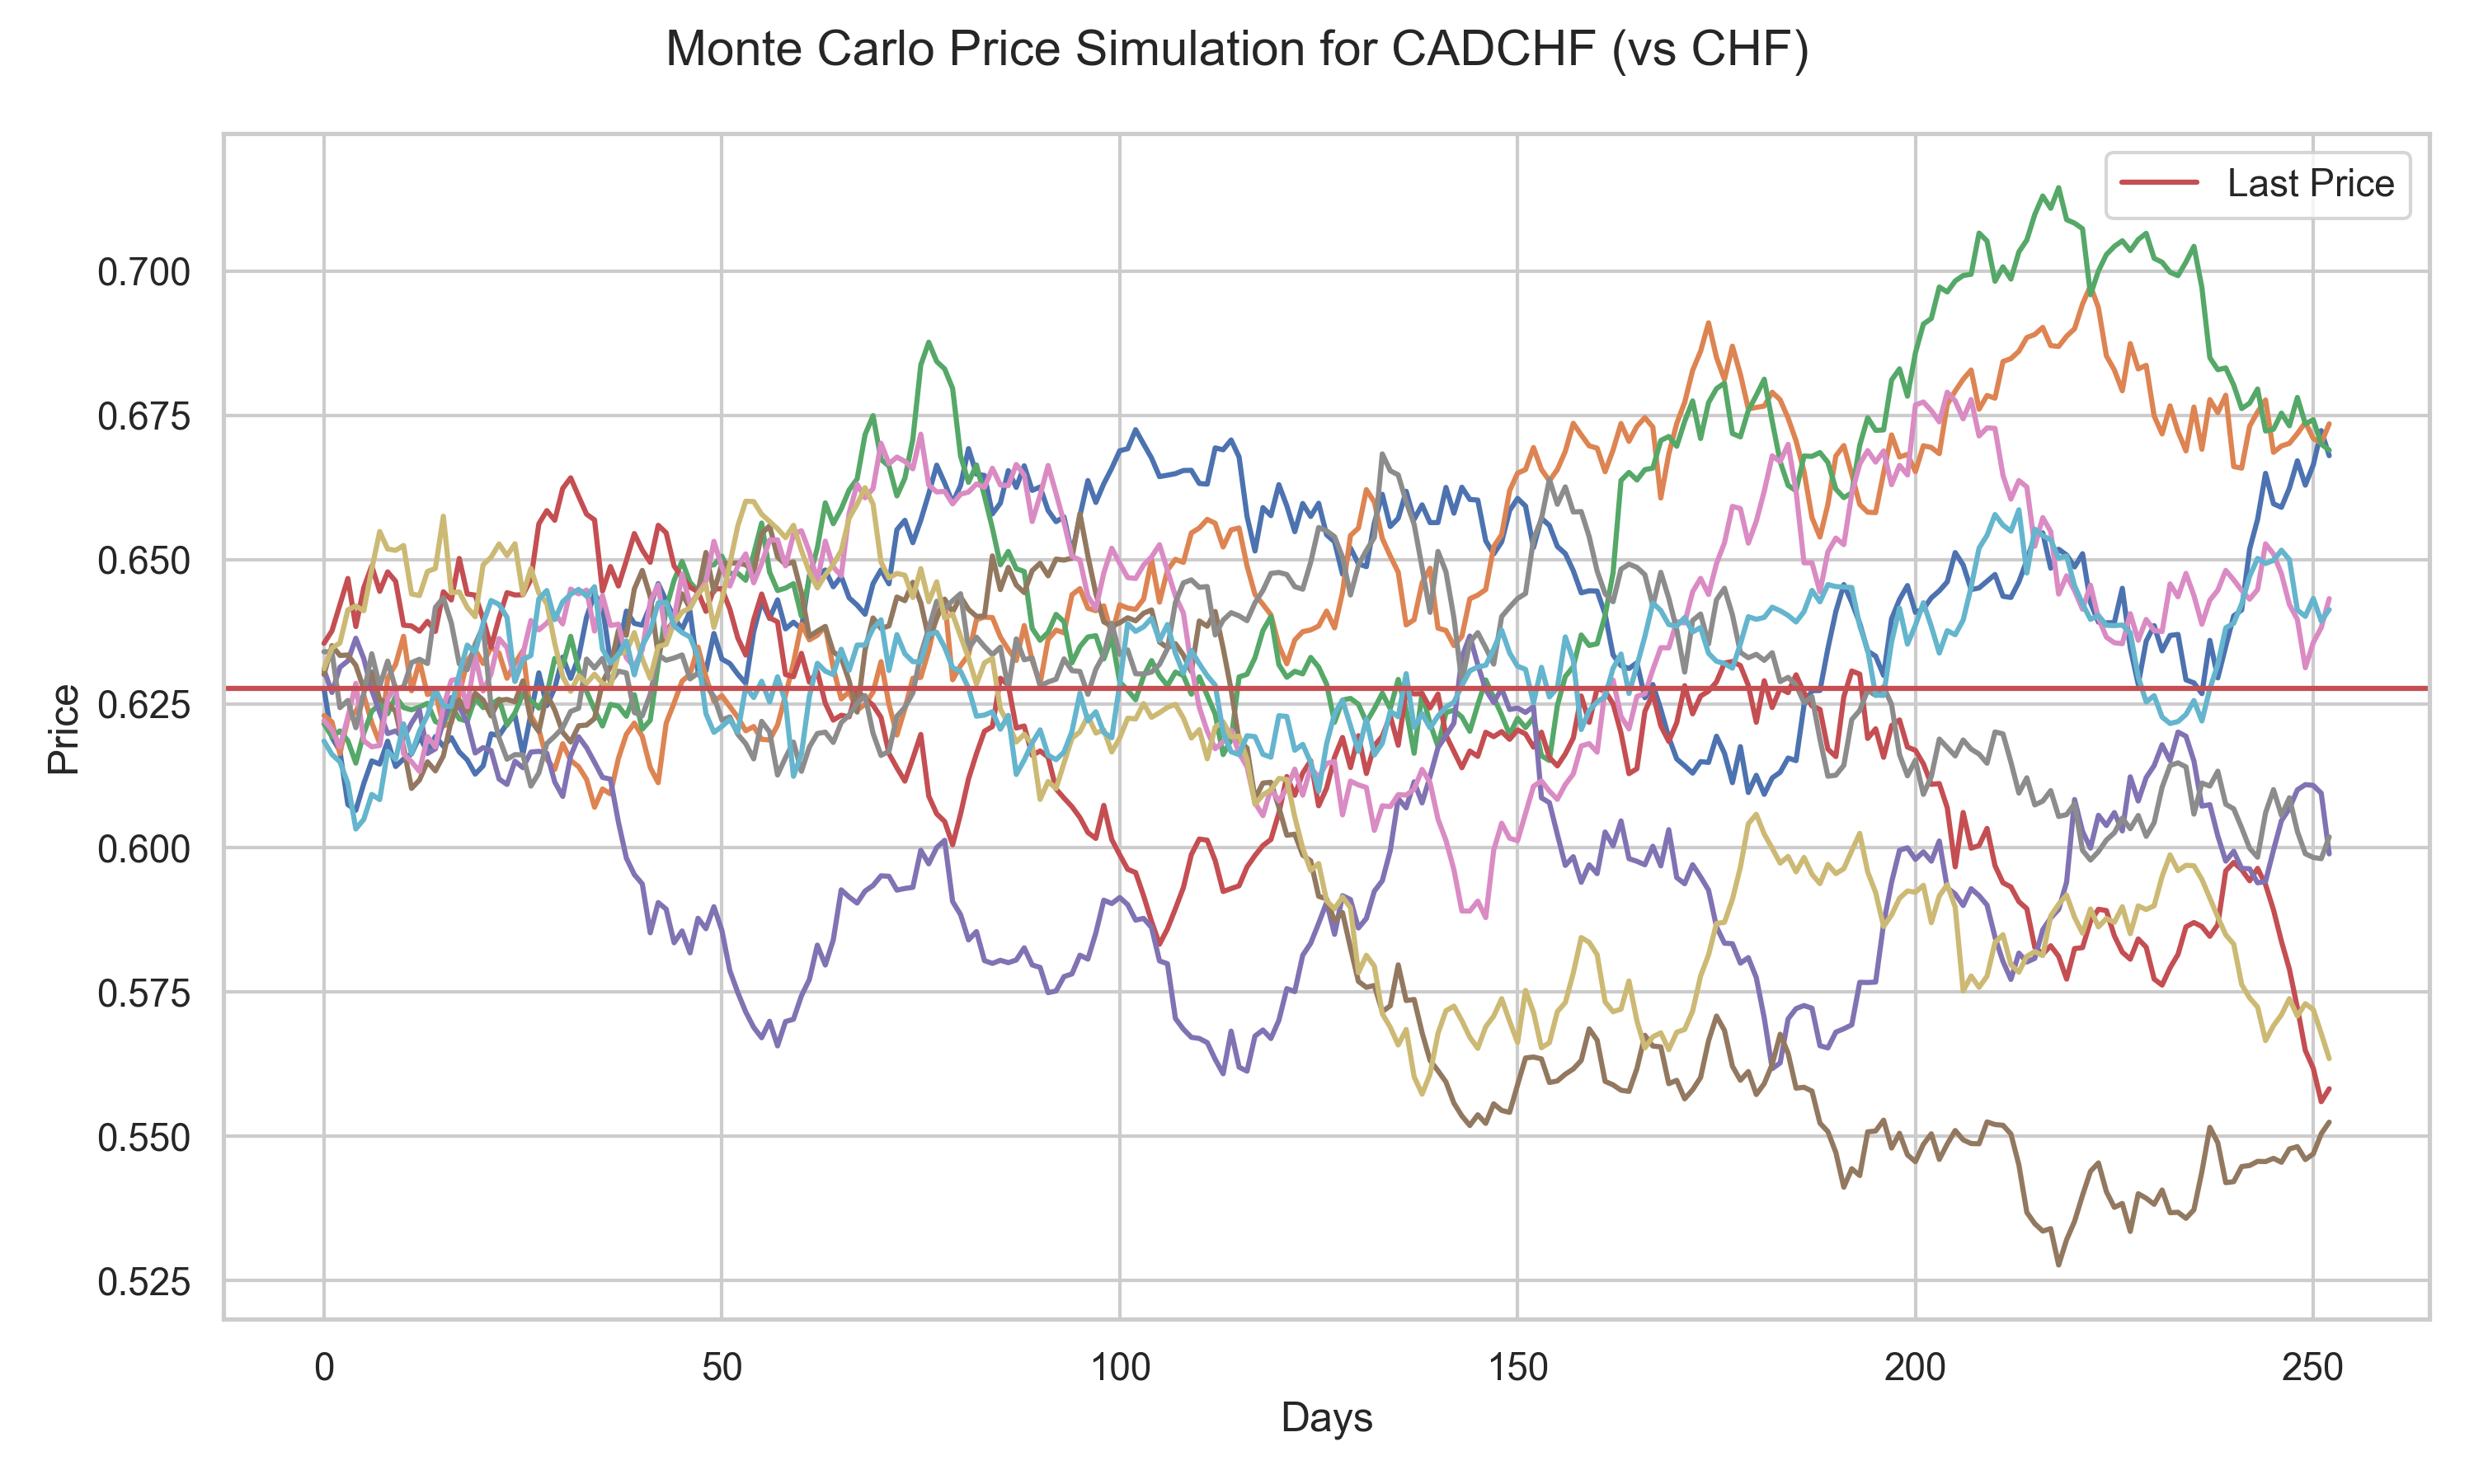
\includegraphics[width=0.48\linewidth]{reports/figures/monte_carlo_price_simulation_CADCHF_vs_CHF.png} \label{fig:monte_carlo_price_simulation_CADCHF_vs_CHF}
    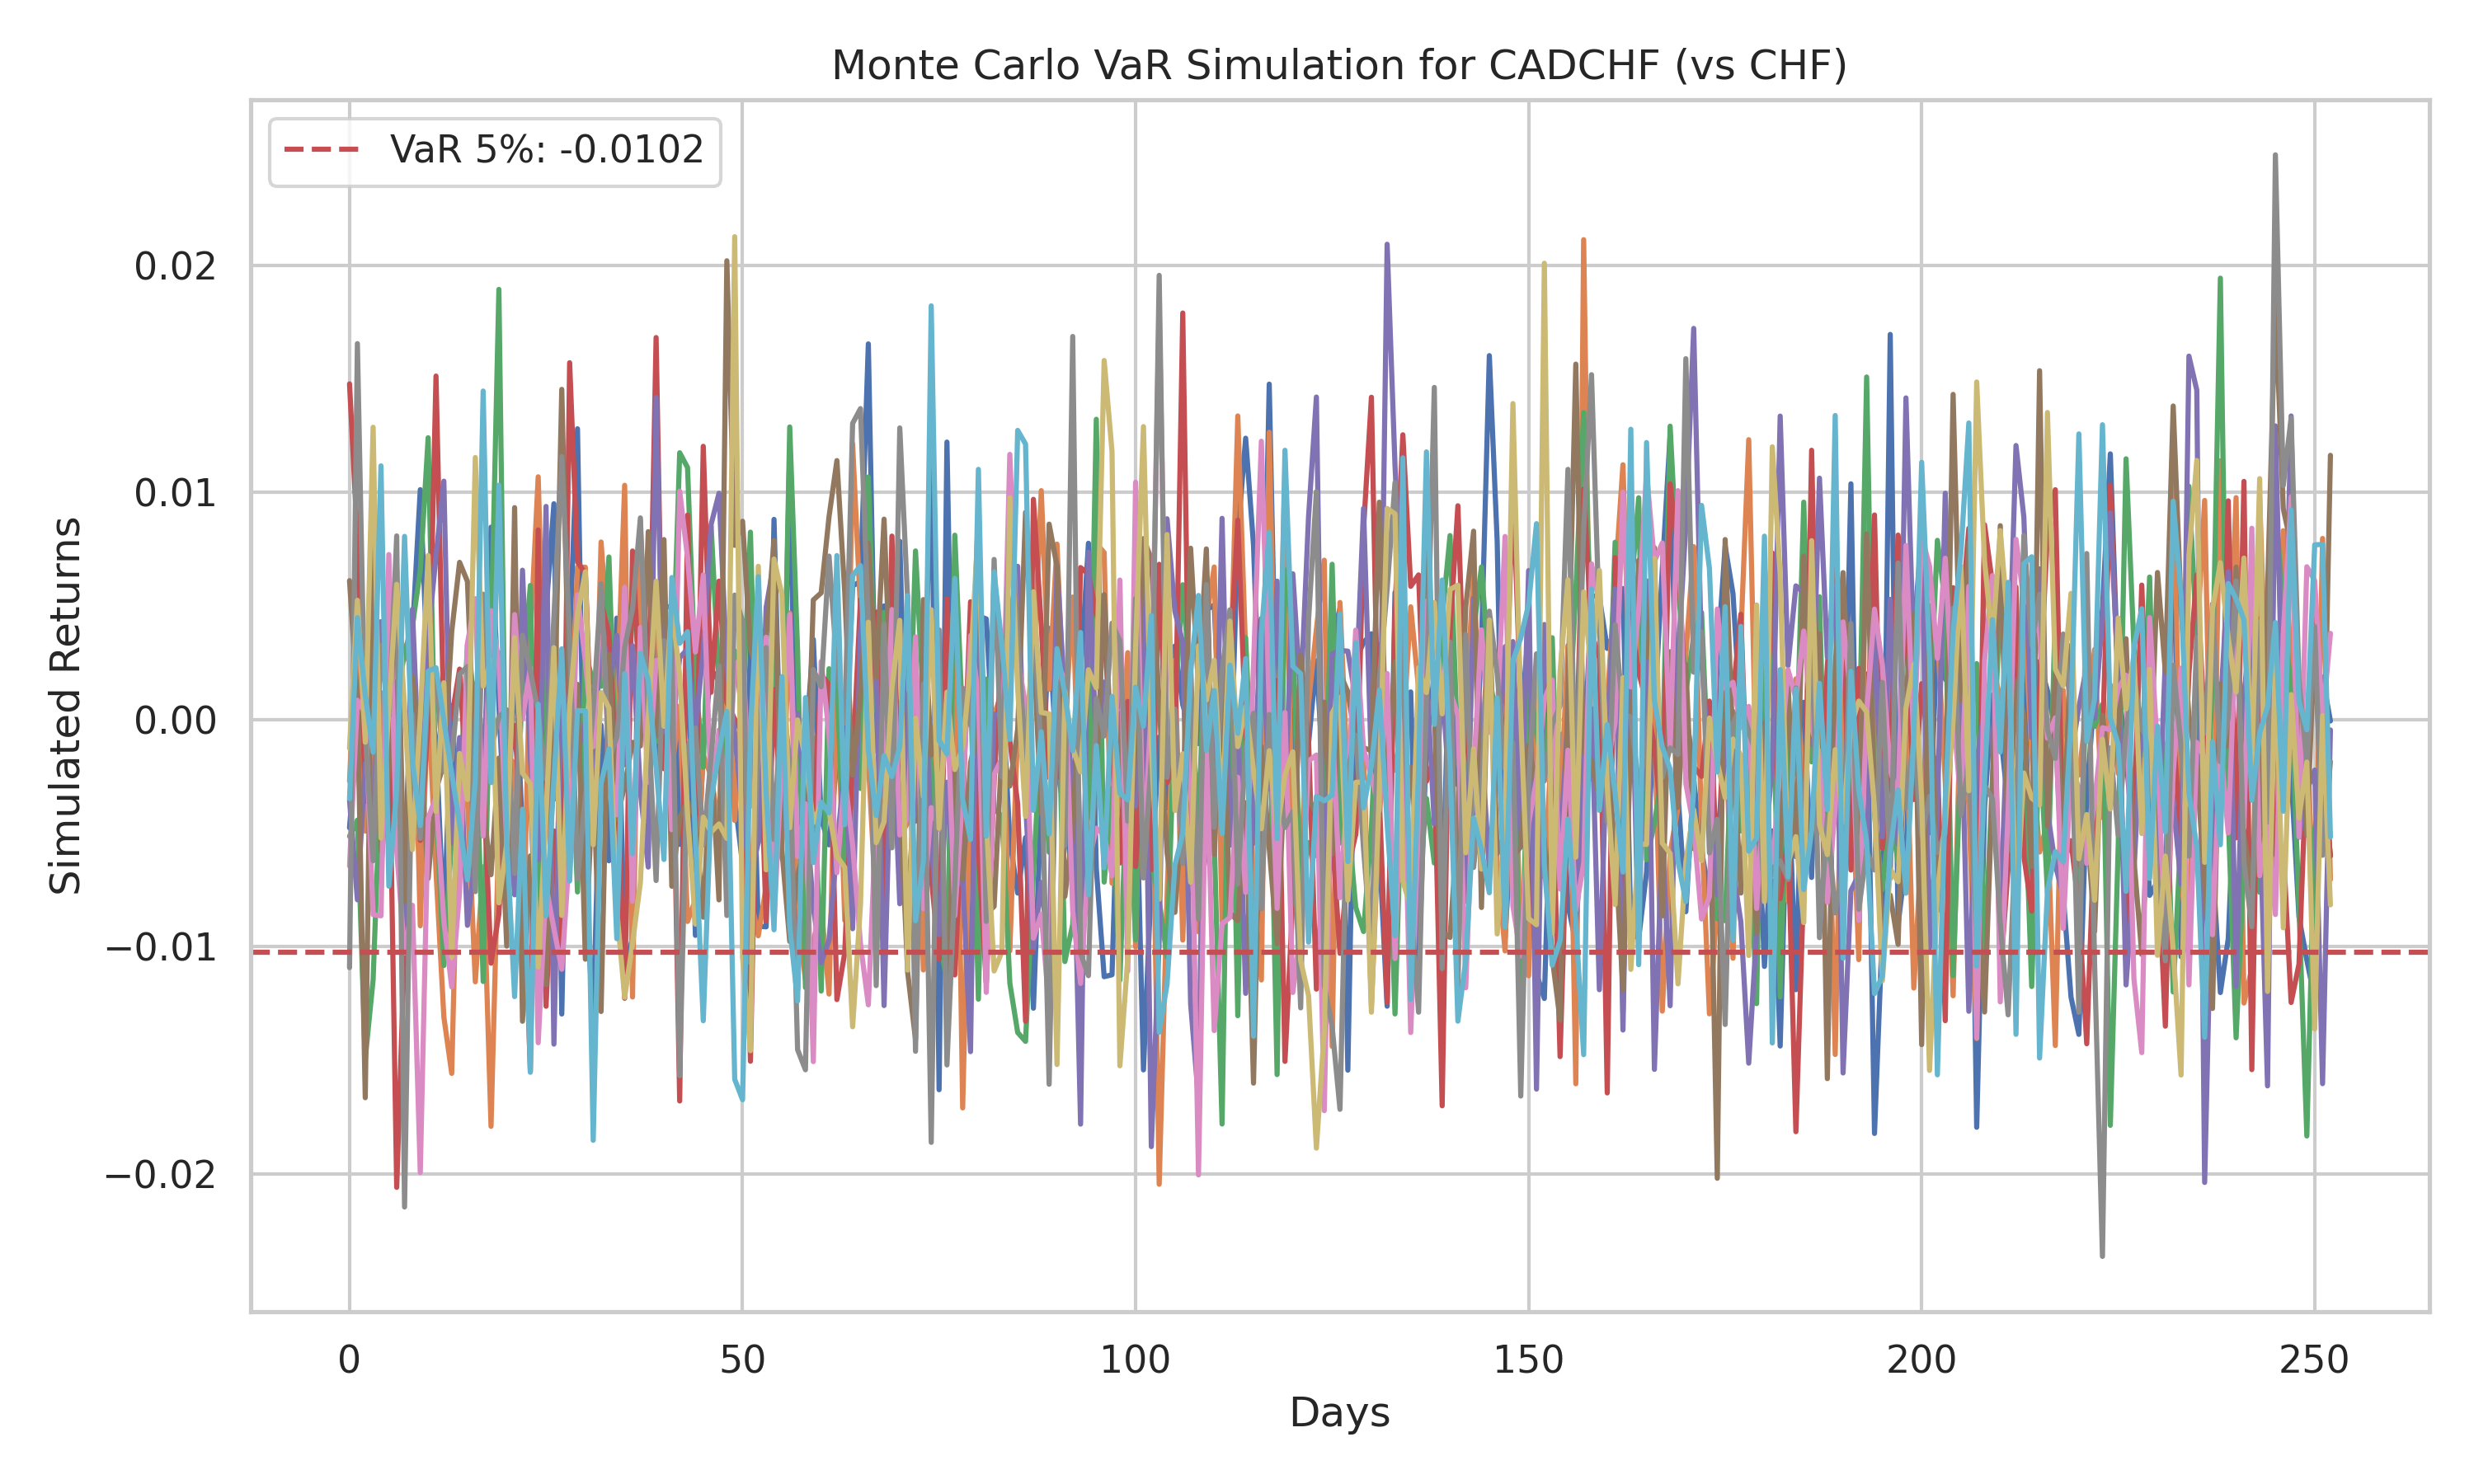
\includegraphics[width=0.48\linewidth]{reports/figures/monte_carlo_var_simulation_CADCHF_vs_CHF.png} \label{fig:monte_carlo_var_simulation_CADCHF_vs_CHF}
    \caption{\footnotesize Monte Carlo price siulation (left) and VaR simulation (right) for CAD-CHF.}
\end{figure}
\end{frame}
% ---------------------------------------------------------------------------
\begin{frame}
\frametitle{Main Findings}
\begin{figure}
    \centering  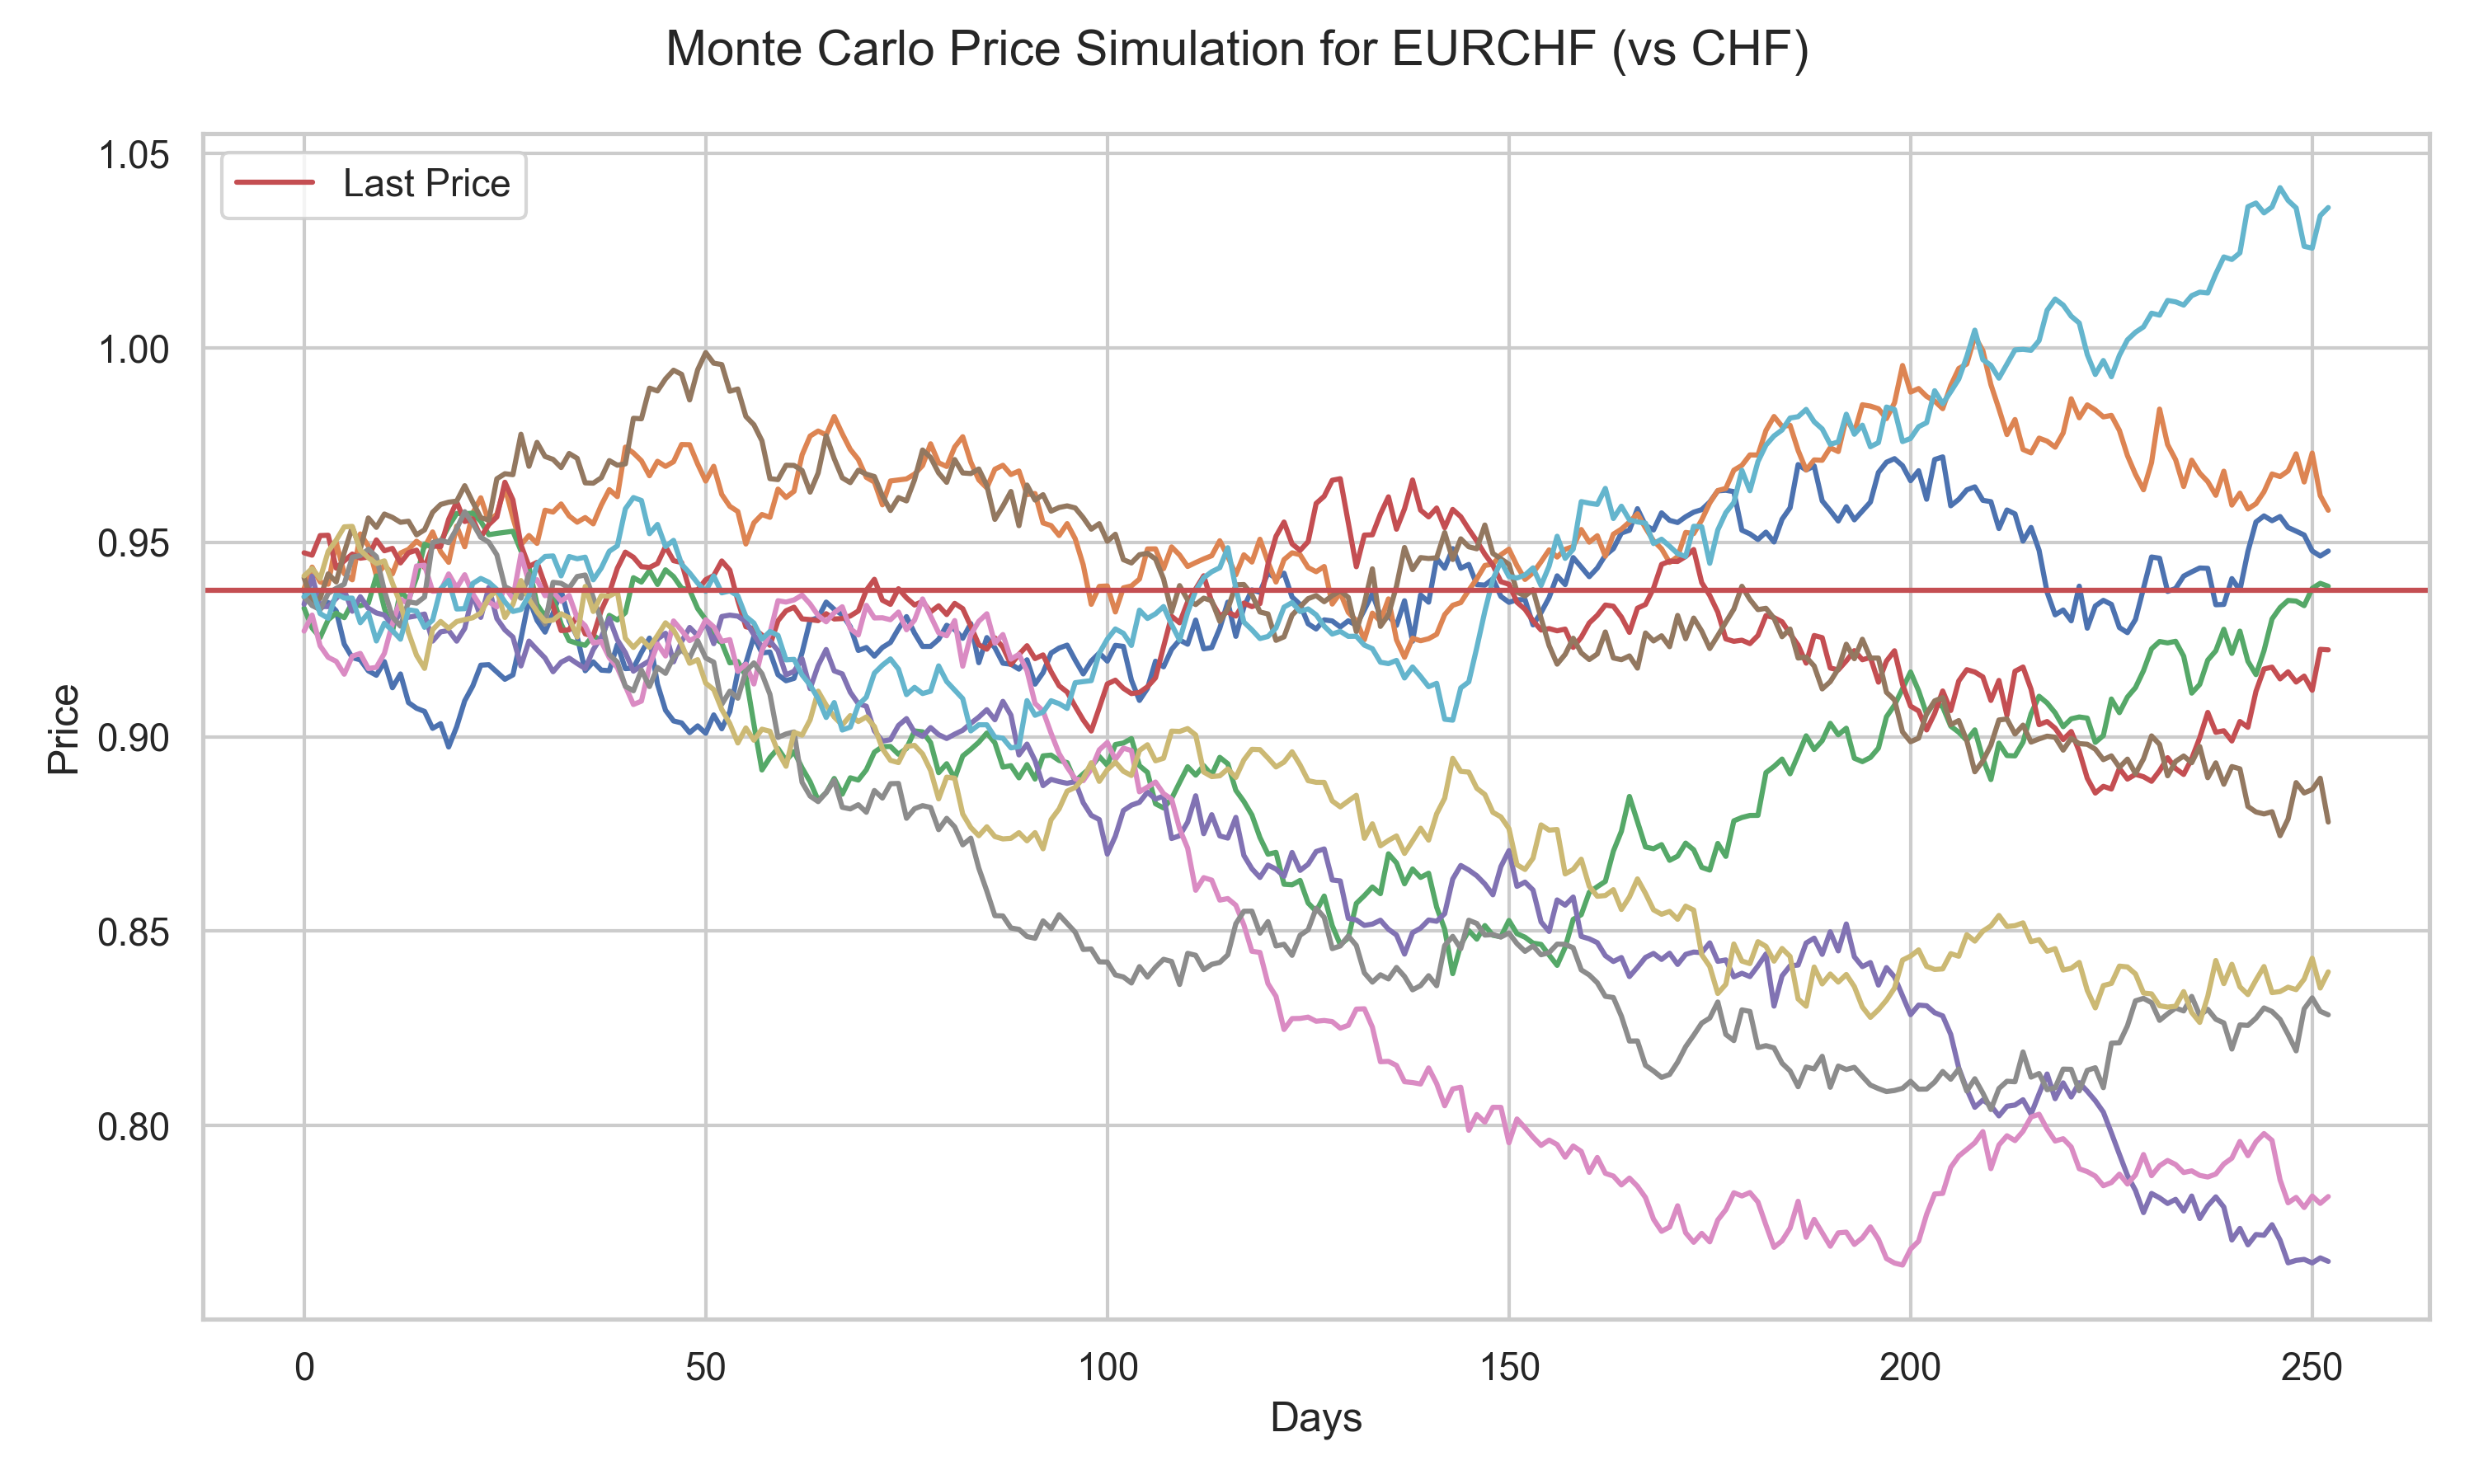
\includegraphics[width=0.48\linewidth]{reports/figures/monte_carlo_price_simulation_EURCHF_vs_CHF.png}  \label{fig:monte_carlo_price_simulation_EURCHF_vs_CHF}
    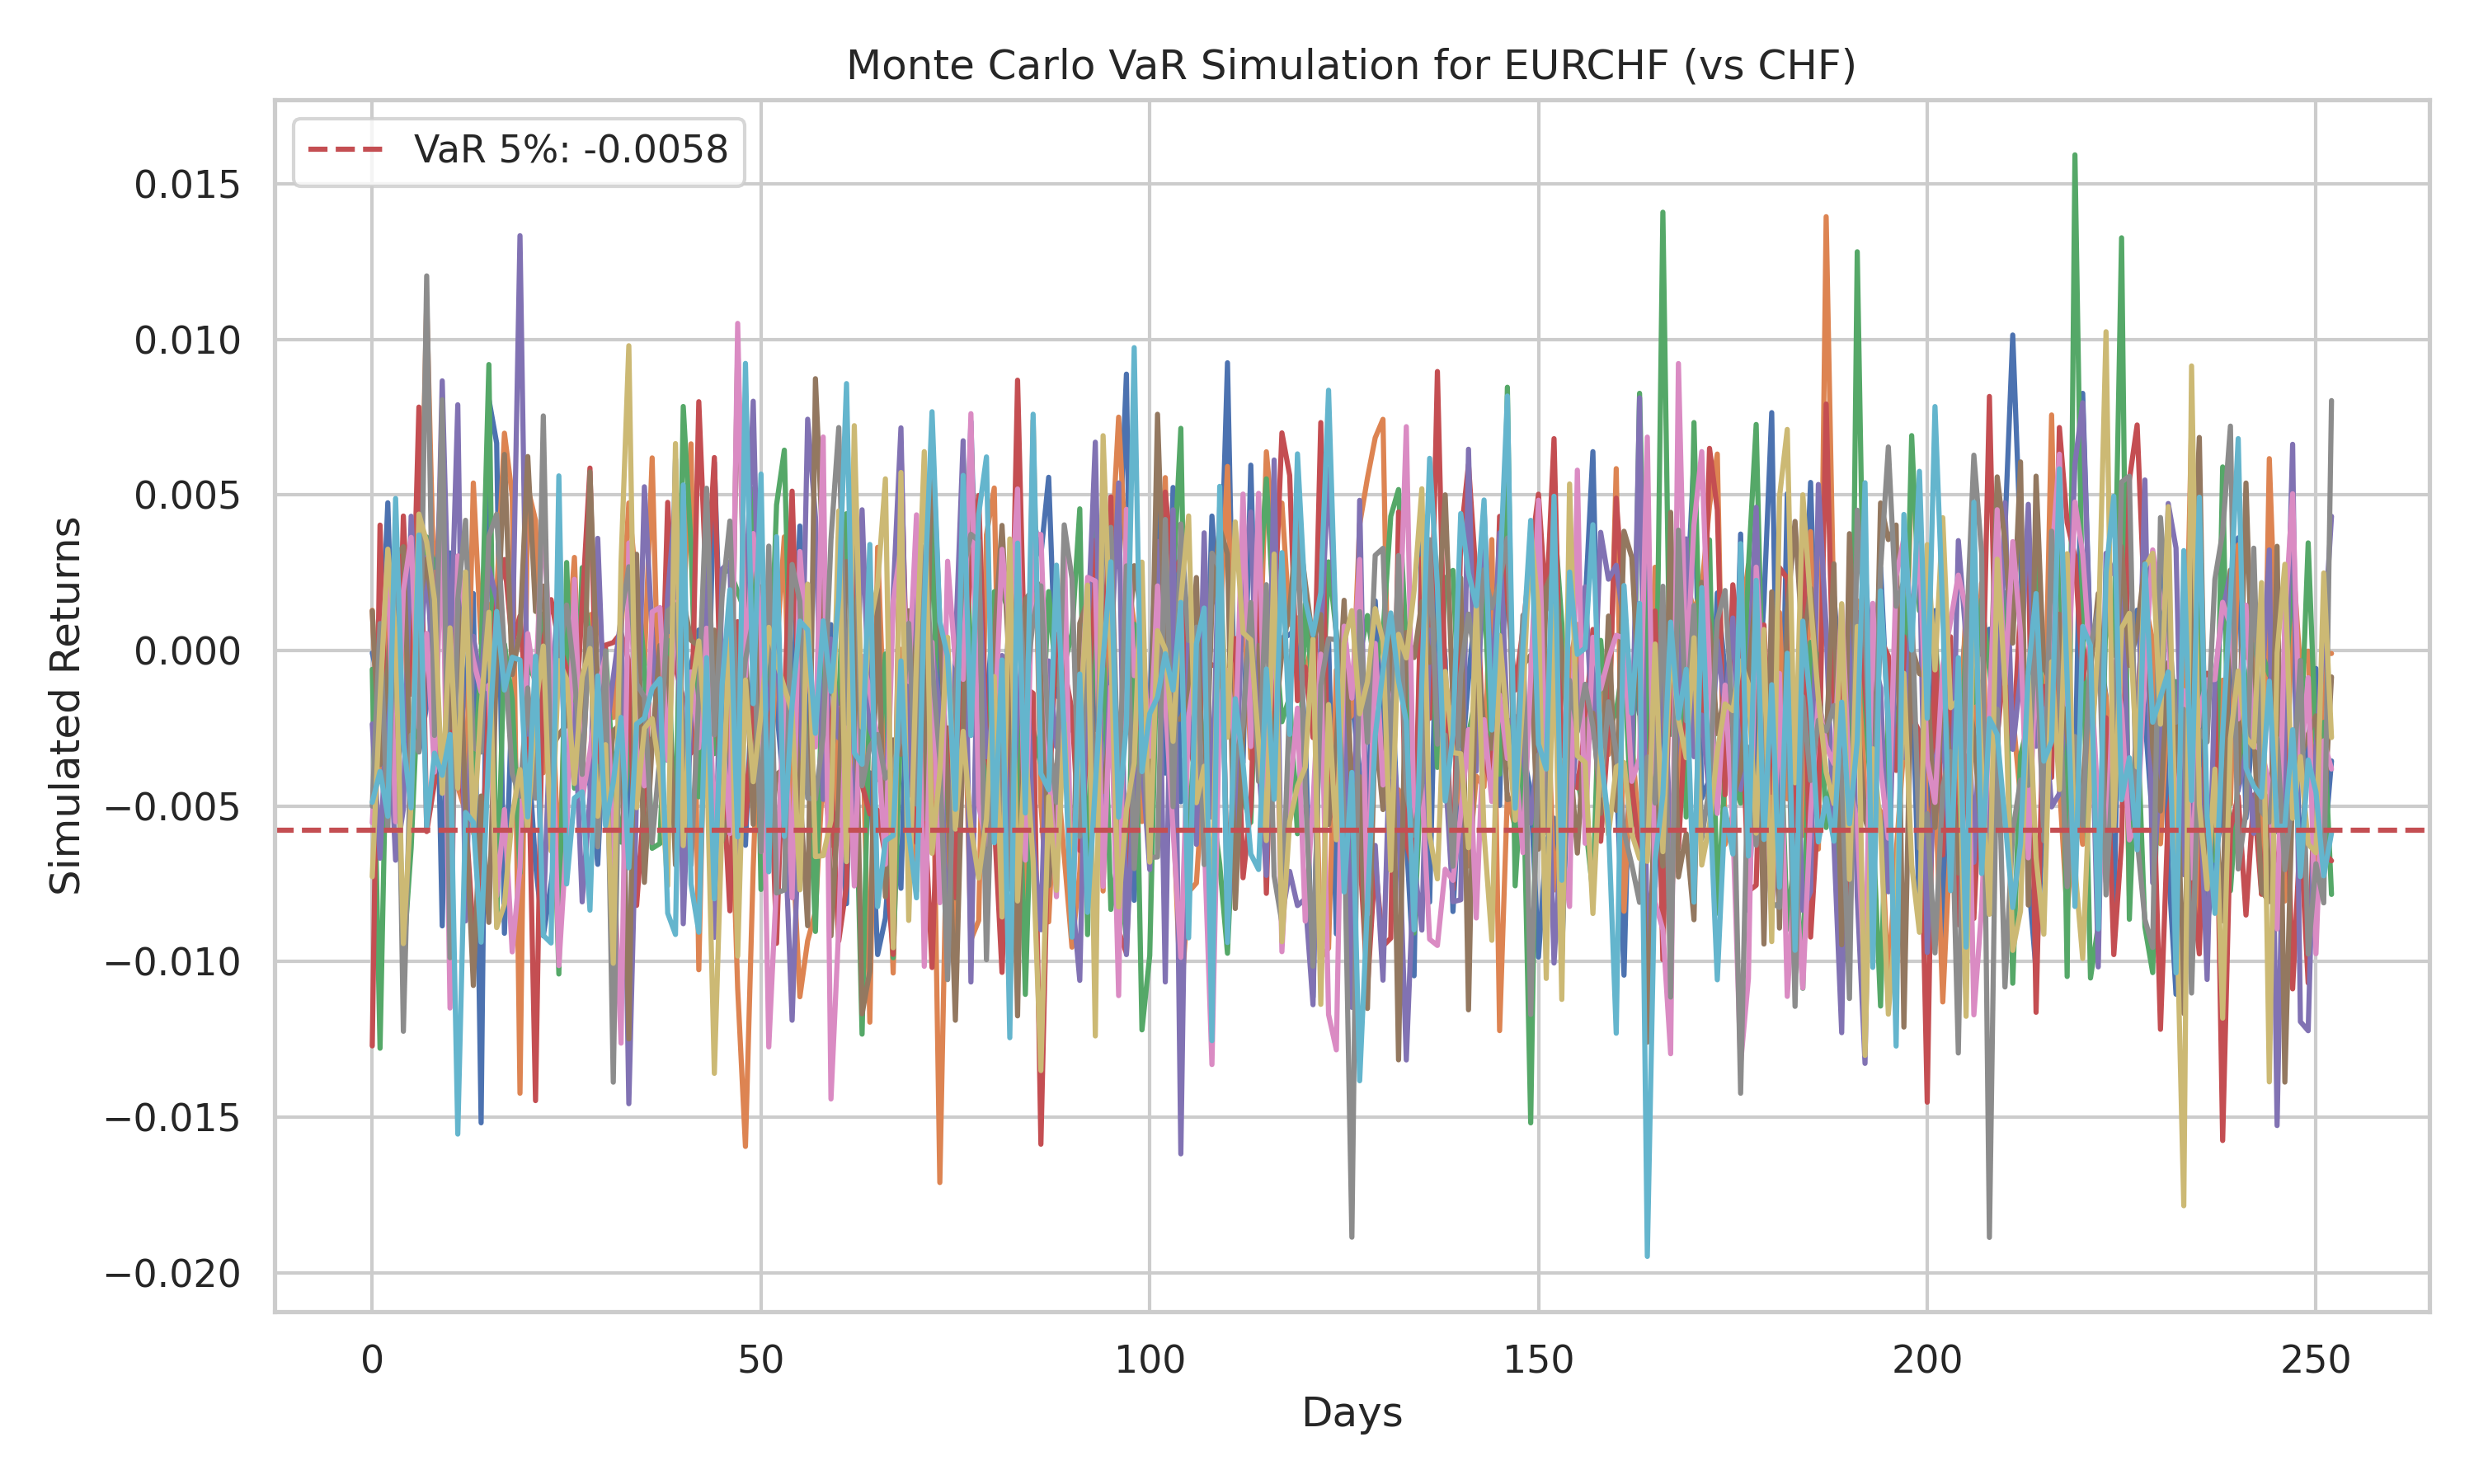
\includegraphics[width=0.48\linewidth]{reports/figures/monte_carlo_var_simulation_EURCHF_vs_CHF.png}  \label{fig:monte_carlo_var_simulation_EURCHF_vs_CHF}
    \caption{\footnotesize Monte Carlo price siulation (left) and VaR simulation (right) for EUR-CHF.}
\end{figure}
\begin{figure}
    \centering   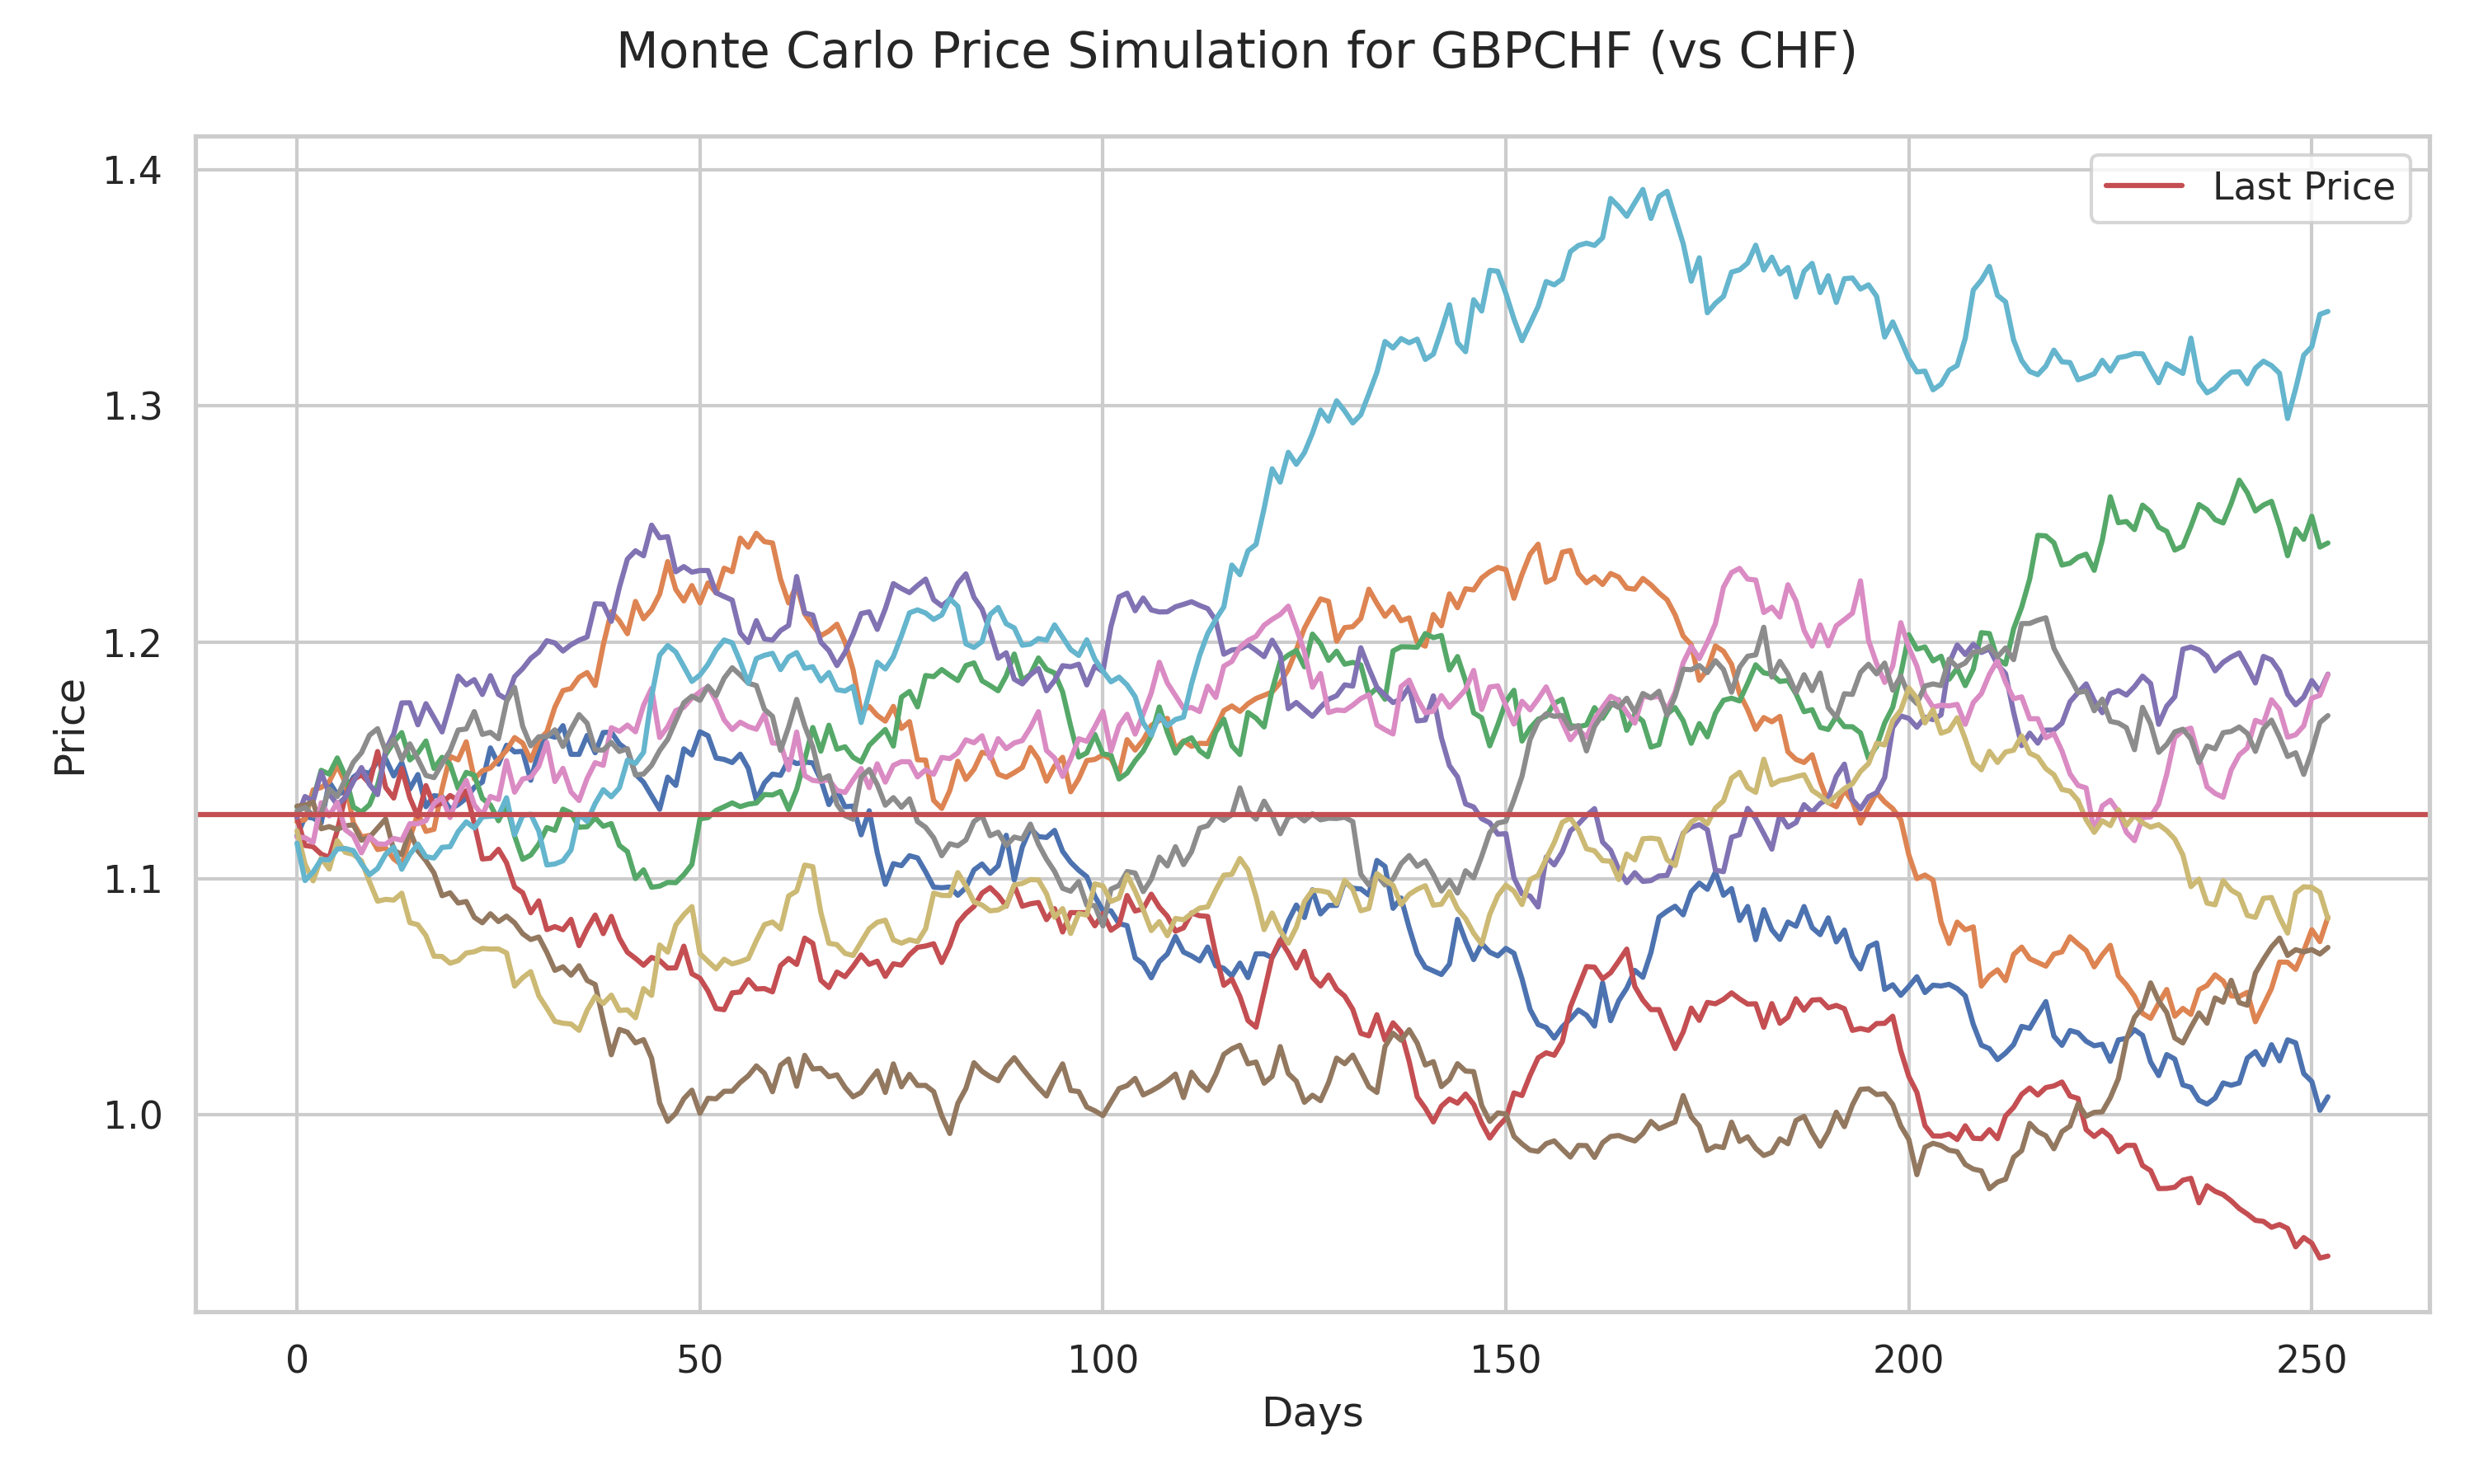
\includegraphics[width=0.48\linewidth]{reports/figures/monte_carlo_price_simulation_GBPCHF_vs_CHF.png} \label{fig:monte_carlo_price_simulation_GBPCHF_vs_CHF}
    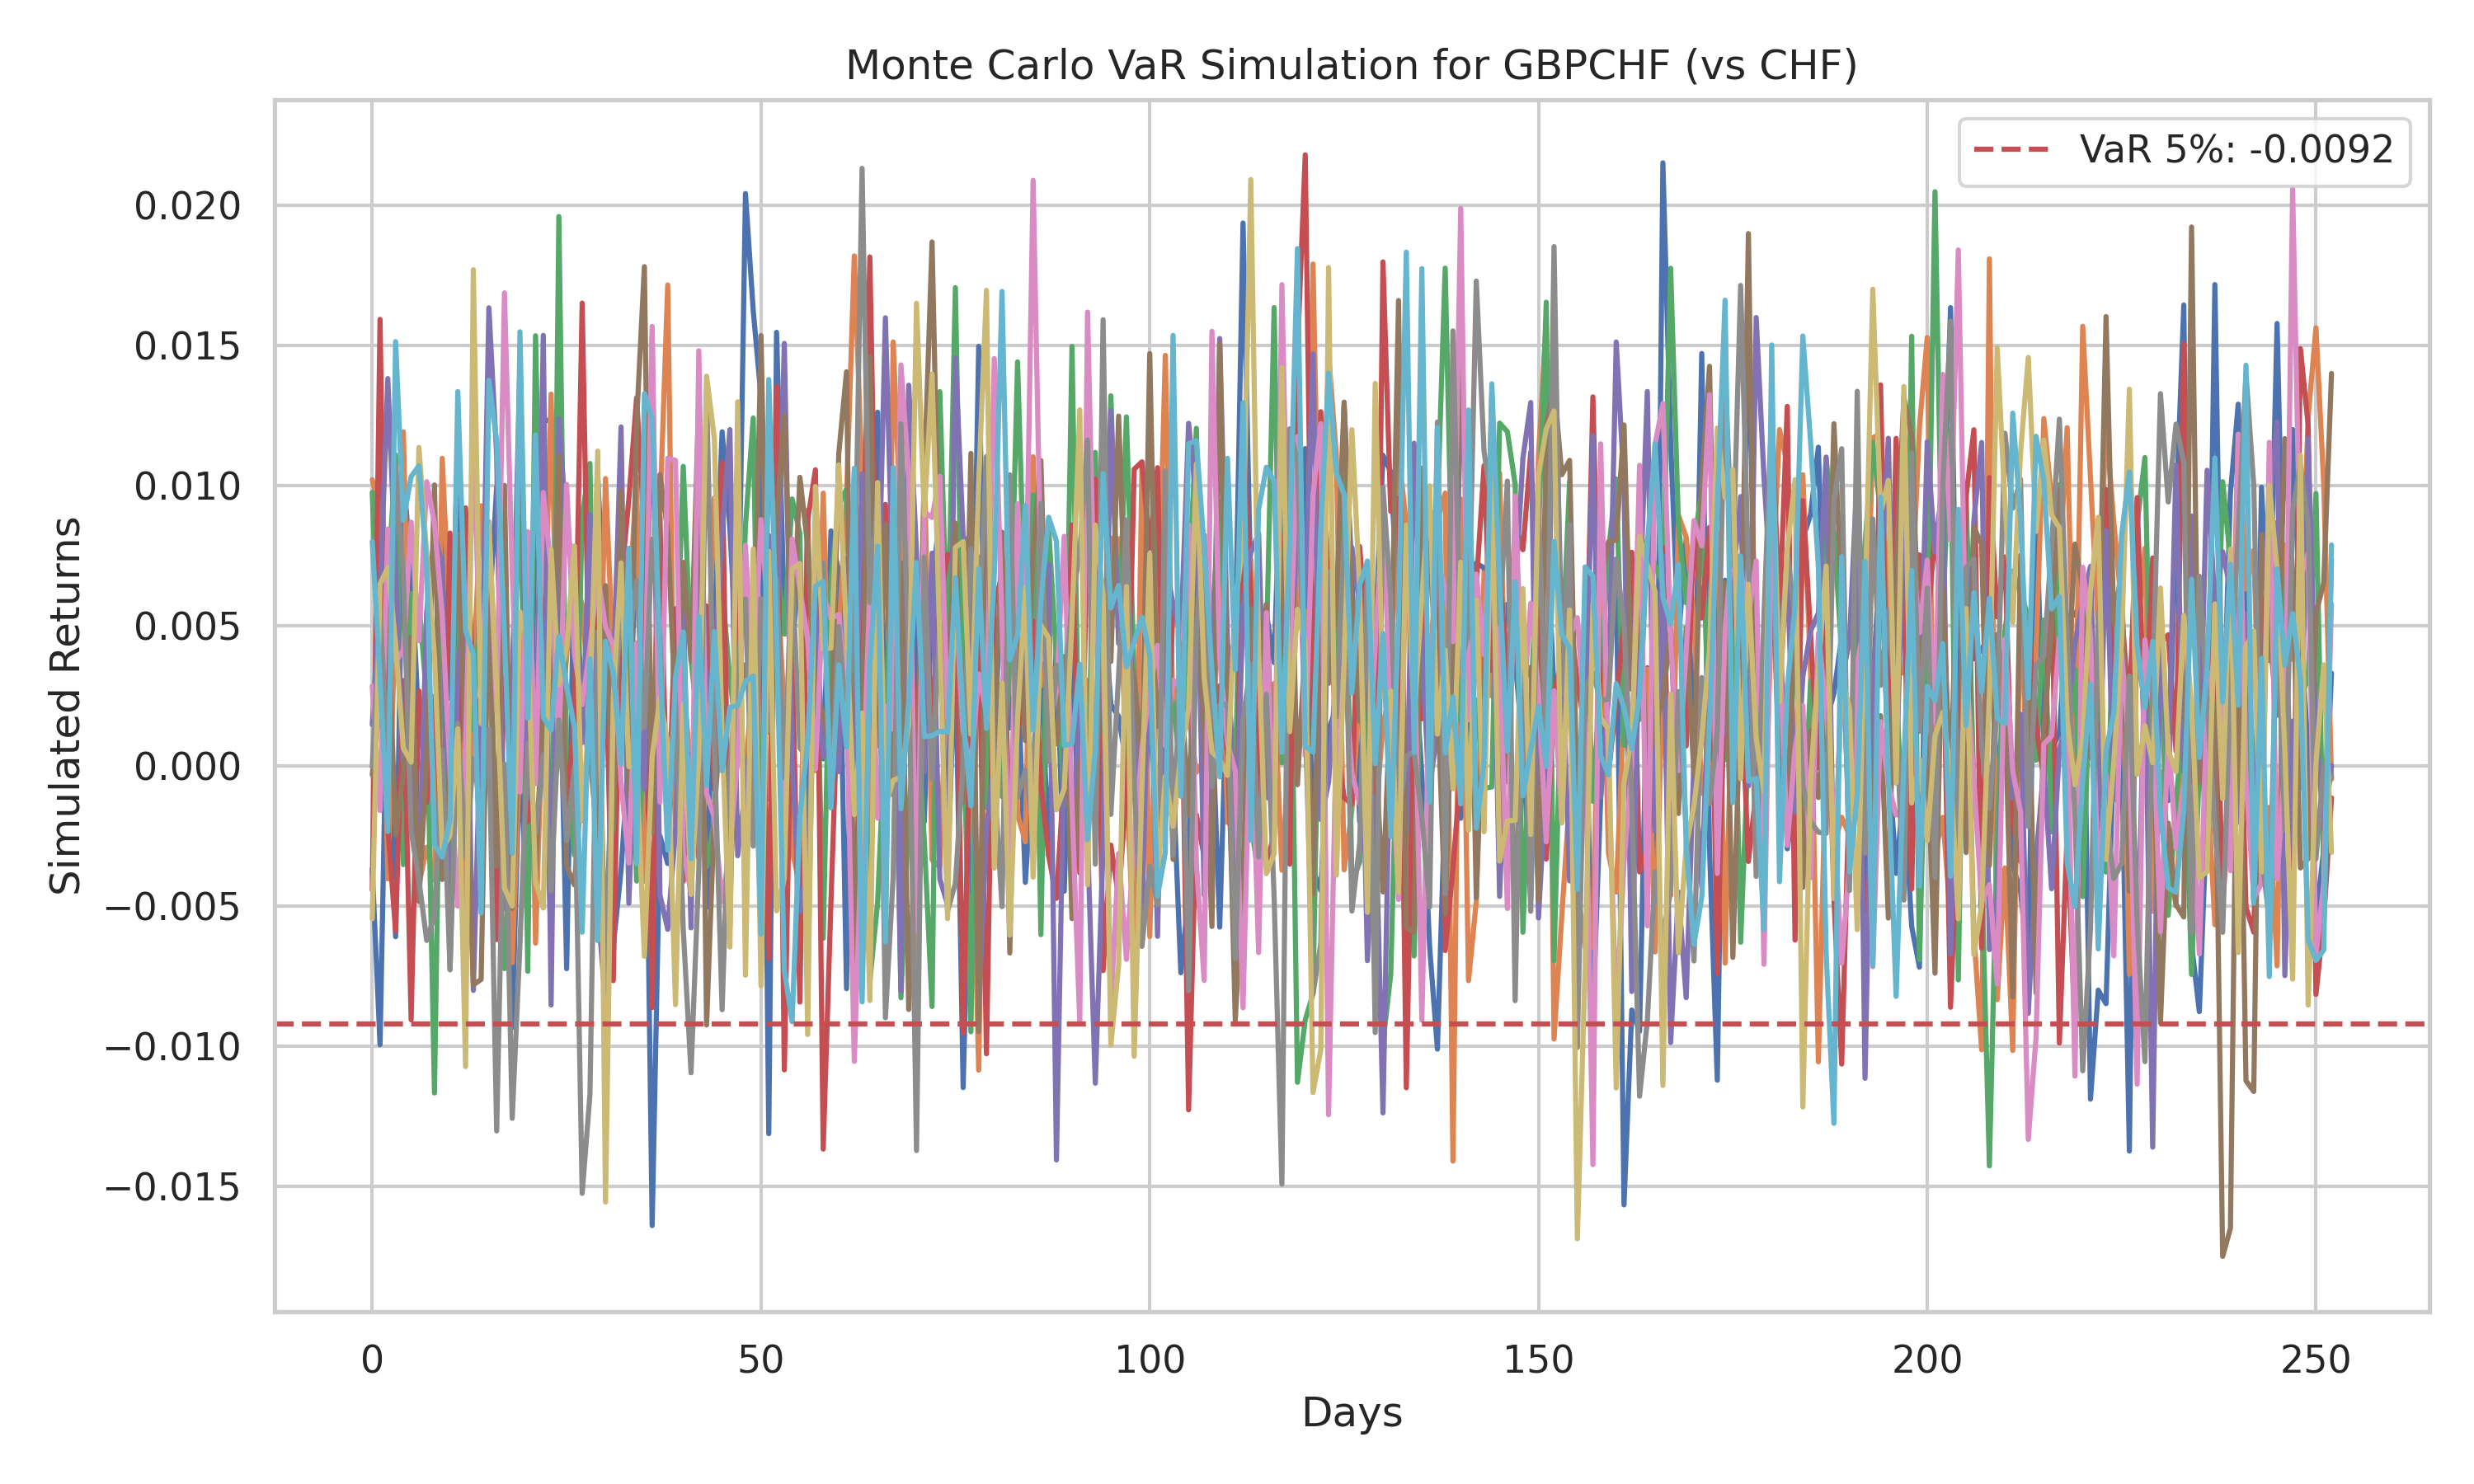
\includegraphics[width=0.48\linewidth]{reports/figures/monte_carlo_var_simulation_GBPCHF_vs_CHF.png} \label{fig:monte_carlo_var_simulation_GBPCHF_vs_CHF}
    \caption{\footnotesize Monte Carlo price siulation (left) and VaR simulation (right) for GBP-CHF.}
\end{figure}
\end{frame}
% ---------------------------------------------------------------------------
\begin{frame}
\frametitle{Main Findings}
\begin{figure}
    \centering  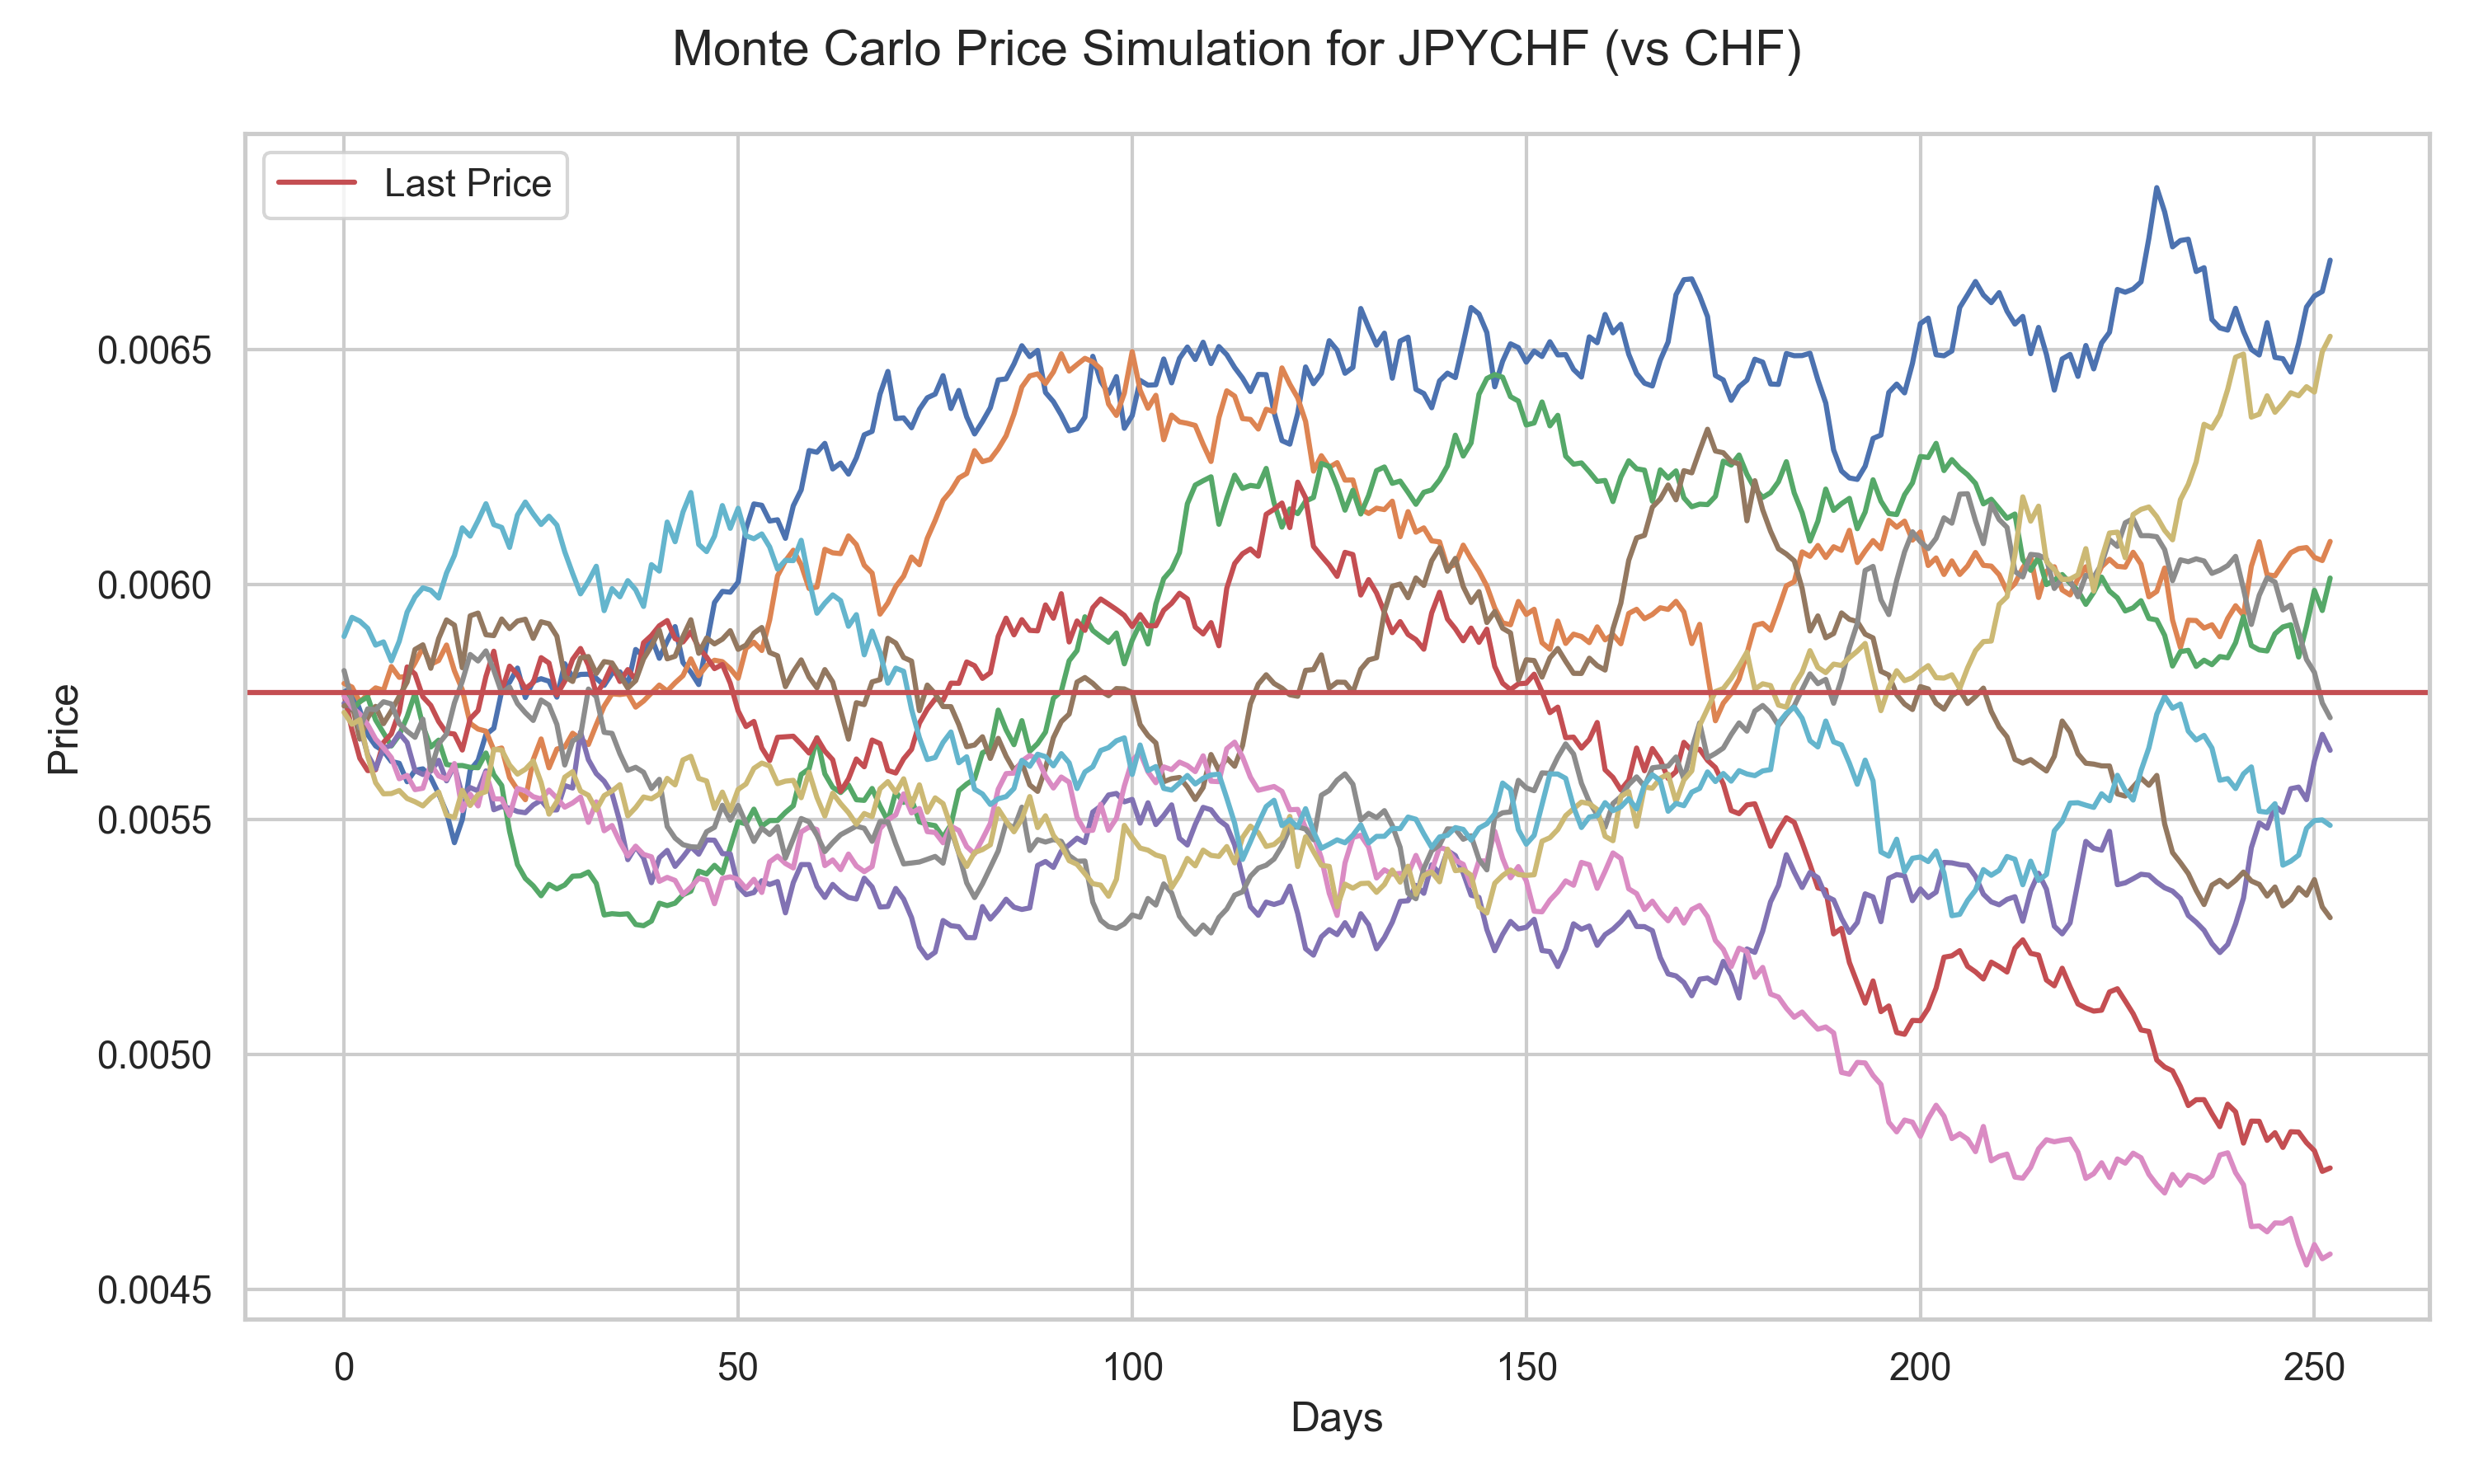
\includegraphics[width=0.48\linewidth]{reports/figures/monte_carlo_price_simulation_JPYCHF_vs_CHF.png}  \label{fig:monte_carlo_price_simulation_JPYCHF_vs_CHF}
    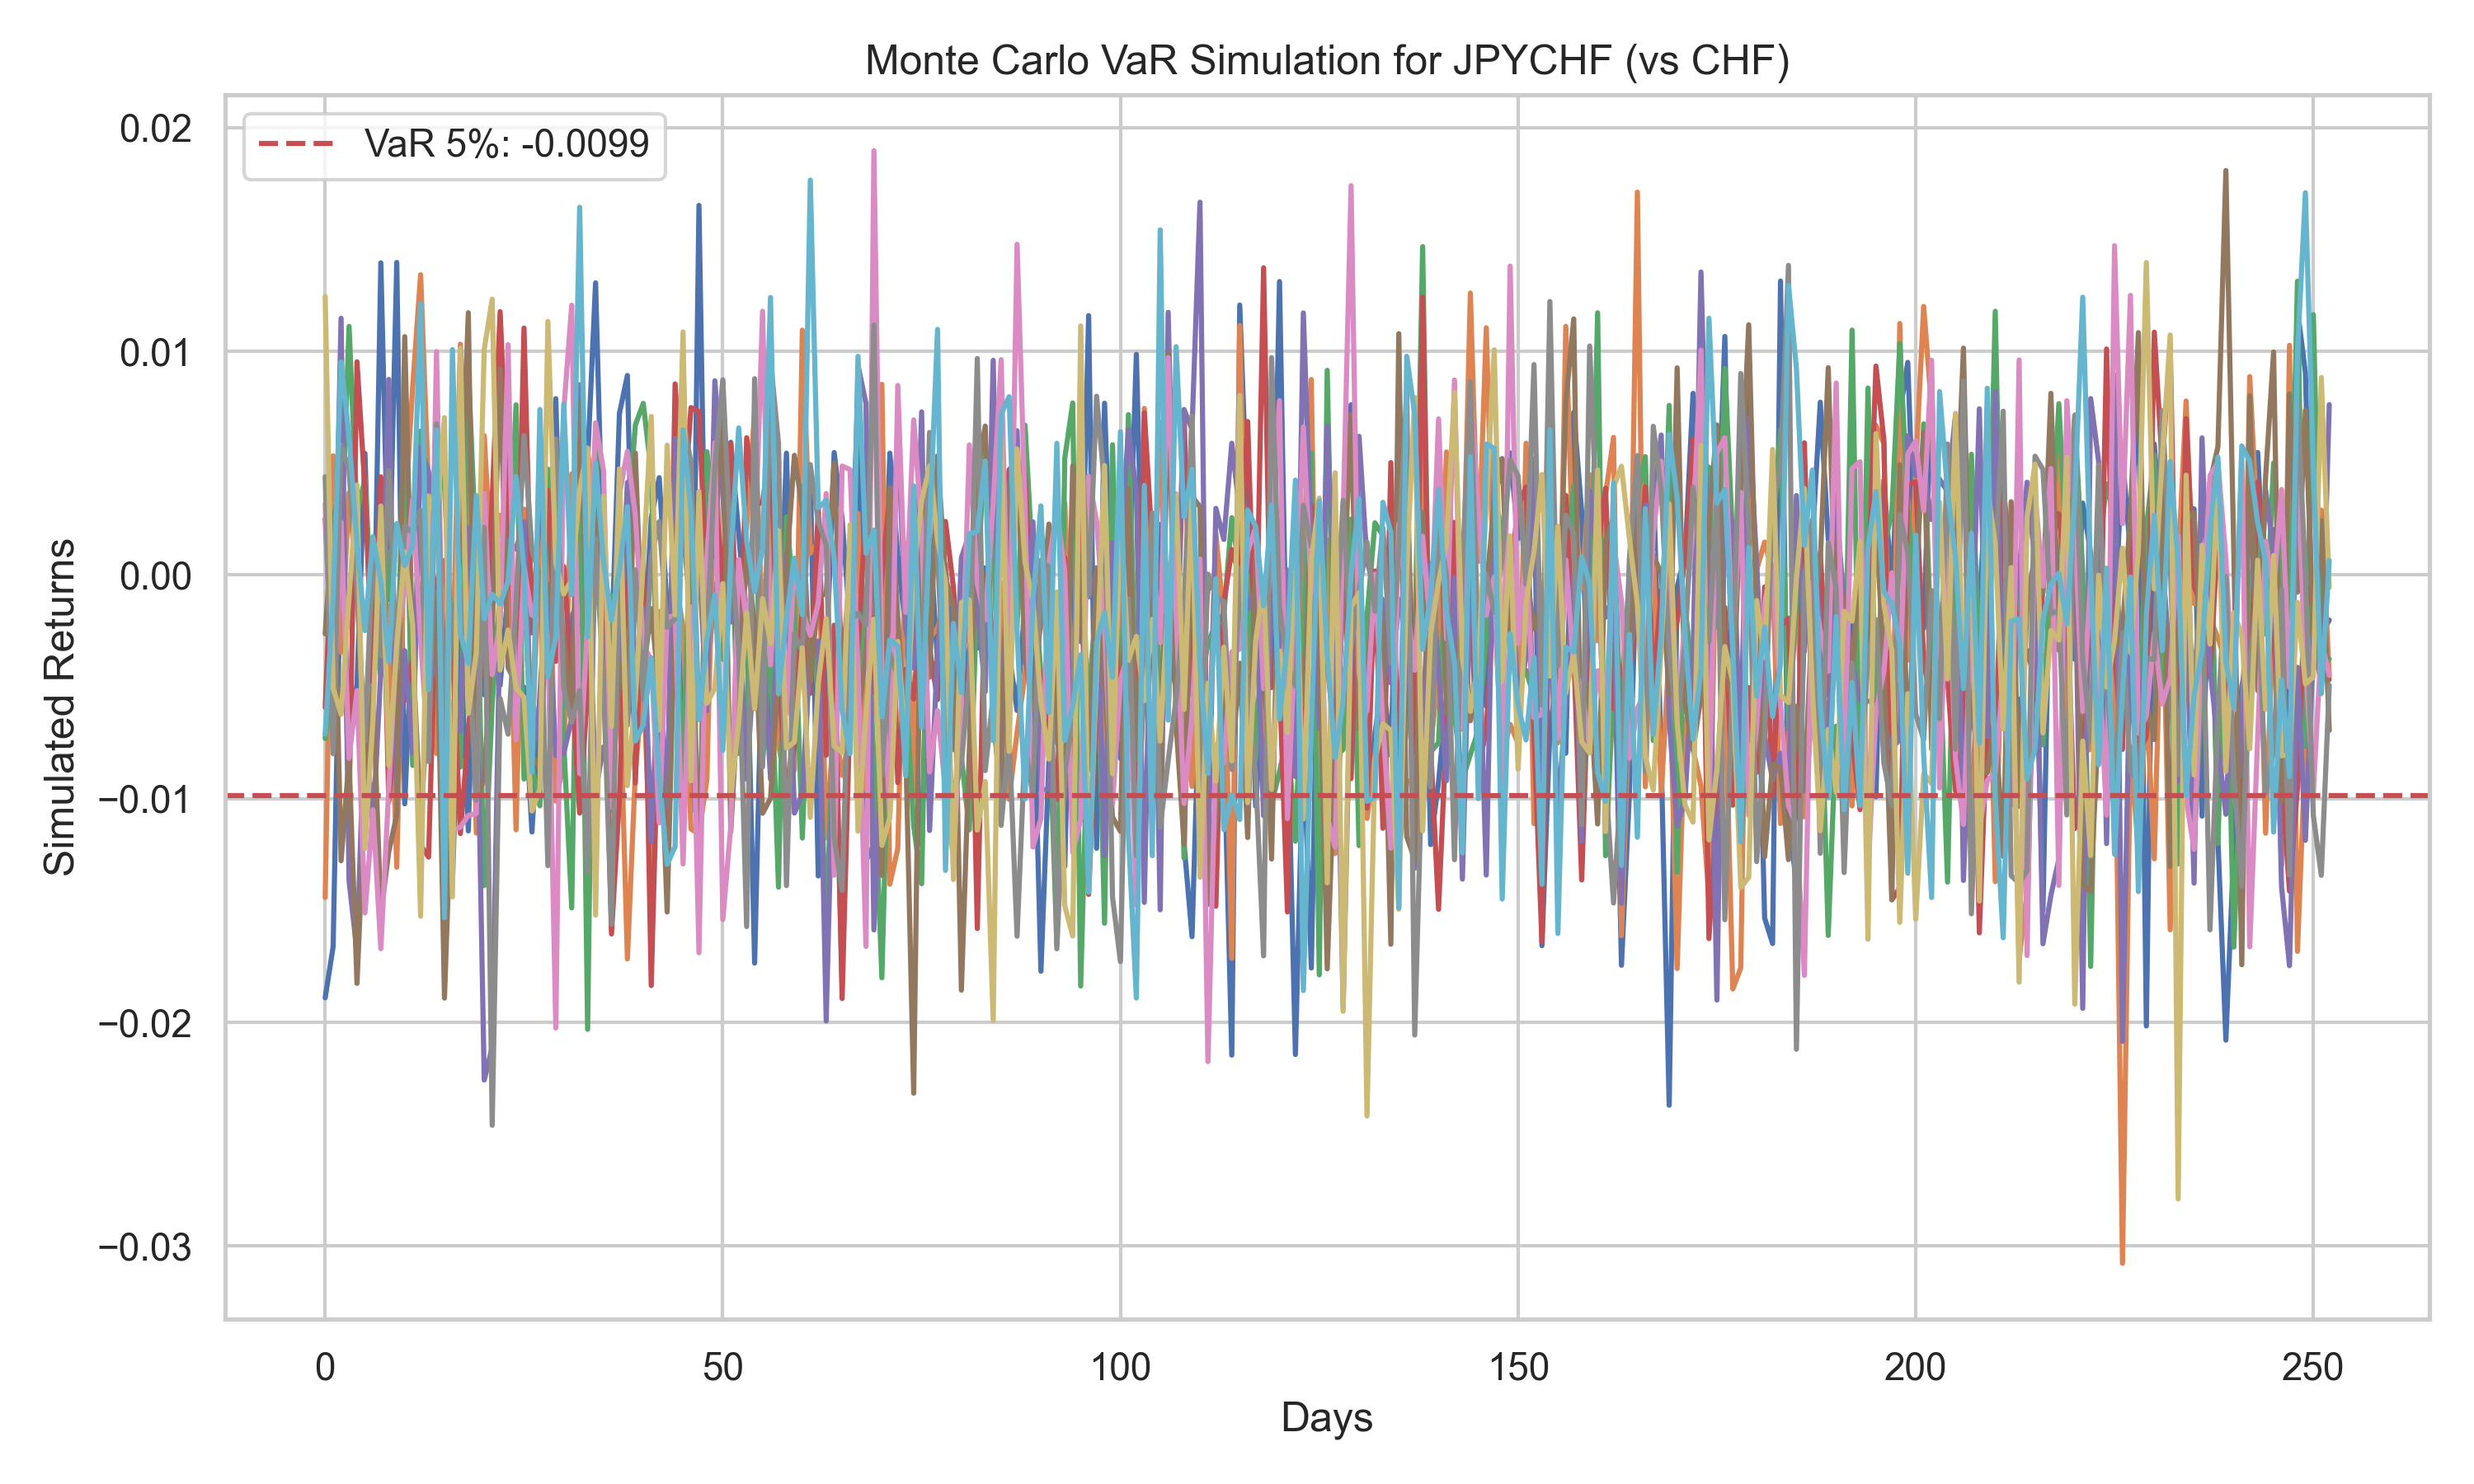
\includegraphics[width=0.48\linewidth]{reports/figures/monte_carlo_var_simulation_JPYCHF_vs_CHF.png}  \label{fig:monte_carlo_var_simulation_JPYCHF_vs_CHF}
    \caption{\footnotesize Monte Carlo price siulation (left) and VaR simulation (right) for JPY-CHF.}
\end{figure}
\begin{figure}
    \centering   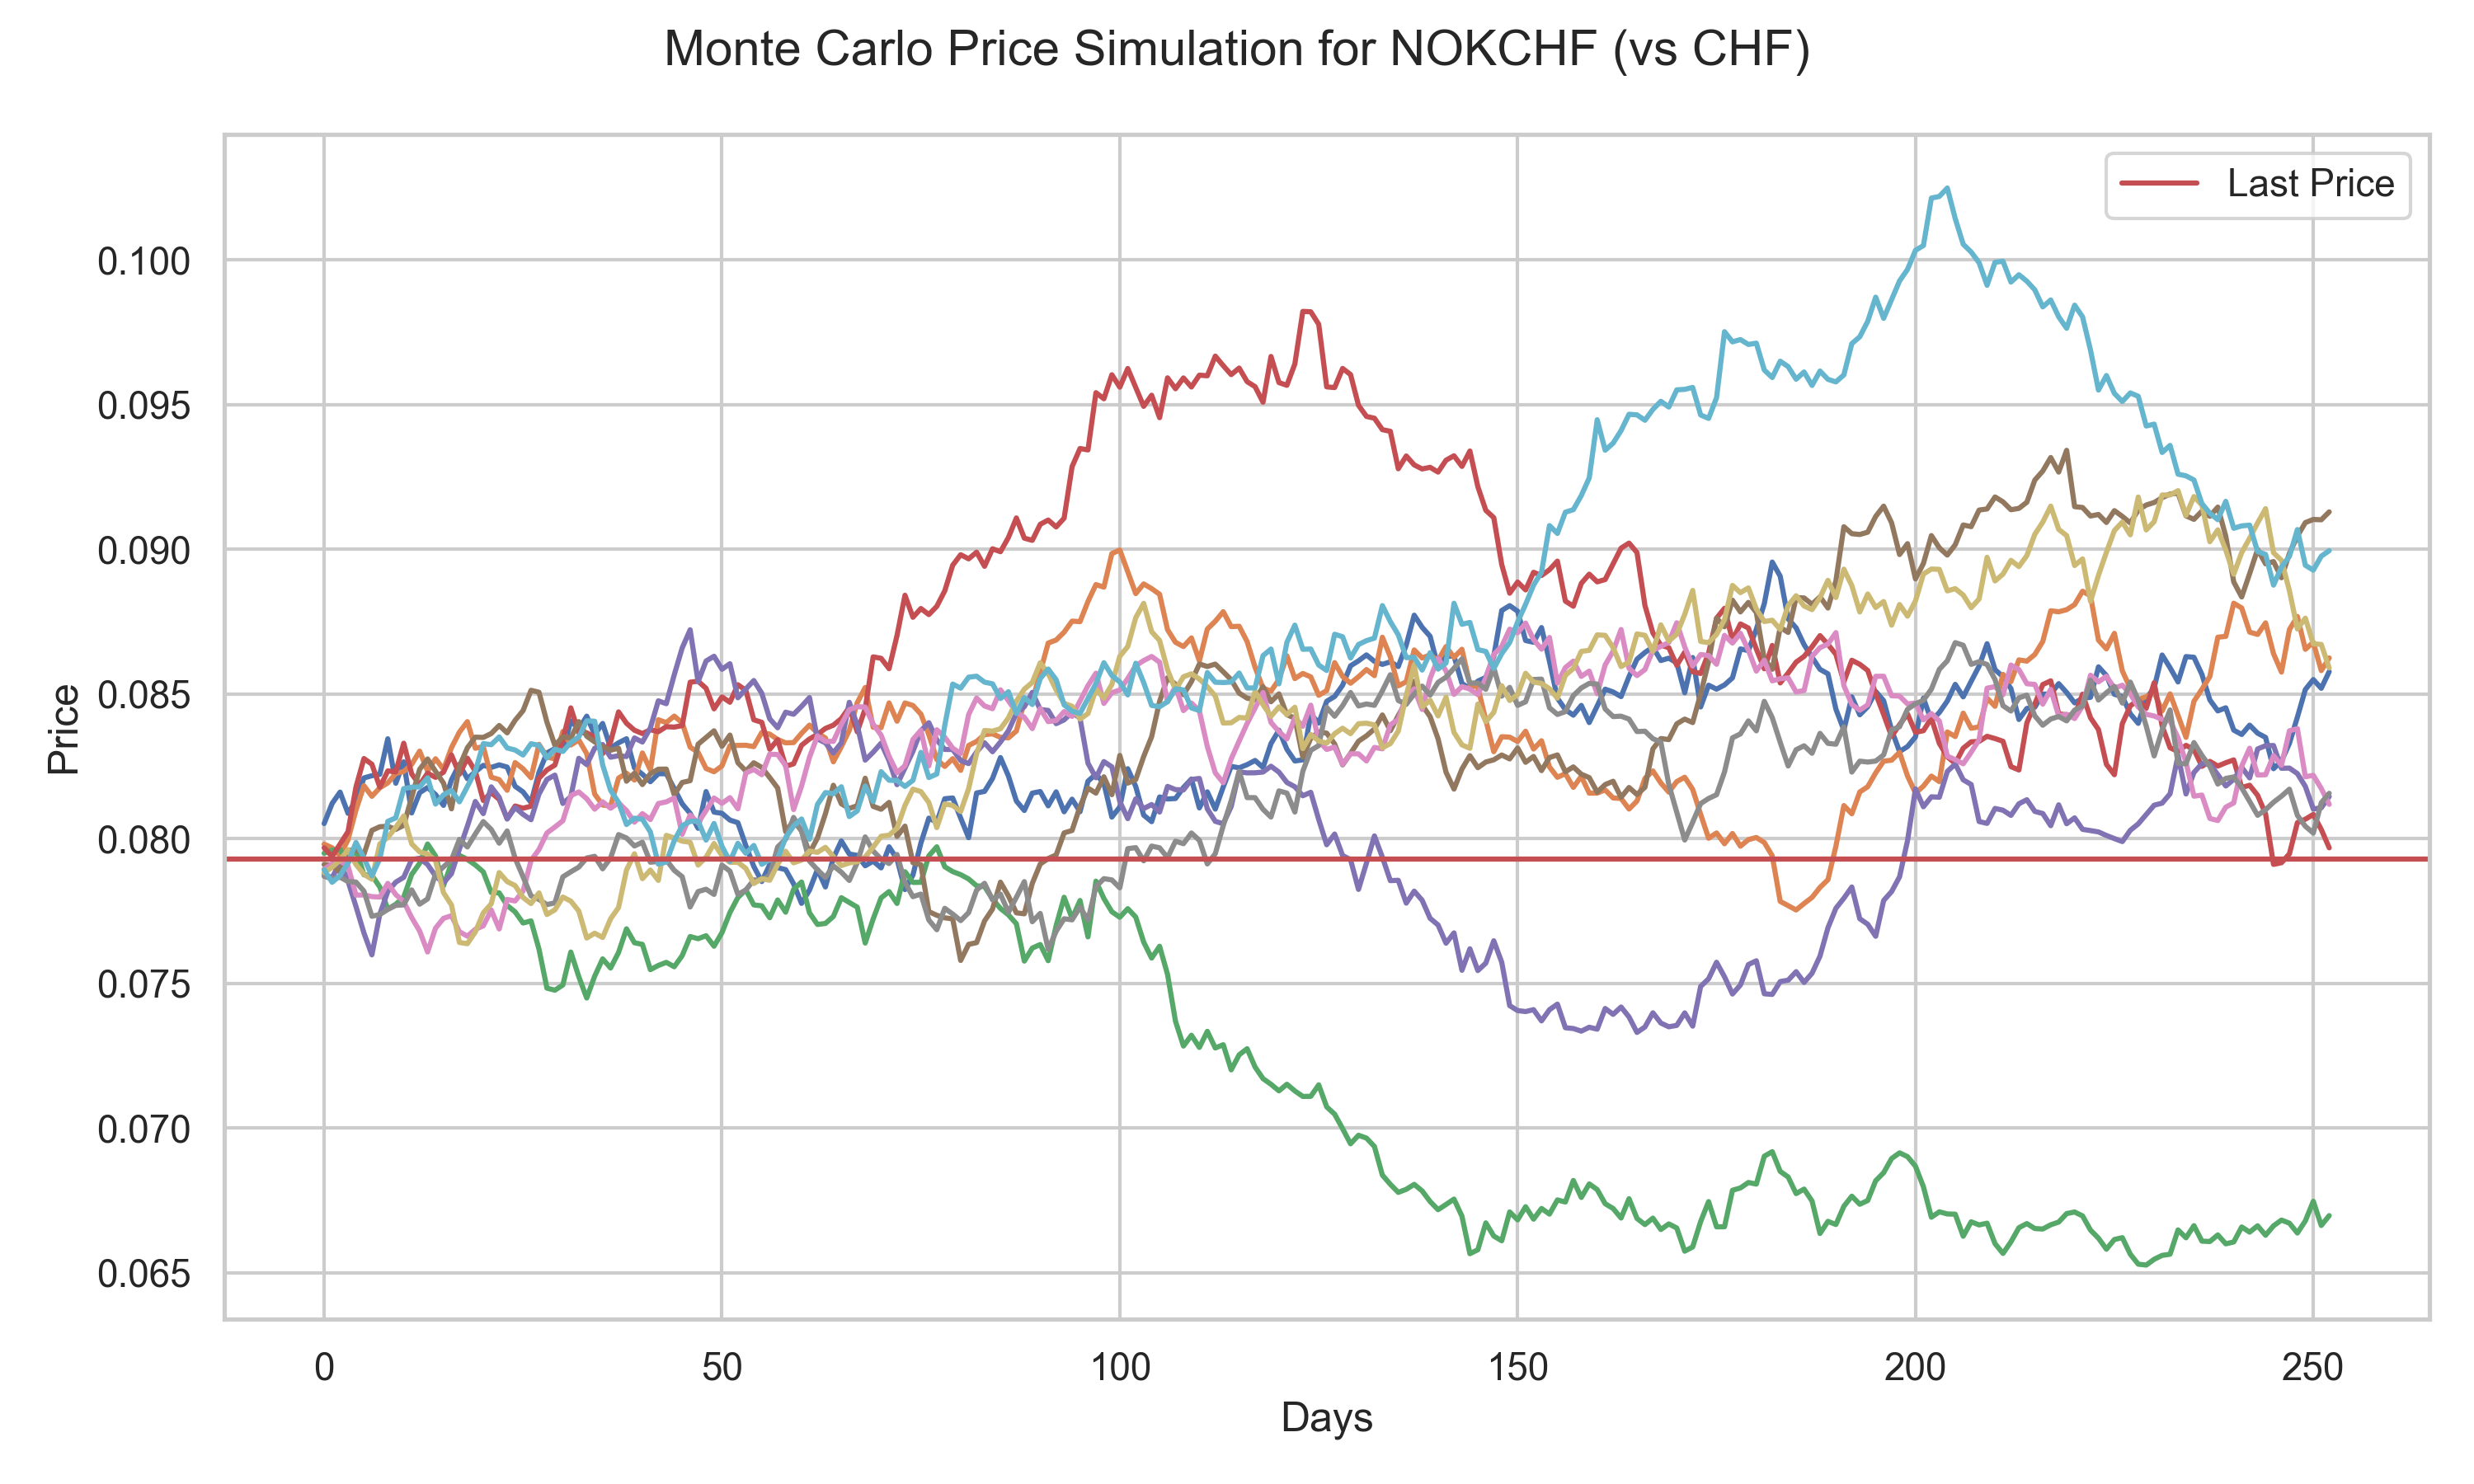
\includegraphics[width=0.48\linewidth]{reports/figures/monte_carlo_price_simulation_NOKCHF_vs_CHF.png} \label{fig:monte_carlo_price_simulation_NOKCHF_vs_CHF}
    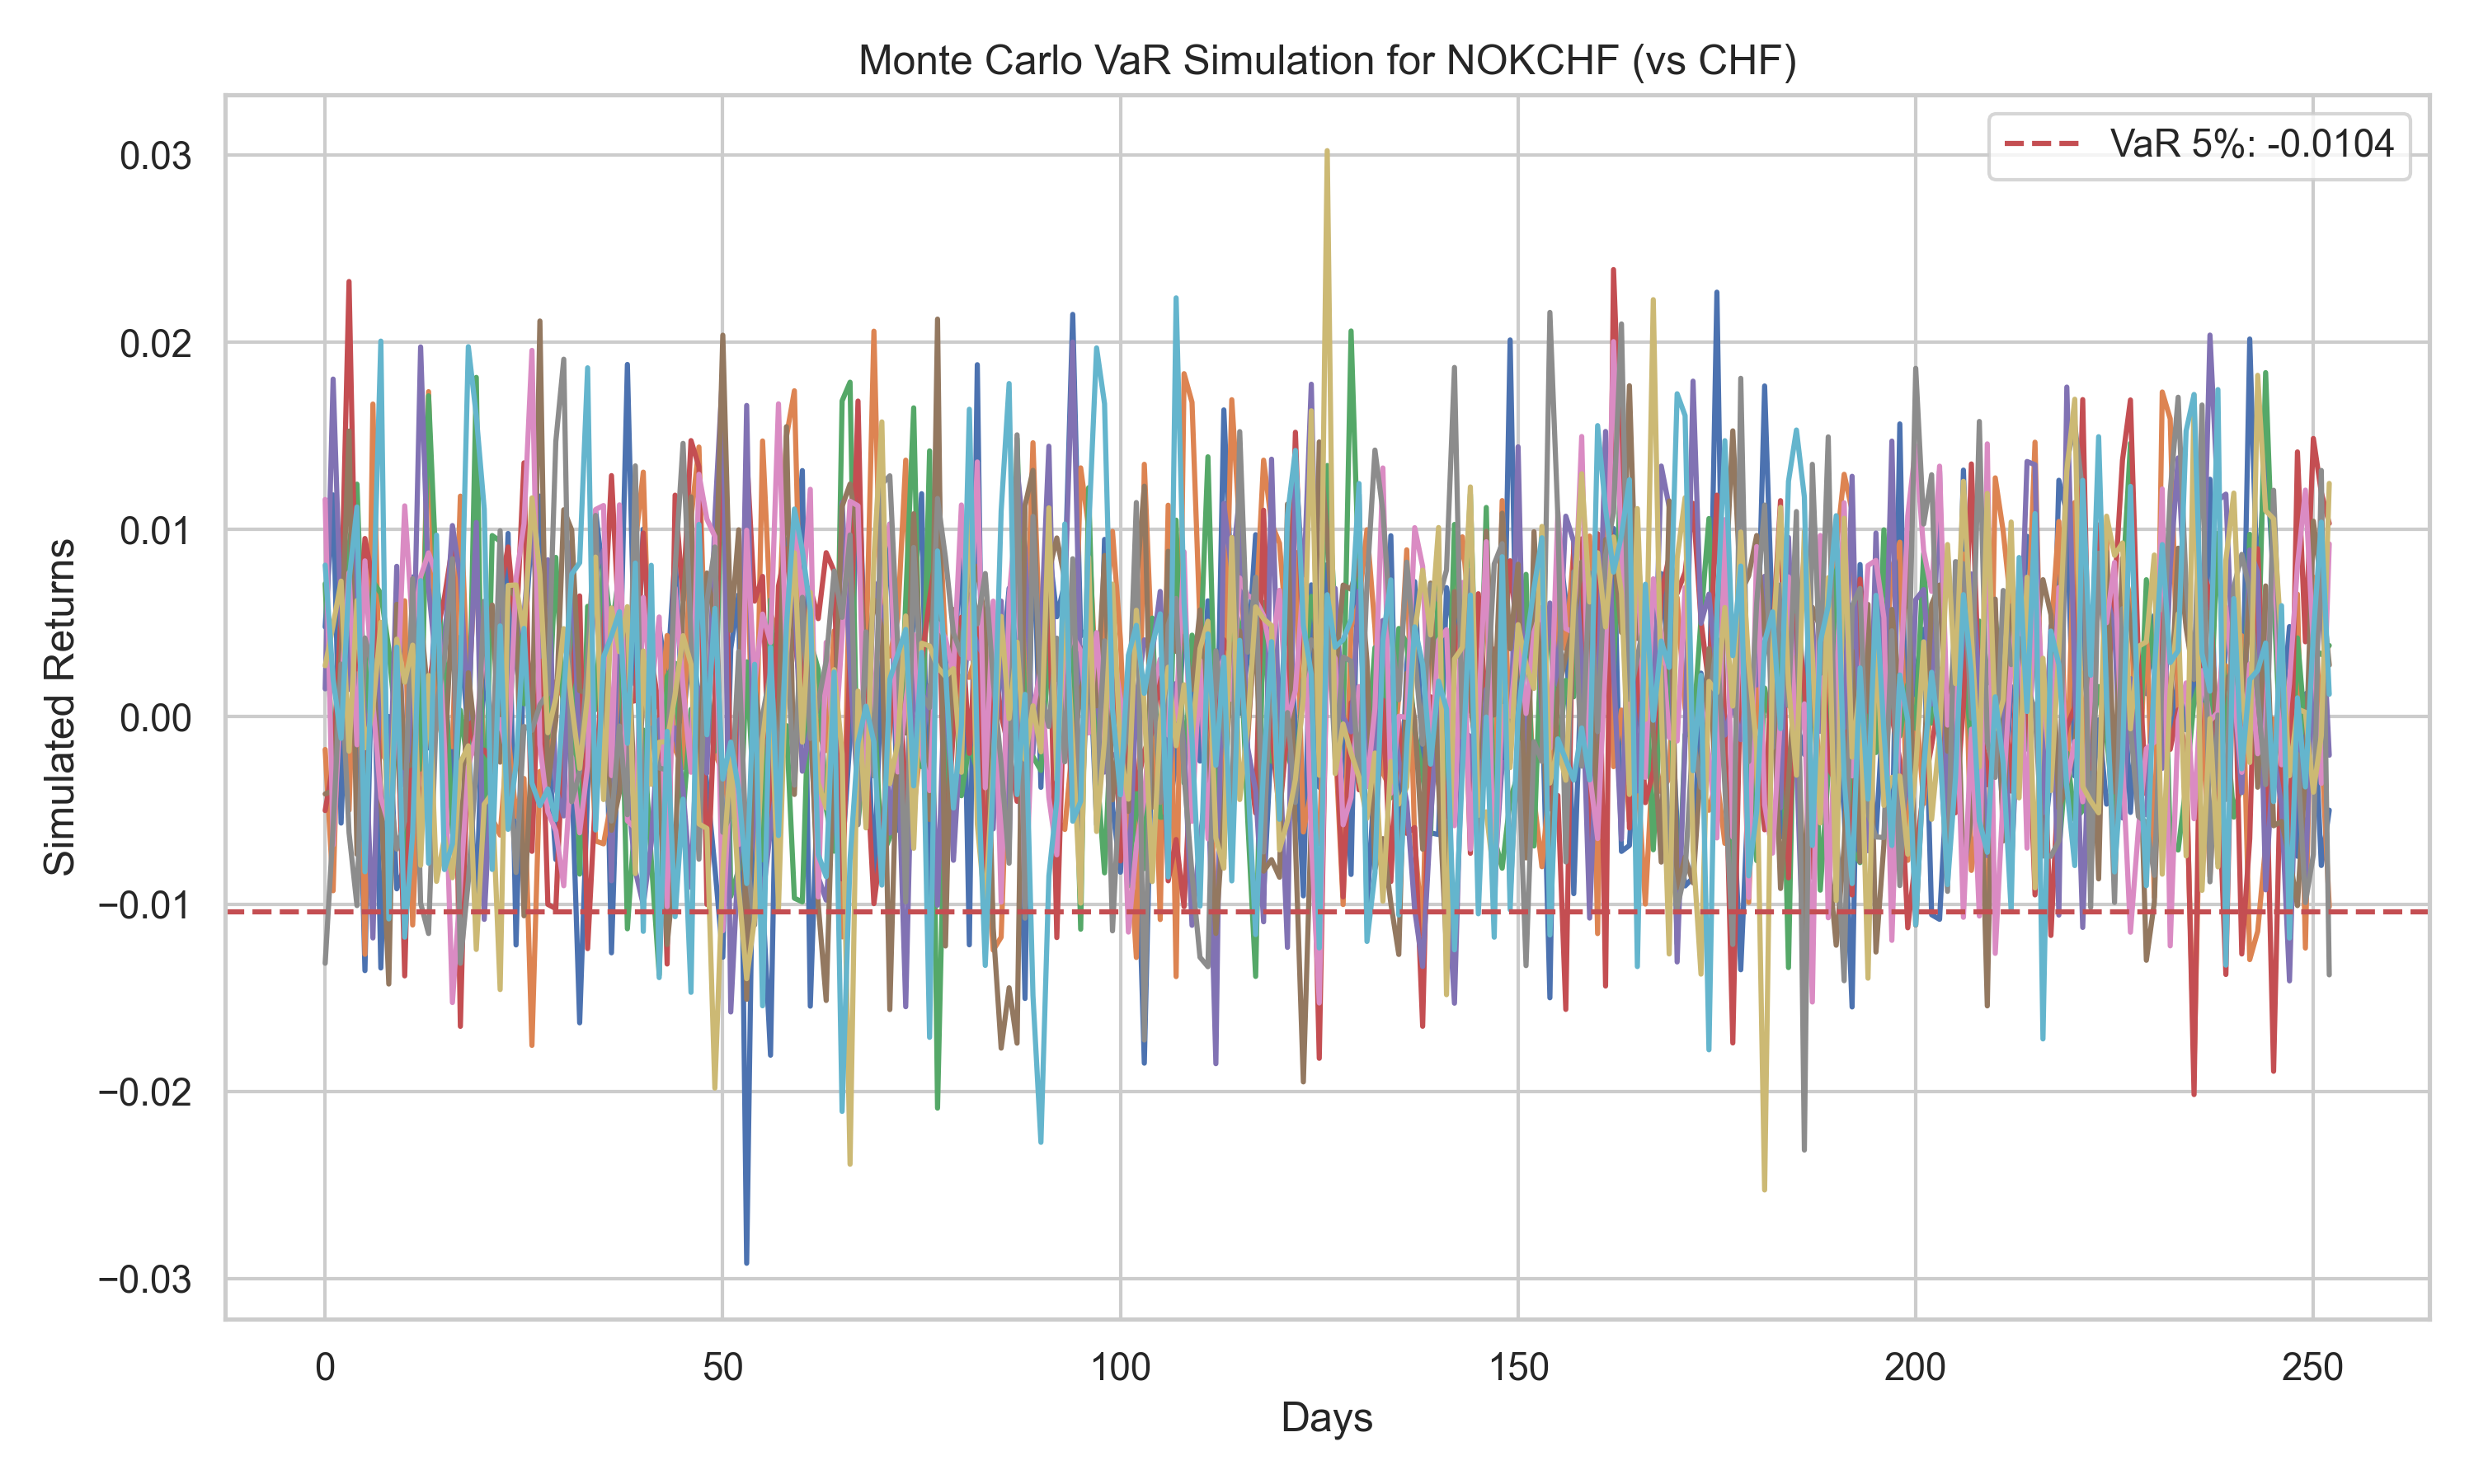
\includegraphics[width=0.48\linewidth]{reports/figures/monte_carlo_var_simulation_NOKCHF_vs_CHF.png} \label{fig:monte_carlo_var_simulation_NOKCHF_vs_CHF}
    \caption{\footnotesize Monte Carlo price siulation (left) and VaR simulation (right) for NOK-CHF.}
\end{figure}
\end{frame}
% ---------------------------------------------------------------------------
\begin{frame}
\frametitle{Main Findings}
\begin{figure}
    \centering  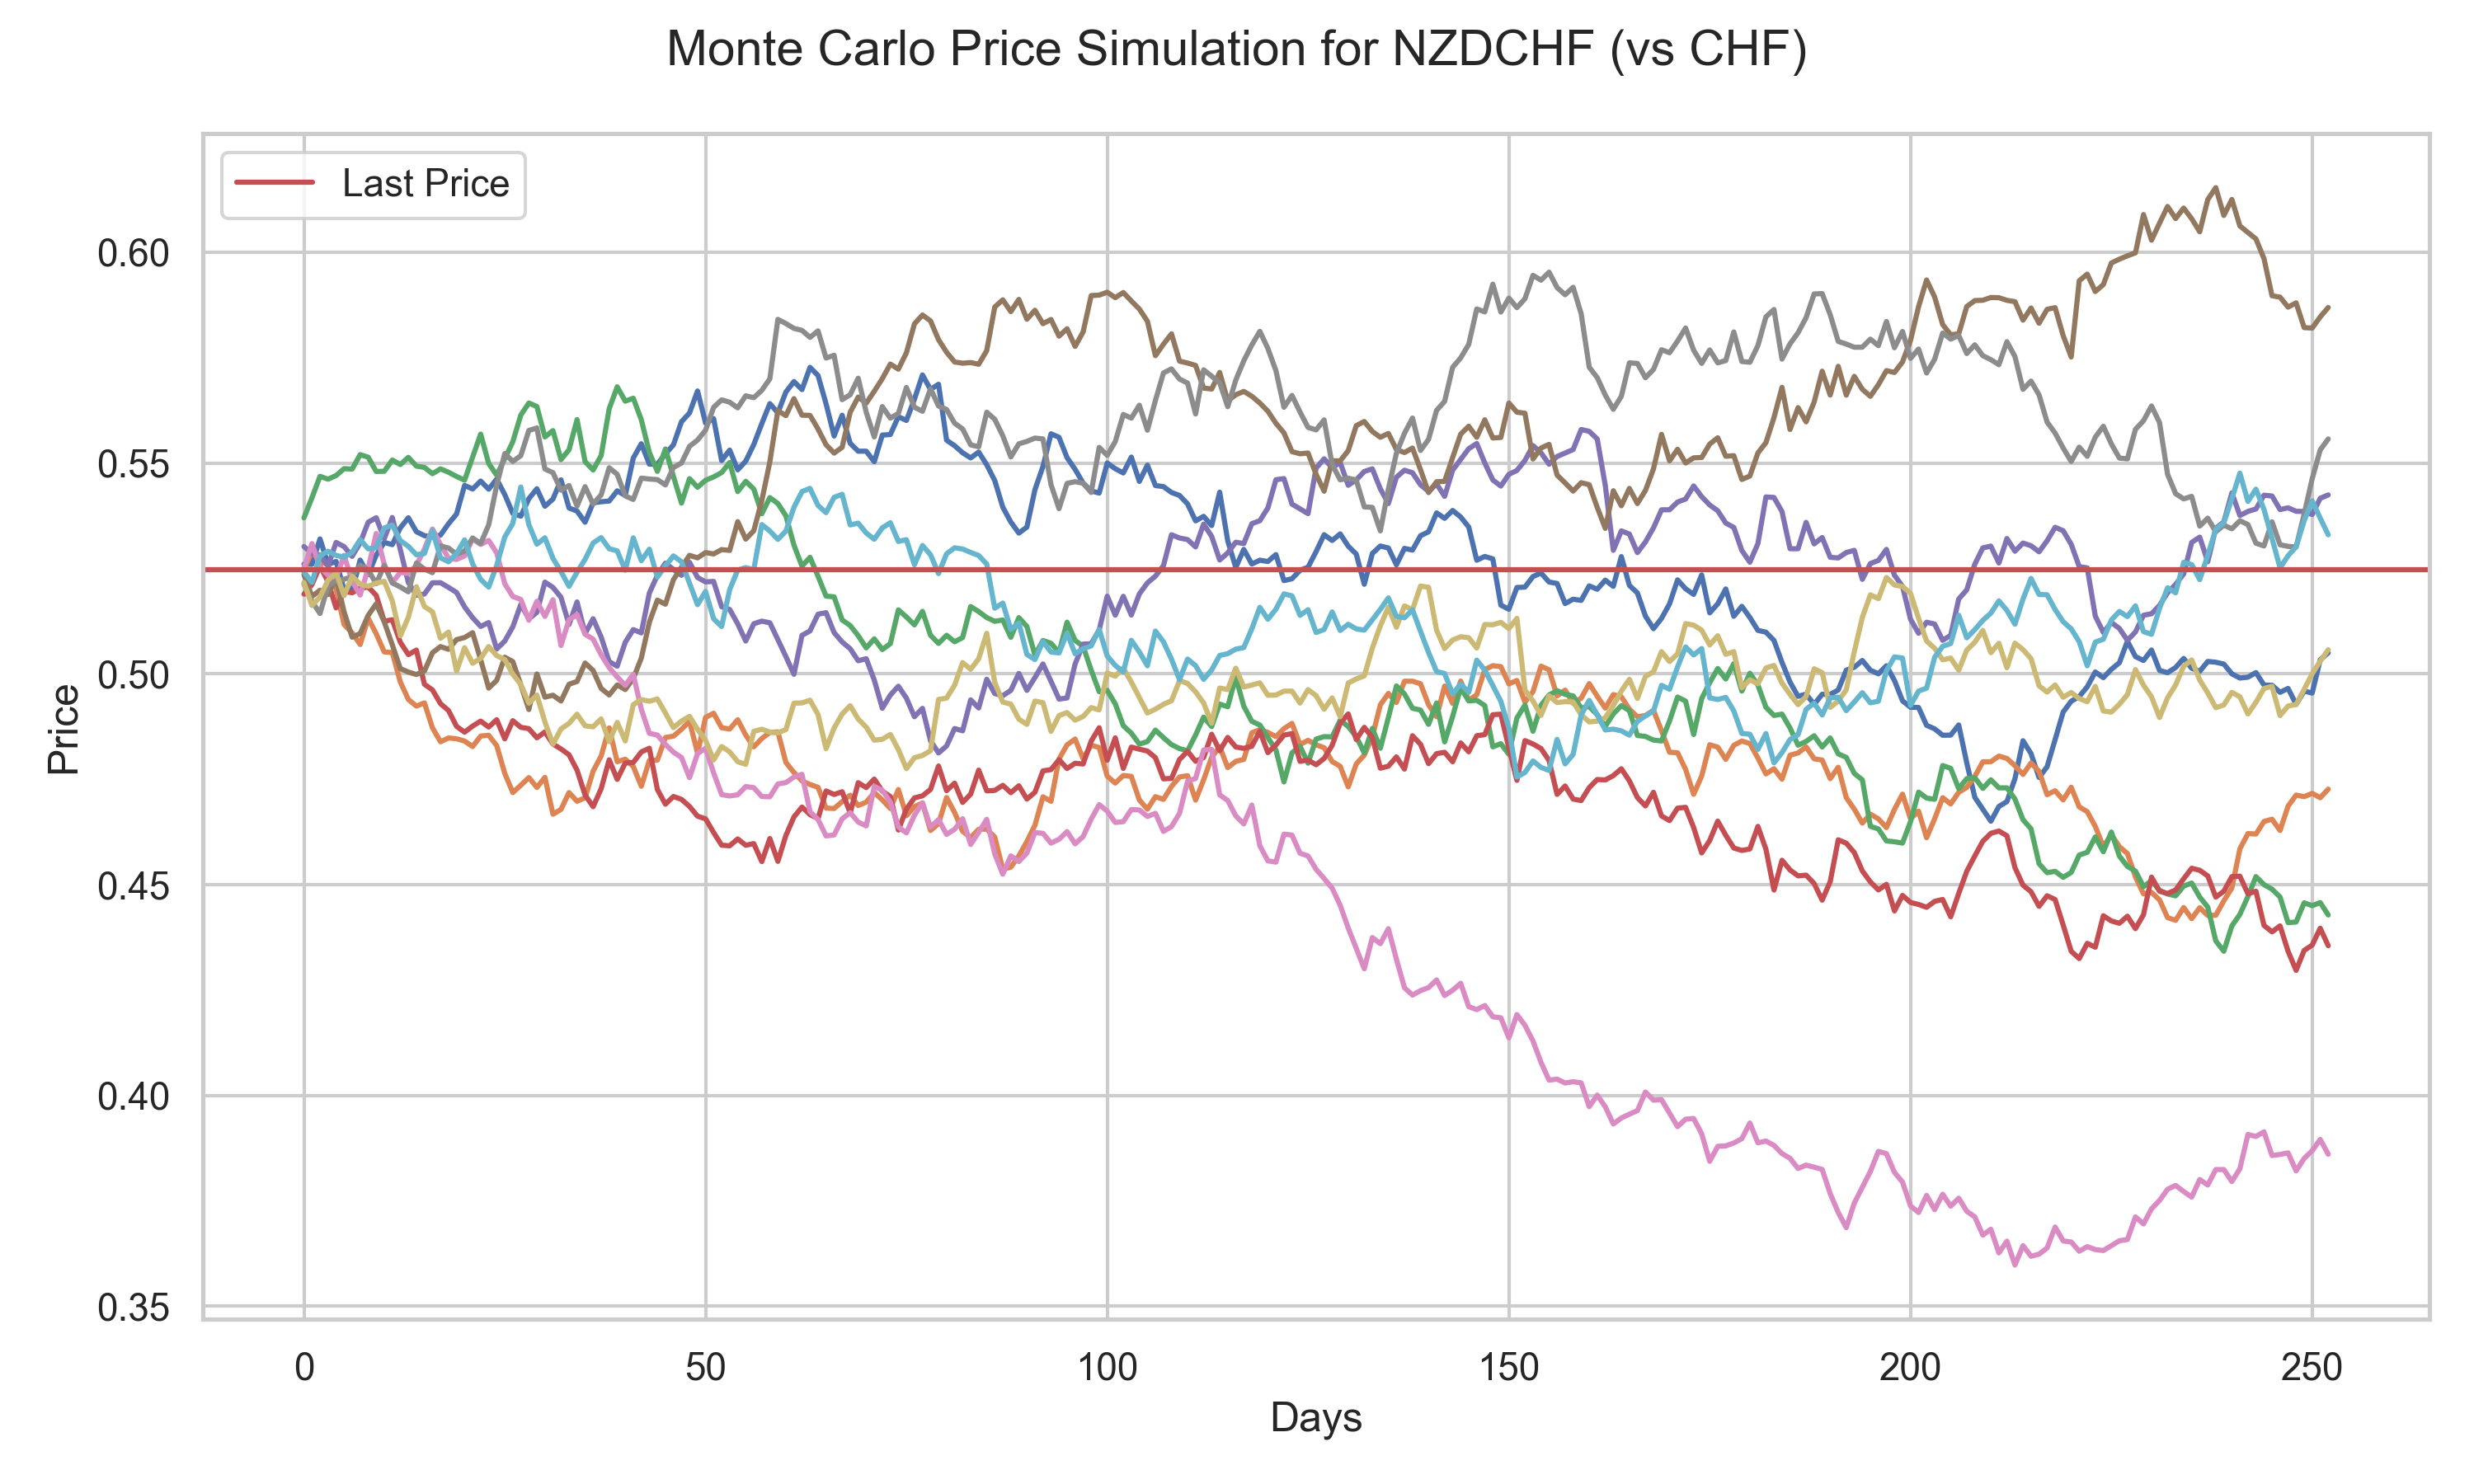
\includegraphics[width=0.48\linewidth]{reports/figures/monte_carlo_price_simulation_NZDCHF_vs_CHF.png}  \label{fig:monte_carlo_price_simulation_NZDCHF_vs_CHF}
    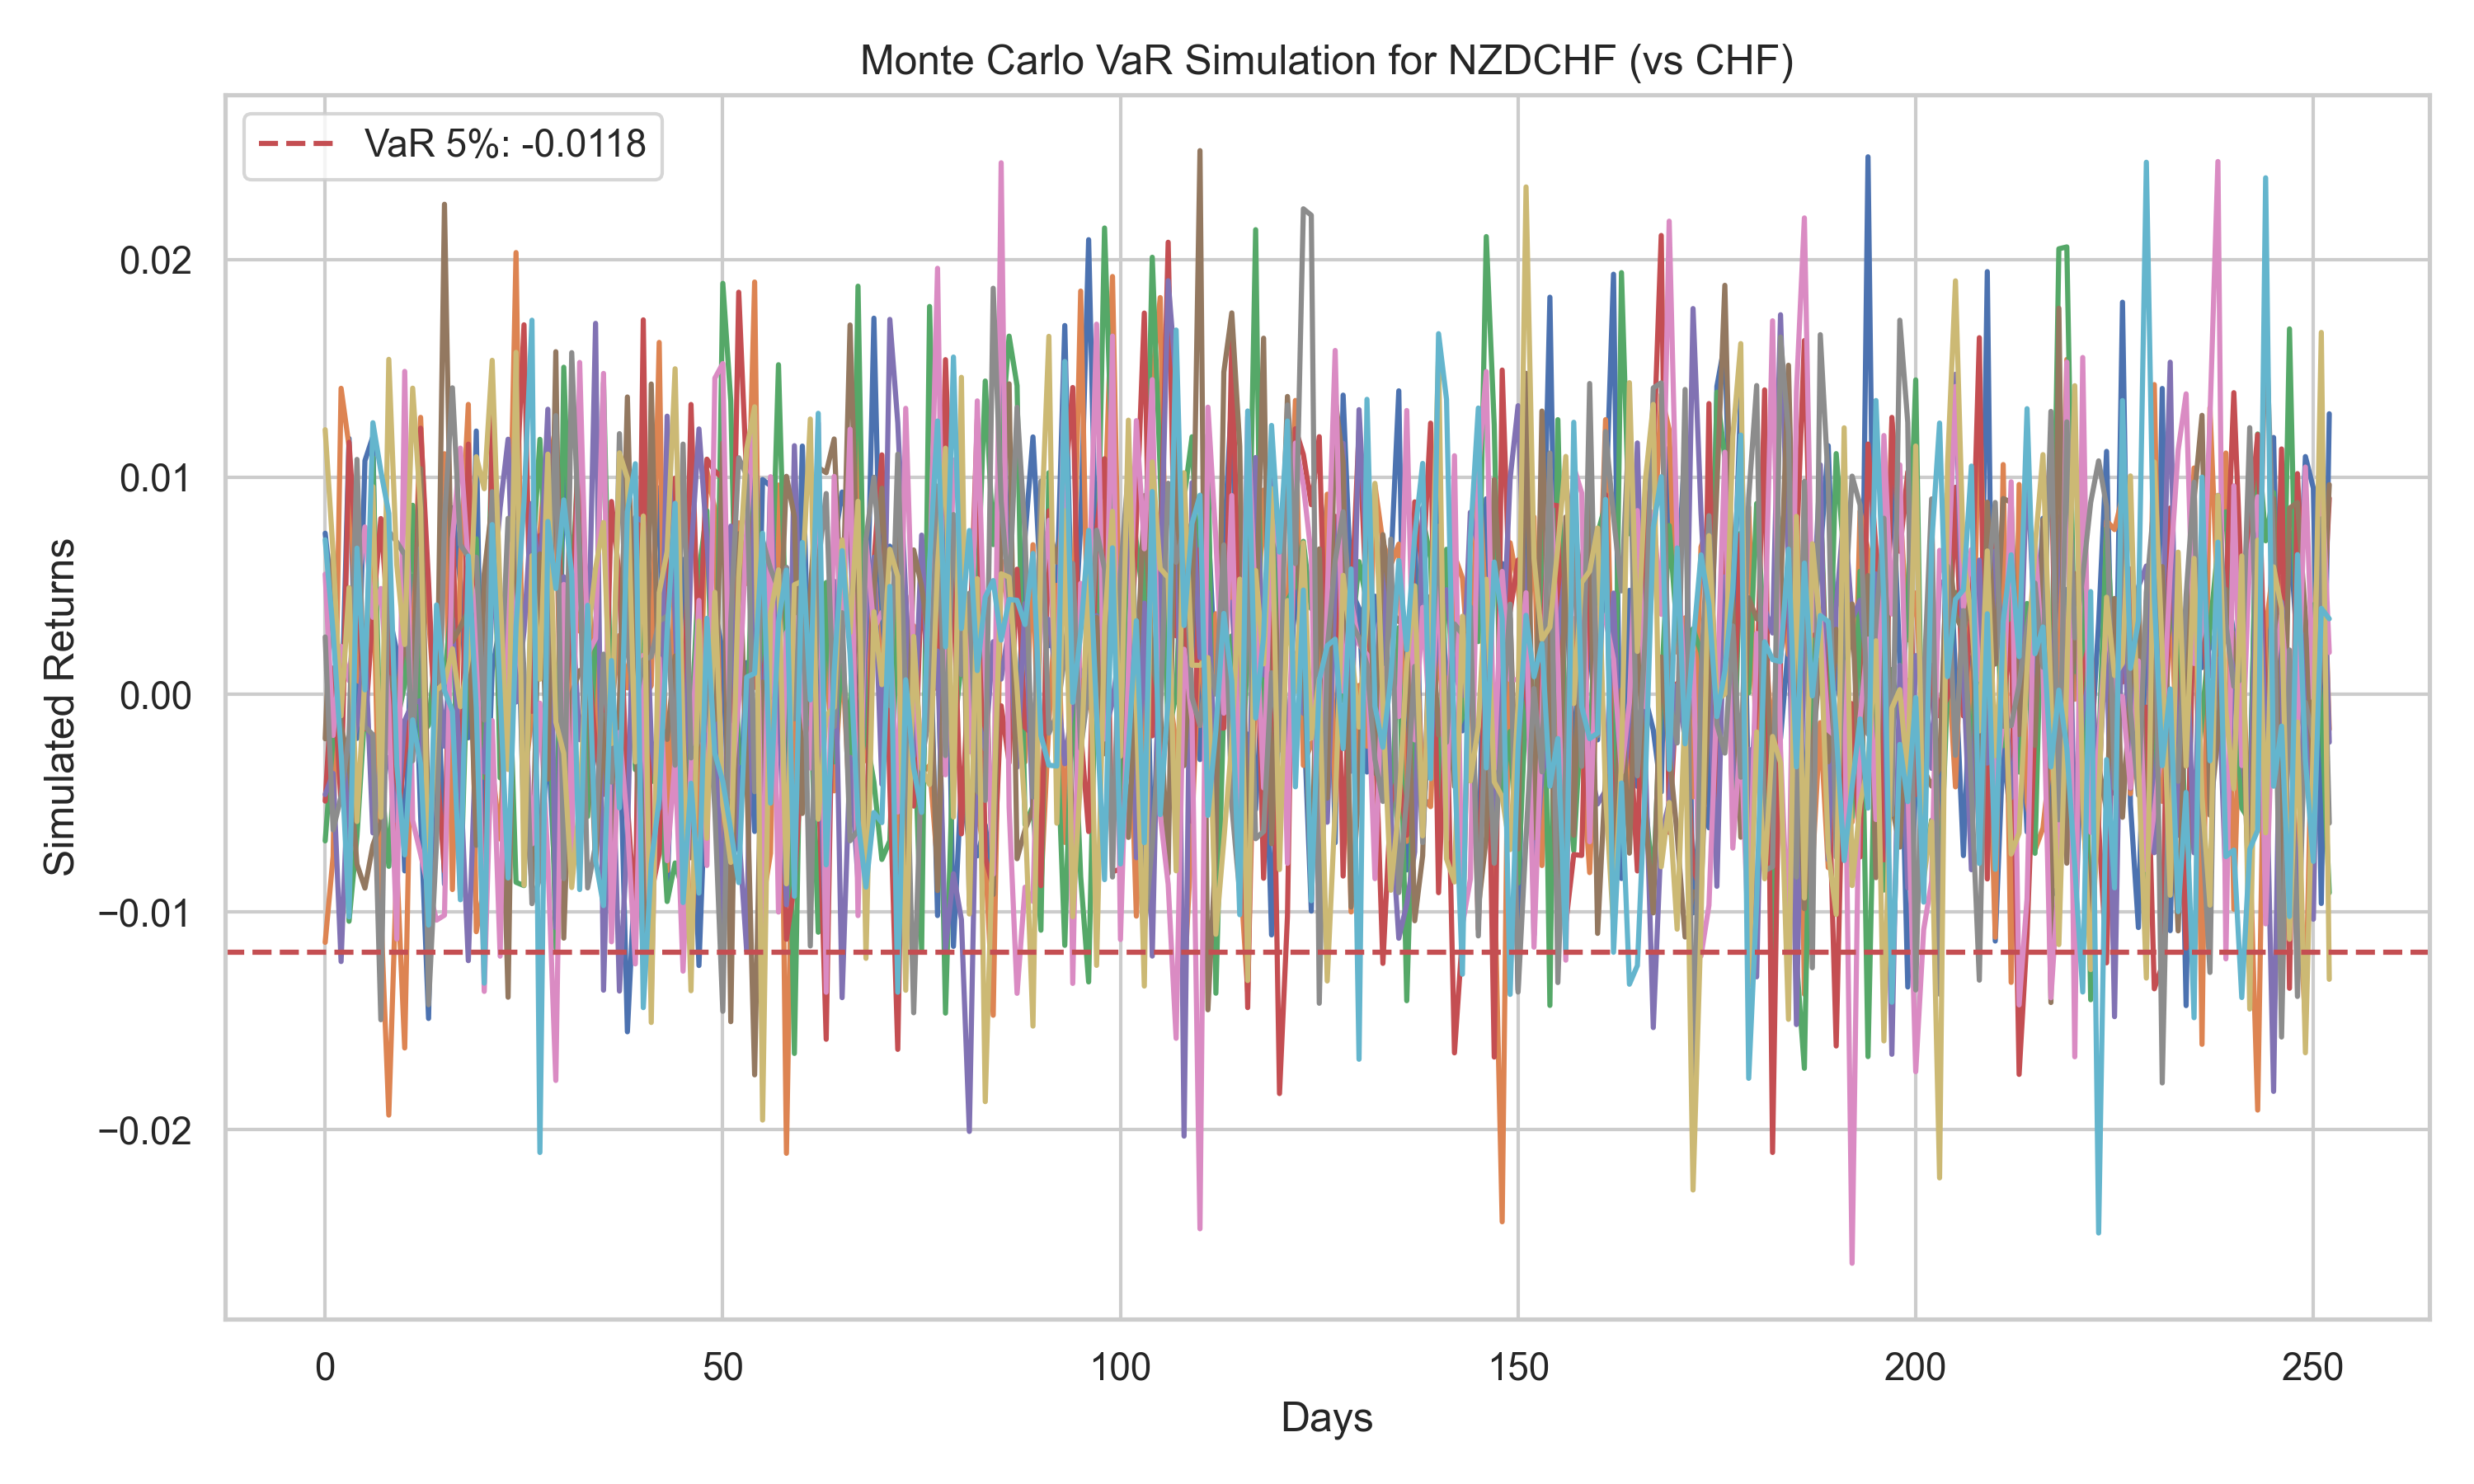
\includegraphics[width=0.48\linewidth]{reports/figures/monte_carlo_var_simulation_NZDCHF_vs_CHF.png}  \label{fig:monte_carlo_var_simulation_NZDCHF_vs_CHF}
    \caption{\footnotesize Monte Carlo price siulation (left) and VaR simulation (right) for NZD-CHF.}
\end{figure}
\begin{figure}
    \centering   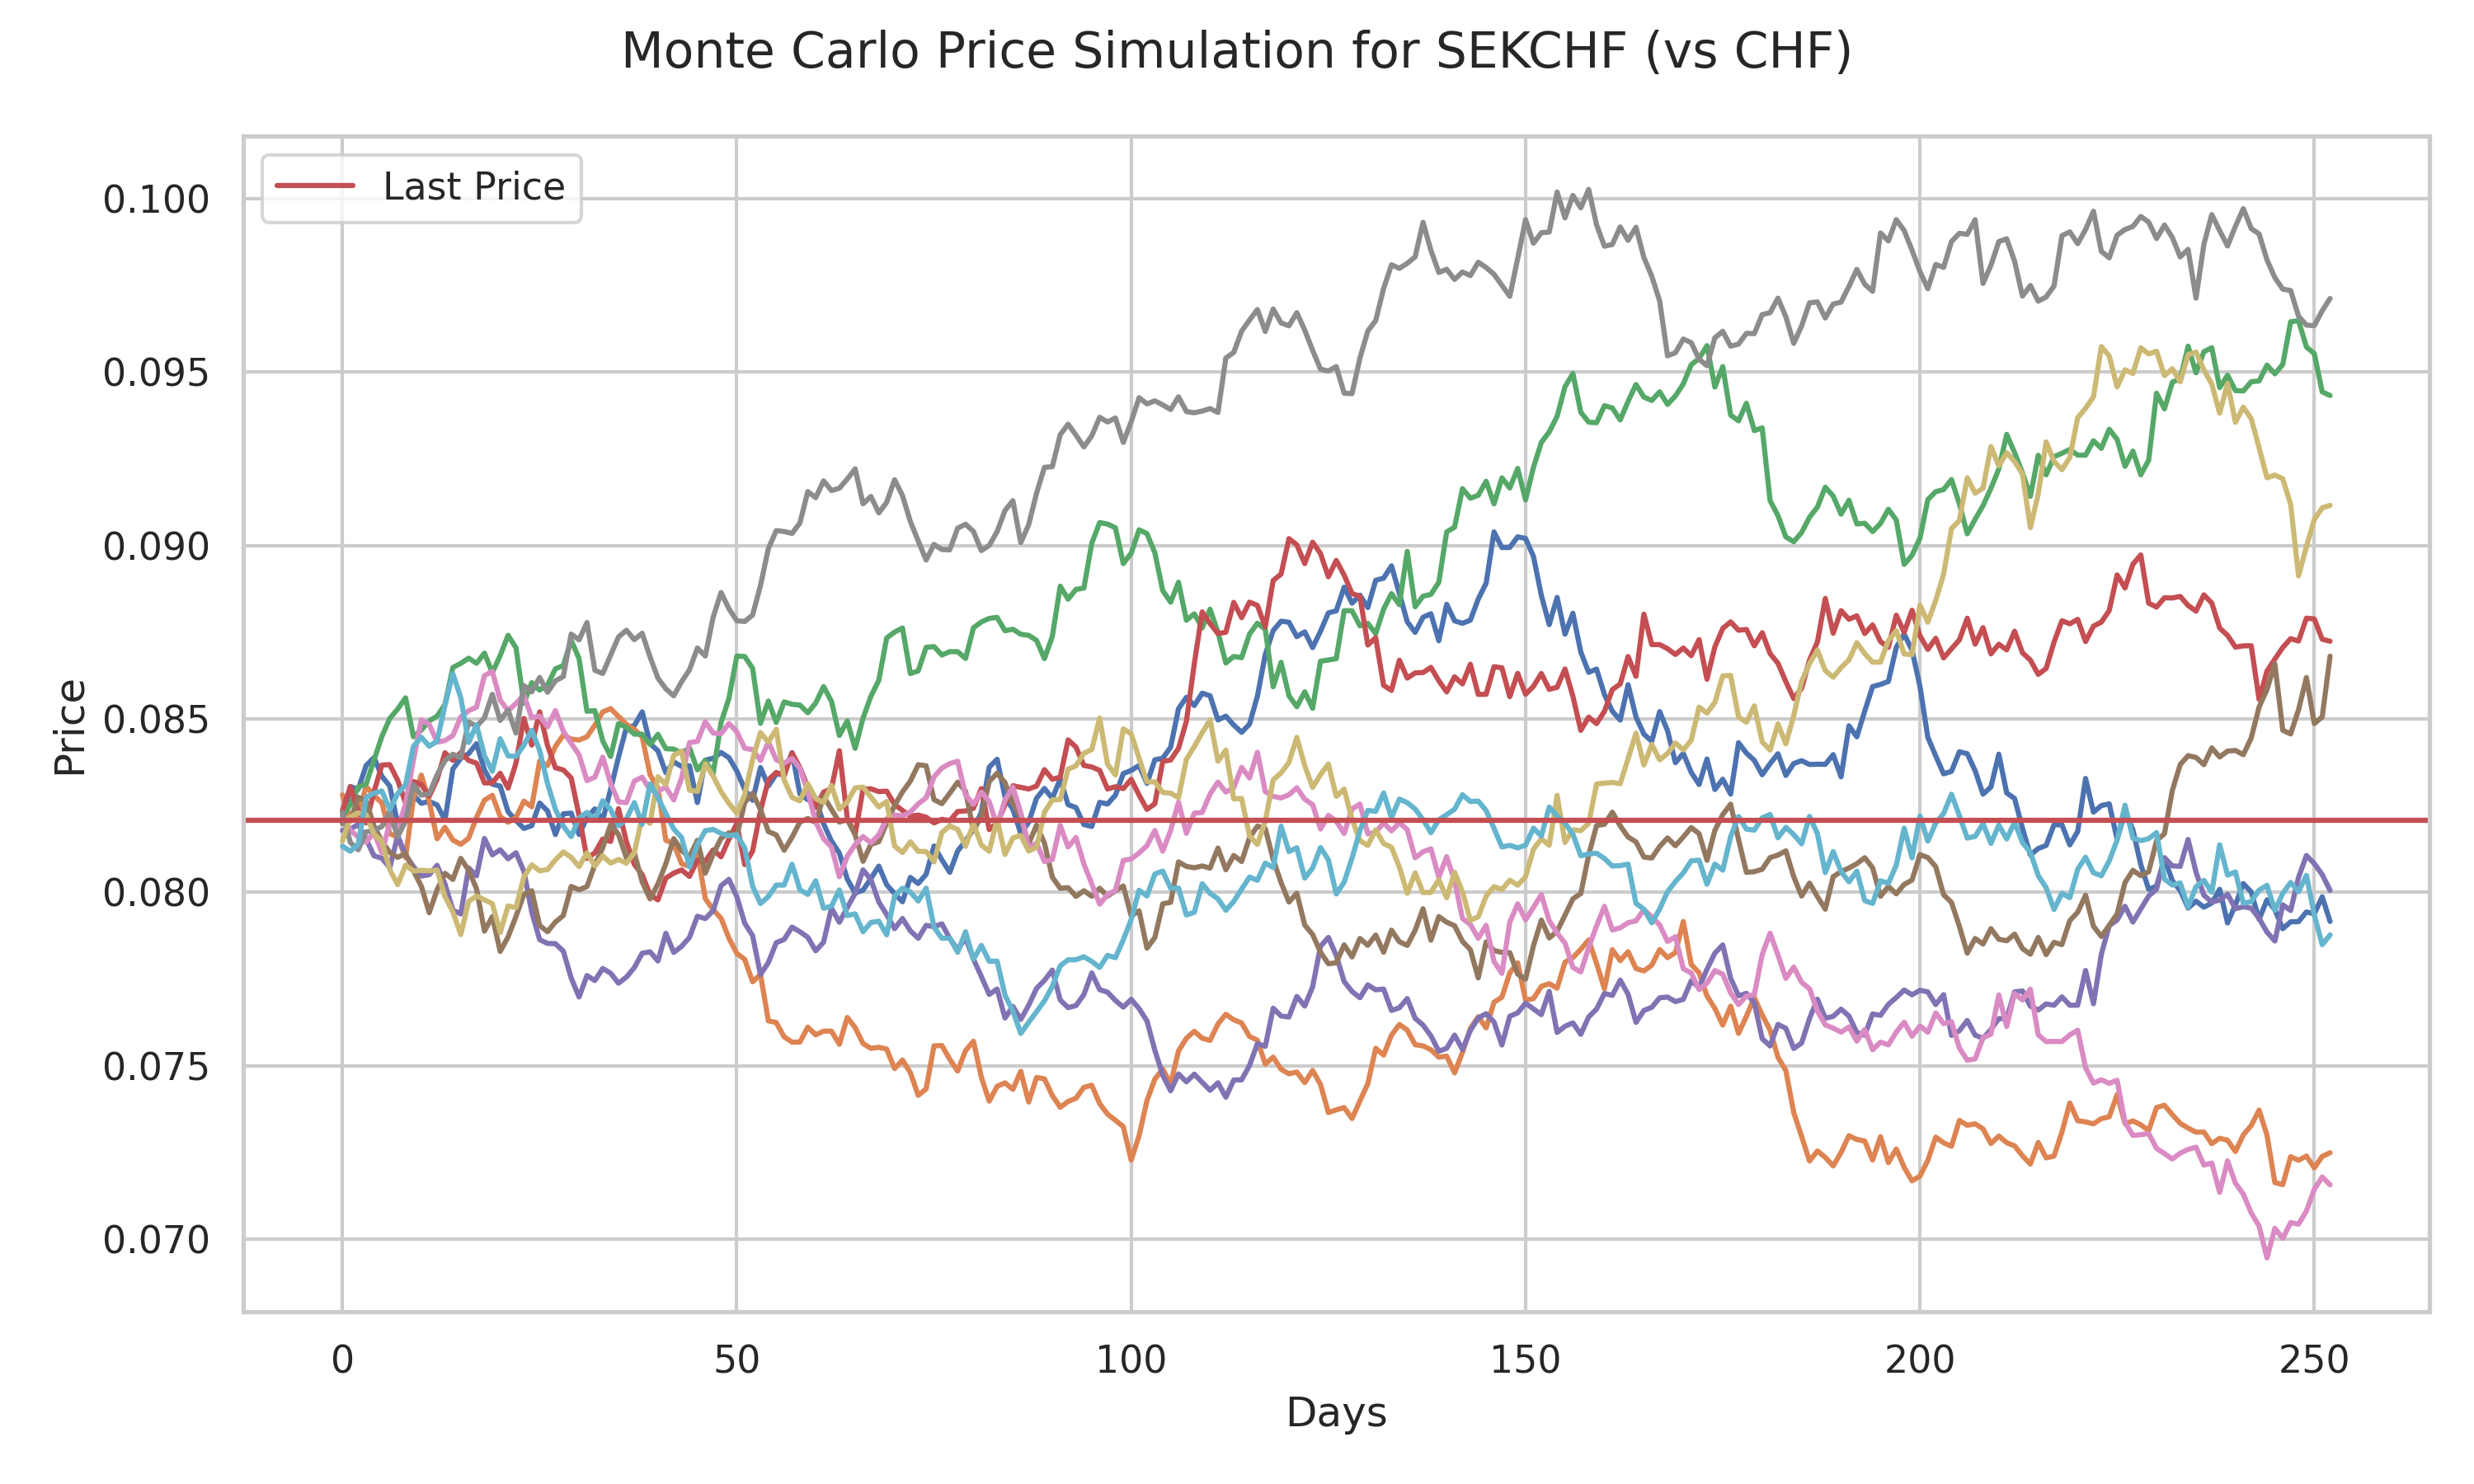
\includegraphics[width=0.48\linewidth]{reports/figures/monte_carlo_price_simulation_SEKCHF_vs_CHF.png} \label{fig:monte_carlo_price_simulation_SEKCHF_vs_CHF}
    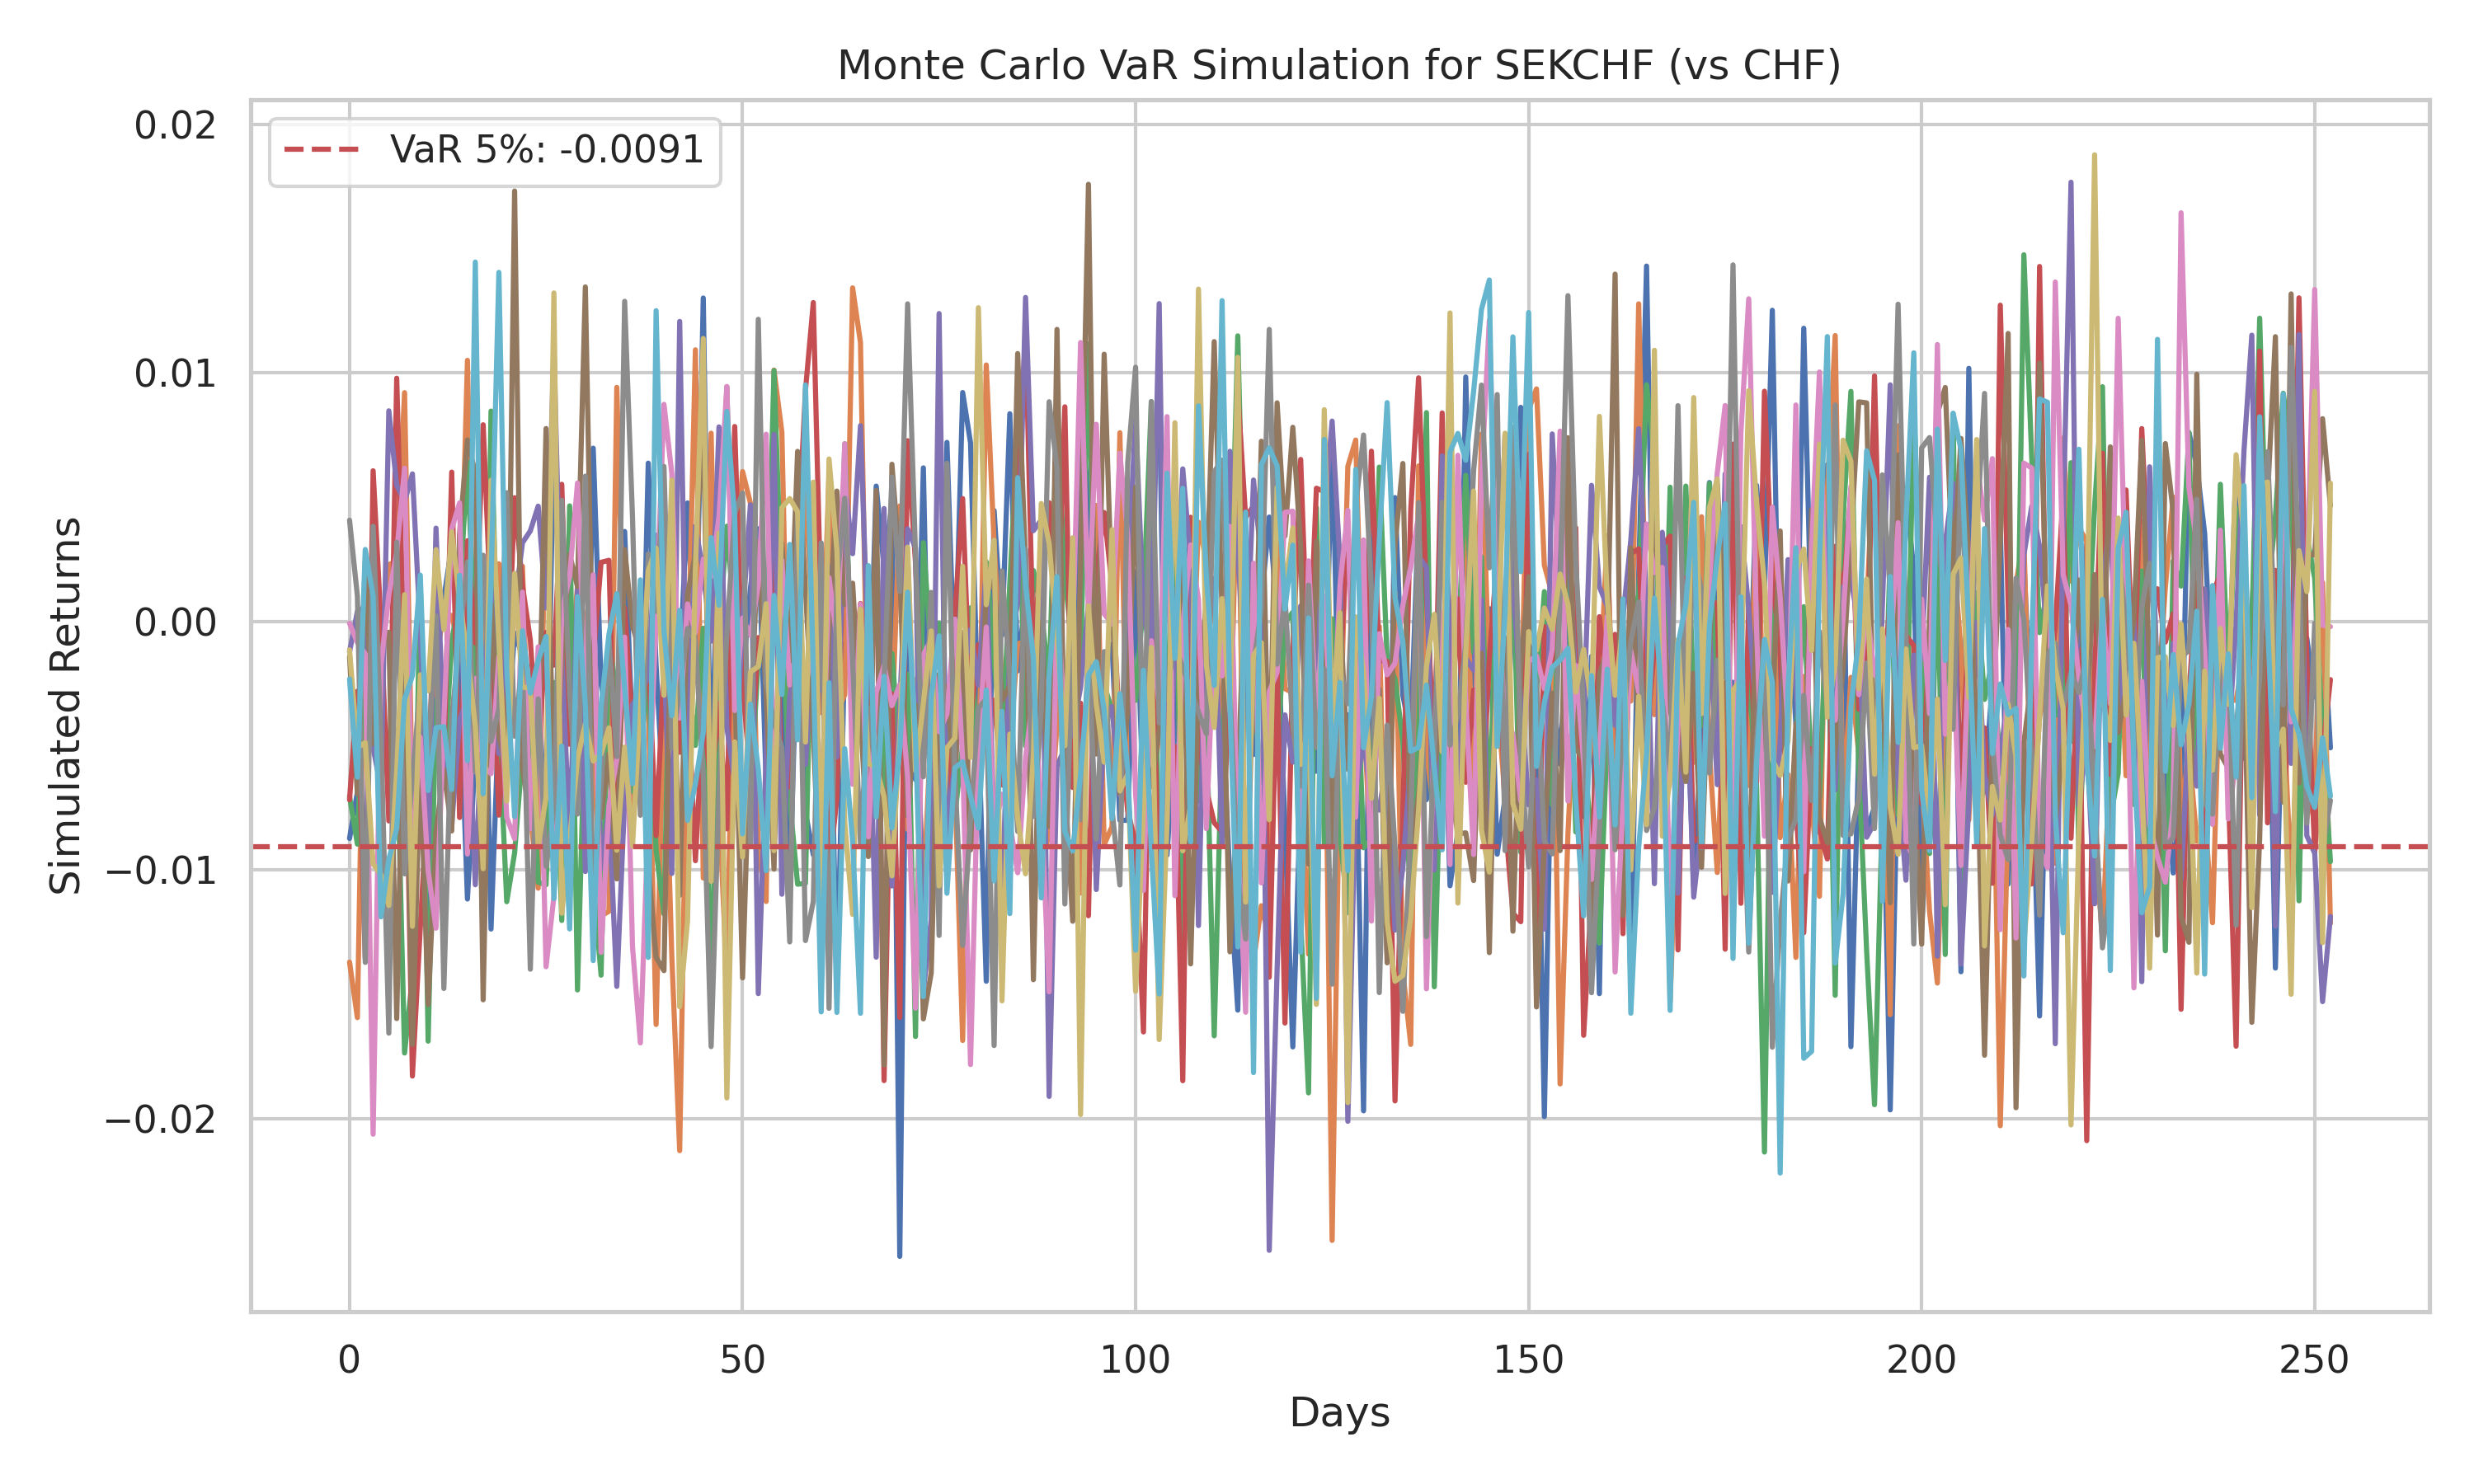
\includegraphics[width=0.48\linewidth]{reports/figures/monte_carlo_var_simulation_SEKCHF_vs_CHF.png} \label{fig:monte_carlo_var_simulation_SEKCHF_vs_CHF}
    \caption{\footnotesize Monte Carlo price siulation (left) and VaR simulation (right) for SEK-CHF.}
\end{figure}
\end{frame}
% ---------------------------------------------------------------------------
\begin{frame}
\frametitle{Main Findings}
\begin{figure}
    \centering  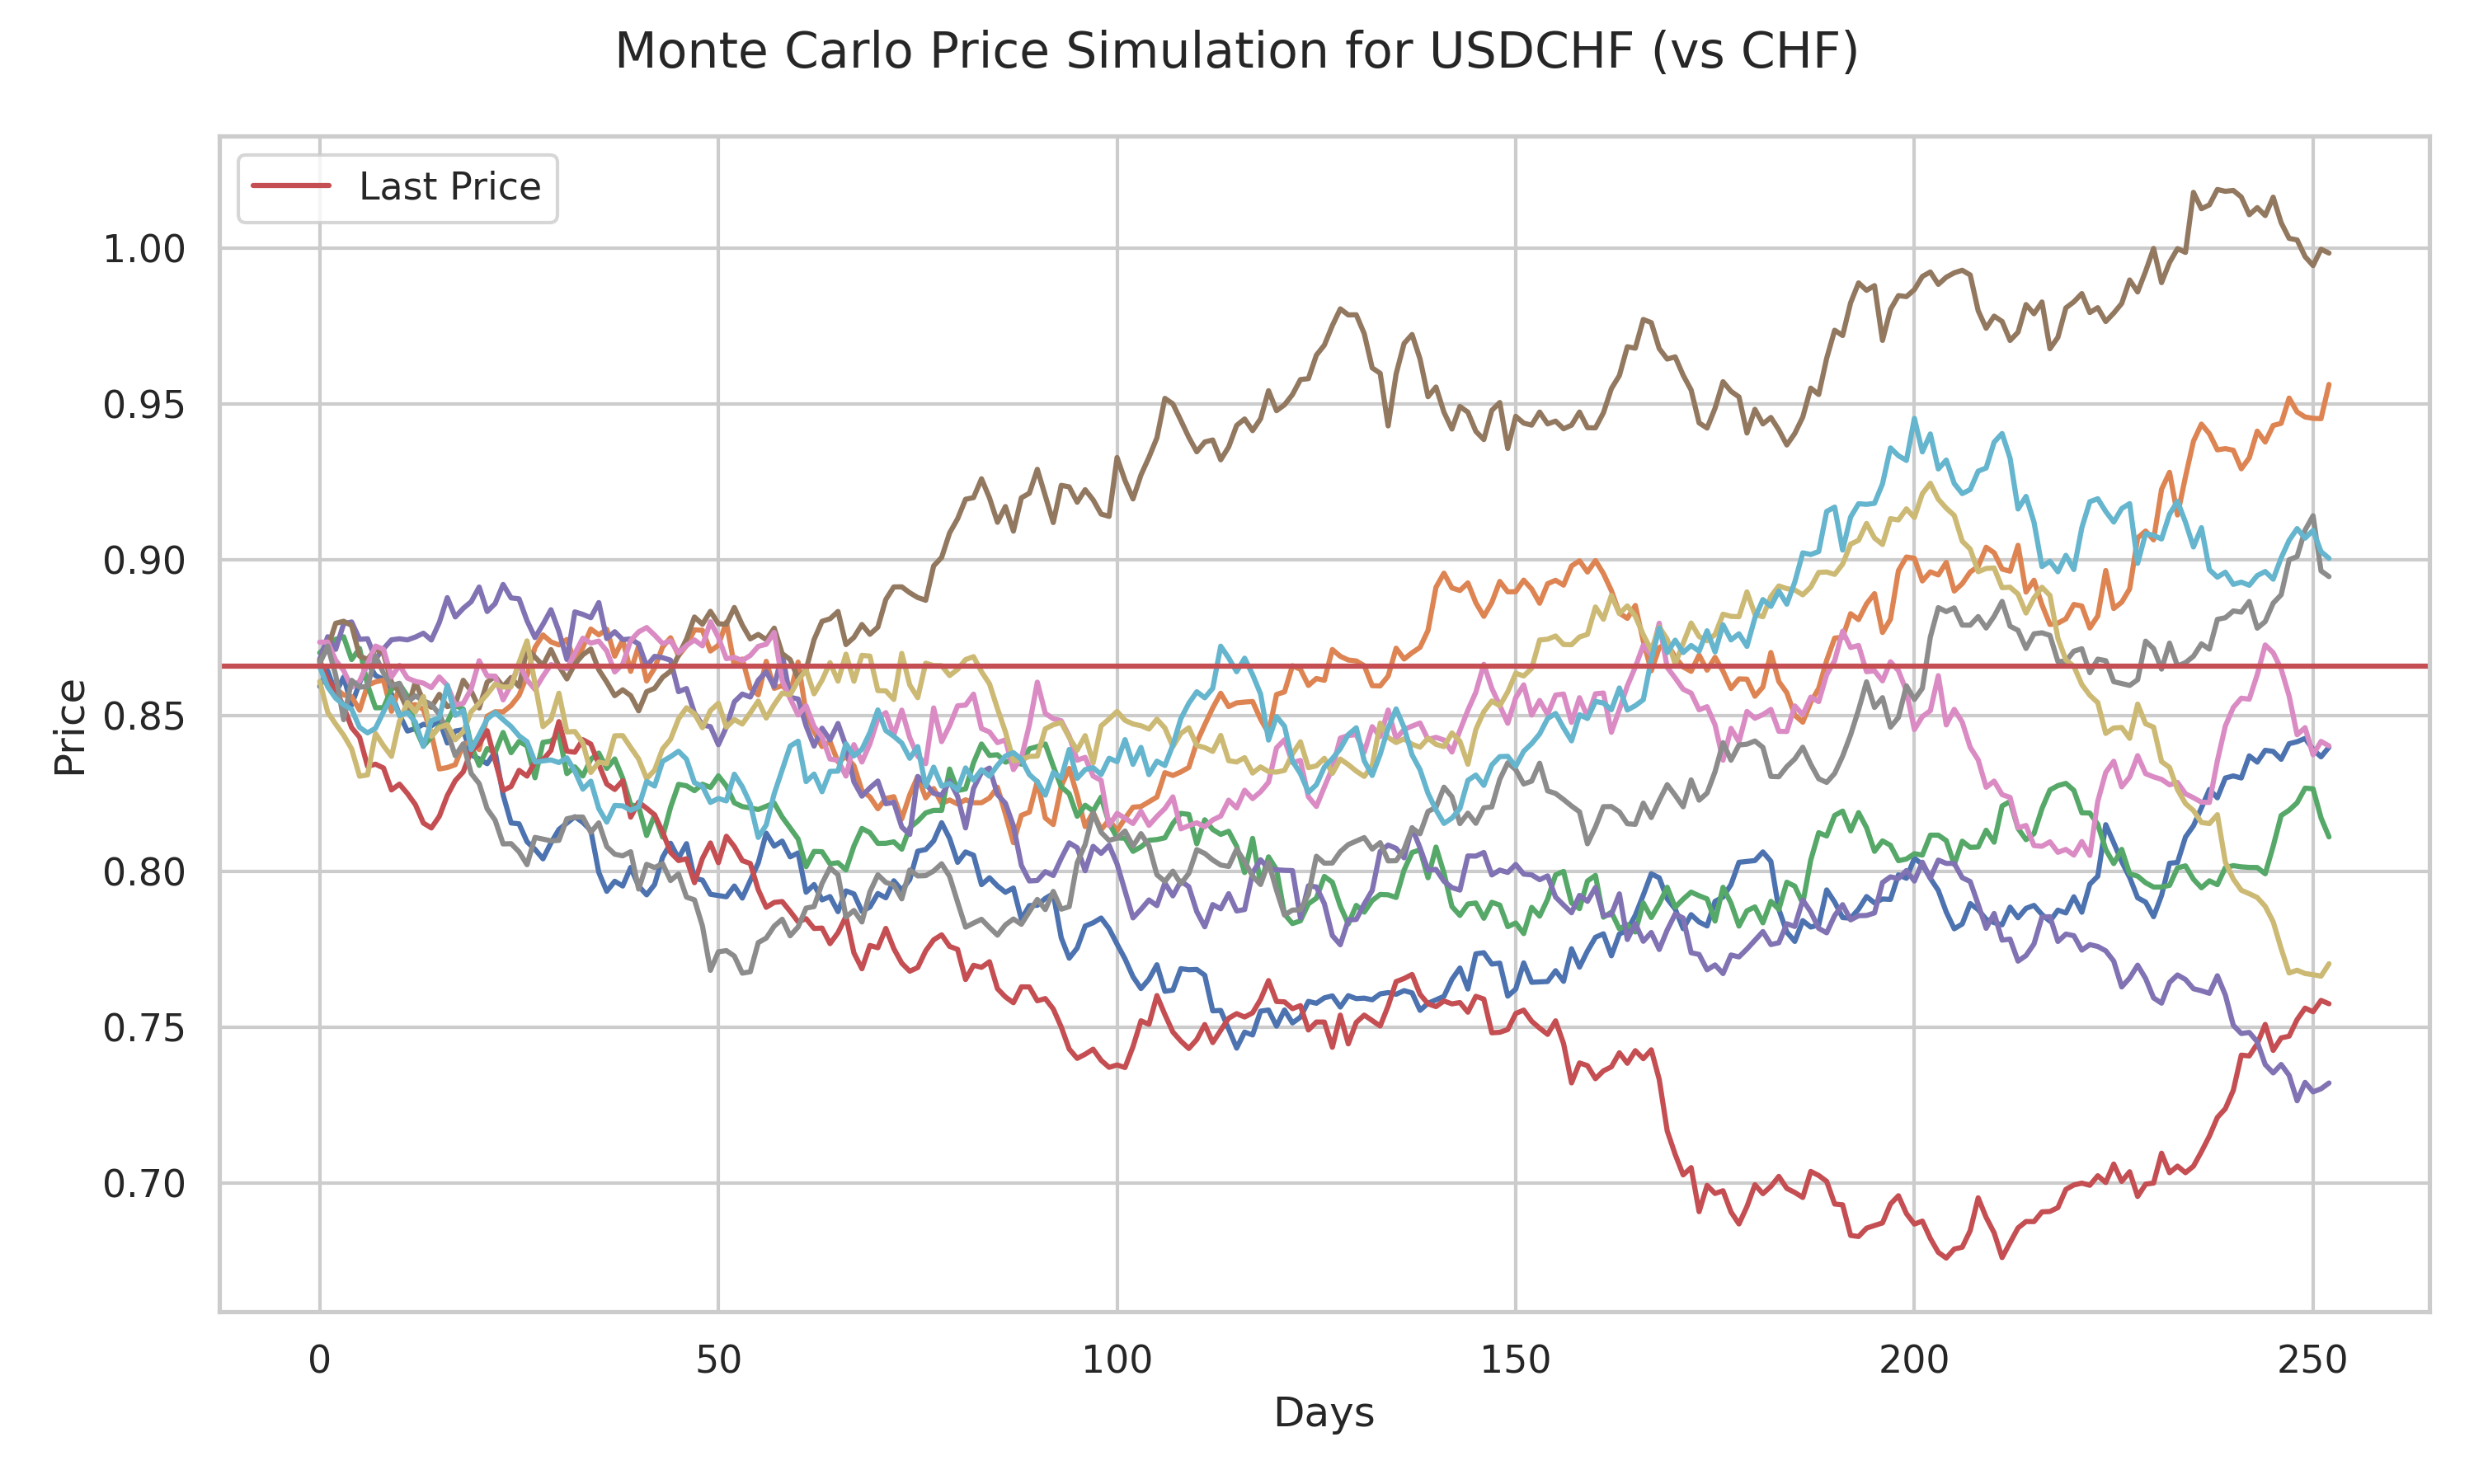
\includegraphics[width=0.48\linewidth]{reports/figures/monte_carlo_price_simulation_USDCHF_vs_CHF.png}  \label{fig:monte_carlo_price_simulation_USDCHF_vs_CHF}
    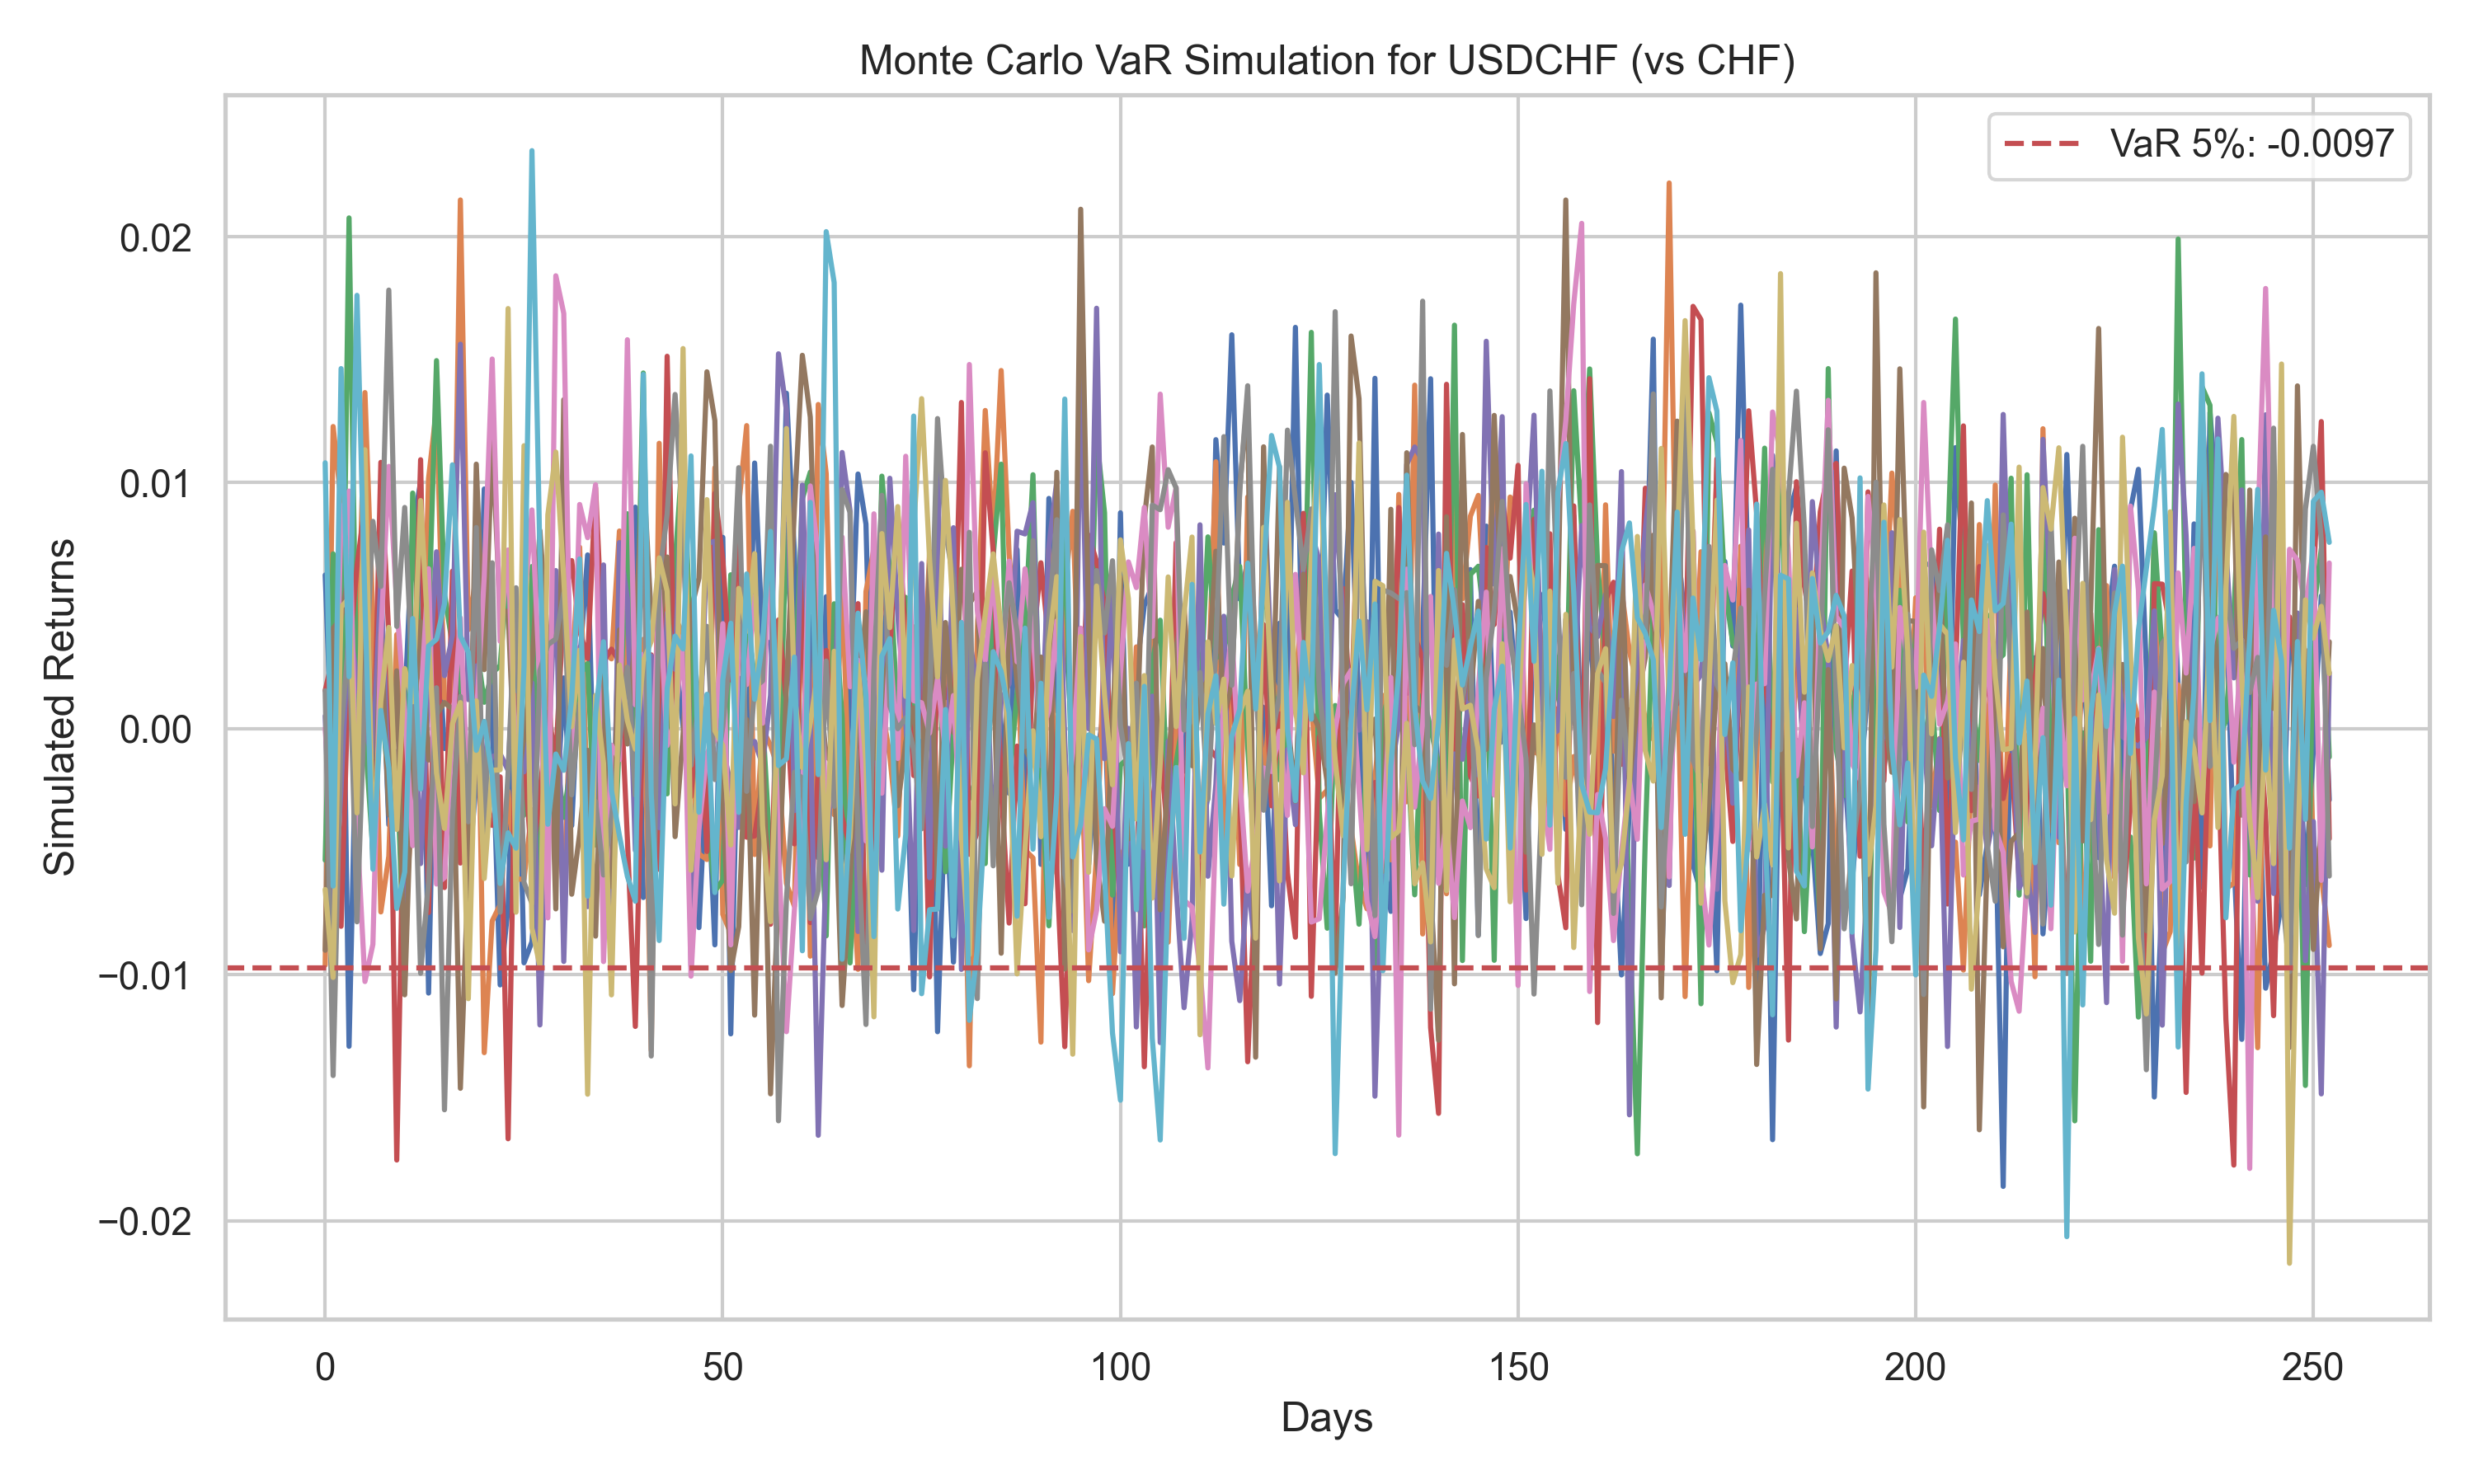
\includegraphics[width=0.49\linewidth]{reports/figures/monte_carlo_var_simulation_USDCHF_vs_CHF.png}  \label{fig:monte_carlo_var_simulation_USDCHF_vs_CHF}
    \caption{\footnotesize Monte Carlo price siulation (left) and VaR simulation (right) for USD-CHF.}
\end{figure}
\end{frame}
% ---------------------------------------------------------------------------
\begin{frame}
\section{Conclusion}
\frametitle{Conclusion}

\end{frame}
% ---------------------------------------------------------------------------

\end{document}
